% Options for packages loaded elsewhere
\PassOptionsToPackage{unicode}{hyperref}
\PassOptionsToPackage{hyphens}{url}
%
\documentclass[
]{scrreprt}
\usepackage{lmodern}
\usepackage{amssymb,amsmath}
\usepackage{ifxetex,ifluatex}
\ifnum 0\ifxetex 1\fi\ifluatex 1\fi=0 % if pdftex
  \usepackage[T1]{fontenc}
  \usepackage[utf8]{inputenc}
  \usepackage{textcomp} % provide euro and other symbols
\else % if luatex or xetex
  \usepackage{unicode-math}
  \defaultfontfeatures{Scale=MatchLowercase}
  \defaultfontfeatures[\rmfamily]{Ligatures=TeX,Scale=1}
\fi
% Use upquote if available, for straight quotes in verbatim environments
\IfFileExists{upquote.sty}{\usepackage{upquote}}{}
\IfFileExists{microtype.sty}{% use microtype if available
  \usepackage[]{microtype}
  \UseMicrotypeSet[protrusion]{basicmath} % disable protrusion for tt fonts
}{}
\makeatletter
\@ifundefined{KOMAClassName}{% if non-KOMA class
  \IfFileExists{parskip.sty}{%
    \usepackage{parskip}
  }{% else
    \setlength{\parindent}{0pt}
    \setlength{\parskip}{6pt plus 2pt minus 1pt}}
}{% if KOMA class
  \KOMAoptions{parskip=half}}
\makeatother
\usepackage{xcolor}
\IfFileExists{xurl.sty}{\usepackage{xurl}}{} % add URL line breaks if available
\IfFileExists{bookmark.sty}{\usepackage{bookmark}}{\usepackage{hyperref}}
\hypersetup{
  pdftitle={A Rough Guide to Pre-processing High-Frequency Animal Tracking Data},
  pdfauthor={Pratik R. Gupte and others},
  hidelinks,
  pdfcreator={LaTeX via pandoc}}
\urlstyle{same} % disable monospaced font for URLs
\usepackage[left=4cm, right=3cm, top=2.5cm, bottom=2.5cm]{geometry}
\usepackage{color}
\usepackage{fancyvrb}
\newcommand{\VerbBar}{|}
\newcommand{\VERB}{\Verb[commandchars=\\\{\}]}
\DefineVerbatimEnvironment{Highlighting}{Verbatim}{commandchars=\\\{\}}
% Add ',fontsize=\small' for more characters per line
\newenvironment{Shaded}{}{}
\newcommand{\AlertTok}[1]{\textcolor[rgb]{1.00,0.00,0.00}{\textbf{#1}}}
\newcommand{\AnnotationTok}[1]{\textcolor[rgb]{0.38,0.63,0.69}{\textbf{\textit{#1}}}}
\newcommand{\AttributeTok}[1]{\textcolor[rgb]{0.49,0.56,0.16}{#1}}
\newcommand{\BaseNTok}[1]{\textcolor[rgb]{0.25,0.63,0.44}{#1}}
\newcommand{\BuiltInTok}[1]{#1}
\newcommand{\CharTok}[1]{\textcolor[rgb]{0.25,0.44,0.63}{#1}}
\newcommand{\CommentTok}[1]{\textcolor[rgb]{0.38,0.63,0.69}{\textit{#1}}}
\newcommand{\CommentVarTok}[1]{\textcolor[rgb]{0.38,0.63,0.69}{\textbf{\textit{#1}}}}
\newcommand{\ConstantTok}[1]{\textcolor[rgb]{0.53,0.00,0.00}{#1}}
\newcommand{\ControlFlowTok}[1]{\textcolor[rgb]{0.00,0.44,0.13}{\textbf{#1}}}
\newcommand{\DataTypeTok}[1]{\textcolor[rgb]{0.56,0.13,0.00}{#1}}
\newcommand{\DecValTok}[1]{\textcolor[rgb]{0.25,0.63,0.44}{#1}}
\newcommand{\DocumentationTok}[1]{\textcolor[rgb]{0.73,0.13,0.13}{\textit{#1}}}
\newcommand{\ErrorTok}[1]{\textcolor[rgb]{1.00,0.00,0.00}{\textbf{#1}}}
\newcommand{\ExtensionTok}[1]{#1}
\newcommand{\FloatTok}[1]{\textcolor[rgb]{0.25,0.63,0.44}{#1}}
\newcommand{\FunctionTok}[1]{\textcolor[rgb]{0.02,0.16,0.49}{#1}}
\newcommand{\ImportTok}[1]{#1}
\newcommand{\InformationTok}[1]{\textcolor[rgb]{0.38,0.63,0.69}{\textbf{\textit{#1}}}}
\newcommand{\KeywordTok}[1]{\textcolor[rgb]{0.00,0.44,0.13}{\textbf{#1}}}
\newcommand{\NormalTok}[1]{#1}
\newcommand{\OperatorTok}[1]{\textcolor[rgb]{0.40,0.40,0.40}{#1}}
\newcommand{\OtherTok}[1]{\textcolor[rgb]{0.00,0.44,0.13}{#1}}
\newcommand{\PreprocessorTok}[1]{\textcolor[rgb]{0.74,0.48,0.00}{#1}}
\newcommand{\RegionMarkerTok}[1]{#1}
\newcommand{\SpecialCharTok}[1]{\textcolor[rgb]{0.25,0.44,0.63}{#1}}
\newcommand{\SpecialStringTok}[1]{\textcolor[rgb]{0.73,0.40,0.53}{#1}}
\newcommand{\StringTok}[1]{\textcolor[rgb]{0.25,0.44,0.63}{#1}}
\newcommand{\VariableTok}[1]{\textcolor[rgb]{0.10,0.09,0.49}{#1}}
\newcommand{\VerbatimStringTok}[1]{\textcolor[rgb]{0.25,0.44,0.63}{#1}}
\newcommand{\WarningTok}[1]{\textcolor[rgb]{0.38,0.63,0.69}{\textbf{\textit{#1}}}}
\usepackage{longtable,booktabs}
% Correct order of tables after \paragraph or \subparagraph
\usepackage{etoolbox}
\makeatletter
\patchcmd\longtable{\par}{\if@noskipsec\mbox{}\fi\par}{}{}
\makeatother
% Allow footnotes in longtable head/foot
\IfFileExists{footnotehyper.sty}{\usepackage{footnotehyper}}{\usepackage{footnote}}
\makesavenoteenv{longtable}
\usepackage{graphicx}
\makeatletter
\def\maxwidth{\ifdim\Gin@nat@width>\linewidth\linewidth\else\Gin@nat@width\fi}
\def\maxheight{\ifdim\Gin@nat@height>\textheight\textheight\else\Gin@nat@height\fi}
\makeatother
% Scale images if necessary, so that they will not overflow the page
% margins by default, and it is still possible to overwrite the defaults
% using explicit options in \includegraphics[width, height, ...]{}
\setkeys{Gin}{width=\maxwidth,height=\maxheight,keepaspectratio}
% Set default figure placement to htbp
\makeatletter
\def\fps@figure{htbp}
\makeatother
\setlength{\emergencystretch}{3em} % prevent overfull lines
\providecommand{\tightlist}{%
  \setlength{\itemsep}{0pt}\setlength{\parskip}{0pt}}
\setcounter{secnumdepth}{2}

\usepackage{fontspec}
% use nice fonts if available else use boring defaults
\IfFontExistsTF{IBM Plex Mono}{\setmonofont[]{IBM Plex Mono}}{}

\usepackage{lineno}
\usepackage{tgtermes}
\newlength{\cslhangindent}
\setlength{\cslhangindent}{1.5em}
\newenvironment{cslreferences}%
  {\setlength{\parindent}{0pt}%
  \everypar{\setlength{\hangindent}{\cslhangindent}}\ignorespaces}%
  {\par}

\title{A Rough Guide to Pre-processing High-Frequency Animal Tracking Data}
\author{Pratik R. Gupte and others}
\date{2020-10-29}

\begin{document}
\maketitle

{
\setcounter{tocdepth}{1}
\tableofcontents
}
\hypertarget{abstract}{%
\chapter{Abstract}\label{abstract}}

Data cleaning is a ubiquitous pre-processing step in analysis pipelines, and its automation is essential for large data volumes such as those generated in animal tracking studies using high-frequency Time-of-Arrival (TOA) systems.
Users of systems such as ATLAS must contend with two intertwined data cleaning challenges: (1) reducing positioning errors, and (2) the high volume of data itself.
Making biological inferences from data with positioning errors is not straightforward, and processing large data volumes is computationally intensive.
Though reducing positioning error is widely recommended, users are without uniform guidance on how to go about this, and lack a common set of computationally efficient tools.
Further, many methods that synthesize movement tracks for ecological inference are either (1) not suited to very large datasets, or (2) not intuitive to understand in terms of the tracked animal's biology.

In this article we introduce a pipeline to pre-process high-frequency animal tracking data in order to prepare it for subsequent analysis.
We demonstrate this pipeline on simulated movement data to which we have randomly added positioning errors.
This pipeline is suited to any tracking study in which the high data volume combined with knowledge of the tracked individuals' biology can be used to smooth out positioning errors.
We further suggest how large volumes of cleaned data may be synthesized into biologically meaningful `residence patches', and demonstrate how this accurately captures animal space-use.
Finally, we introduce the \texttt{R} package \texttt{atlastools} which provides fast implementations of the methods we describe.
Though aimed at ATLAS systems, \texttt{atlastools} can be used with any time-series animal movement data, and we demonstrate its usage with both simulated and empirical examples.

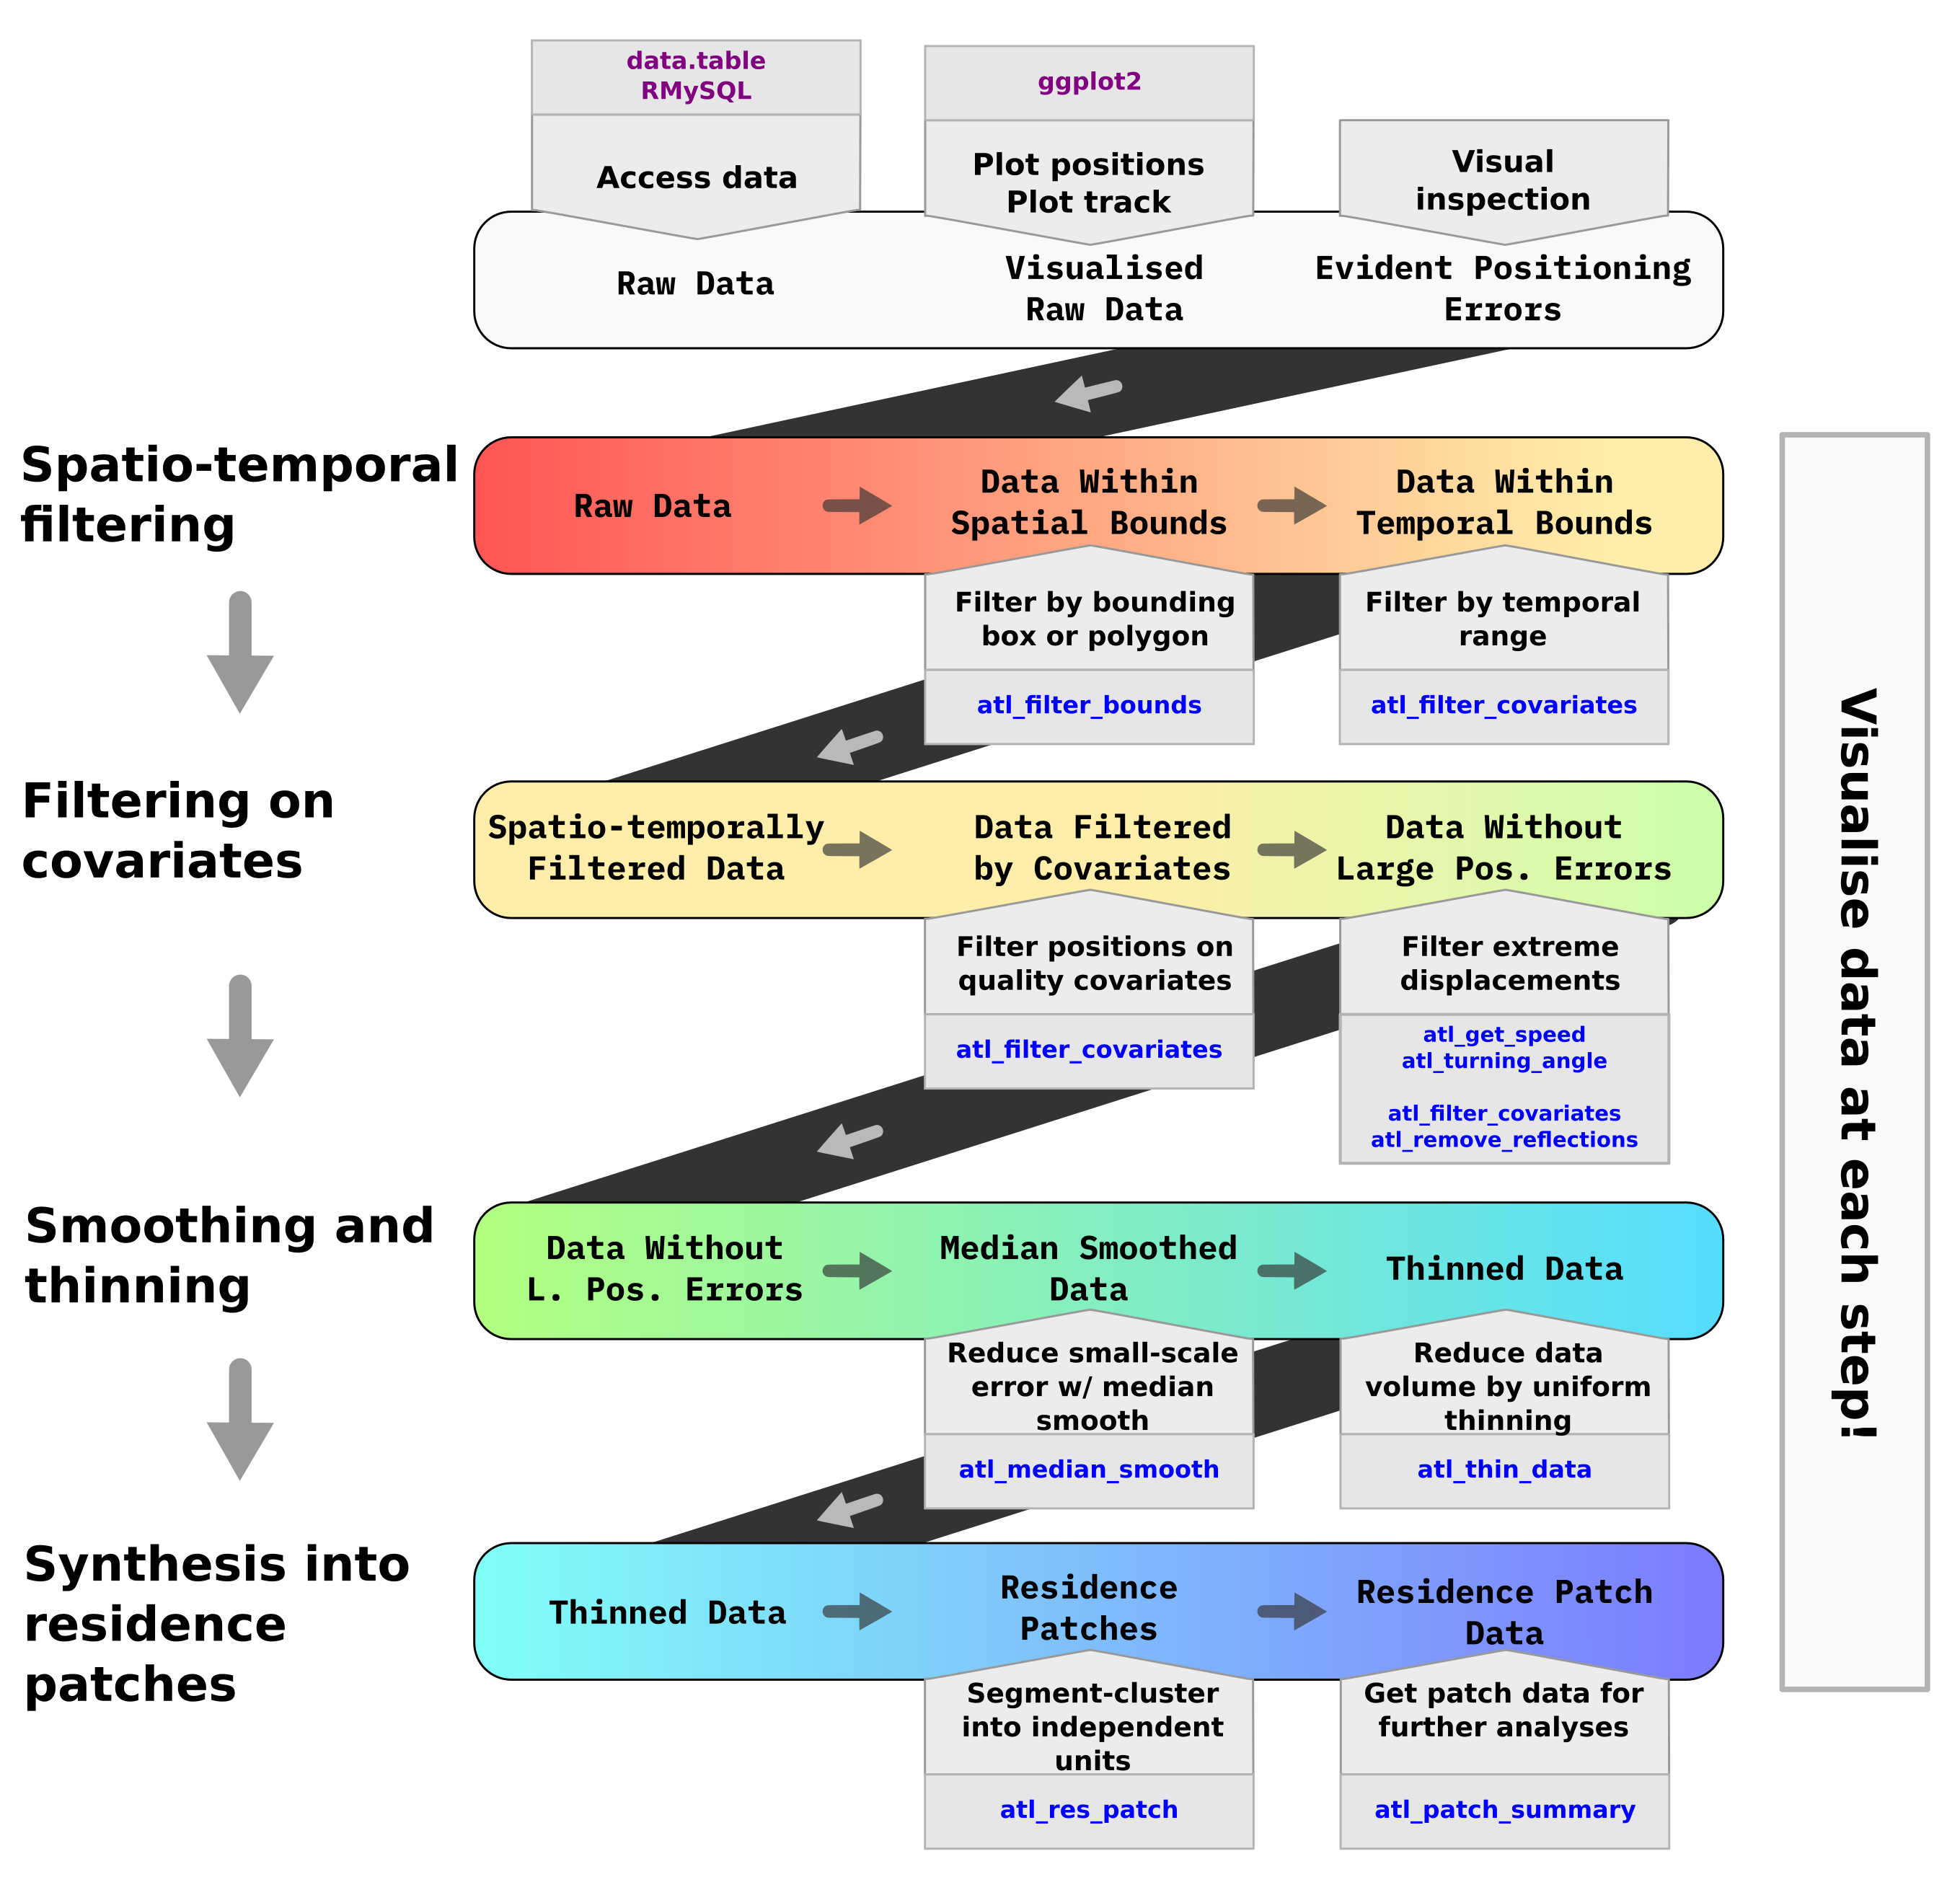
\includegraphics{figures/fig_recipe.png}

\hypertarget{getting-started}{%
\chapter{Getting started}\label{getting-started}}

This section covers:

\begin{enumerate}
\def\labelenumi{\arabic{enumi}.}
\item
  Installing the \texttt{R} package \texttt{atlastools},
\item
  Simulating some realistic looking movement data using the \texttt{R} package \texttt{smoove} from (Gurarie et al. \protect\hyperlink{ref-gurarie2017}{2017}), and
\item
  Introducing positioning errors into the simulated movement data.
\end{enumerate}

\hypertarget{installing-atlastools}{%
\section{\texorpdfstring{Installing \texttt{atlastools}}{Installing atlastools}}\label{installing-atlastools}}

This paper refers extensively to the \texttt{R} package \texttt{atlastools} (Gupte 2020), which can be installed from \href{https://github.com/pratikunterwegs/atlastools}{Github}.

Releases of the package from Github can be found on Zenodo: (\url{https://doi.org/10.5281/zenodo.4033155})

The code chunk below shows how to install \texttt{atlastools}.

\begin{Shaded}
\begin{Highlighting}[]
\CommentTok{\# use either devtools or remotes to install}
\KeywordTok{install.packages}\NormalTok{(}\StringTok{"devtools"}\NormalTok{)}

\CommentTok{\# installation using devtools}
\NormalTok{devtools}\OperatorTok{::}\KeywordTok{install\_github}\NormalTok{(}\StringTok{"pratikunterwegs/atlastools"}\NormalTok{)}
\end{Highlighting}
\end{Shaded}

\hypertarget{simulating-movement-data}{%
\section{Simulating movement data}\label{simulating-movement-data}}

Here, we simulate some movement data using the \texttt{smoove} \texttt{R} package from (Gurarie et al. \protect\hyperlink{ref-gurarie2017}{2017}).

First, we load \texttt{smoove} and \texttt{data.table}, as well as some helper functions that make use of them to simulate data for use.

\begin{Shaded}
\begin{Highlighting}[]
\CommentTok{\# load smoove and datatable}
\KeywordTok{library}\NormalTok{(smoove)}
\KeywordTok{library}\NormalTok{(data.table)}

\CommentTok{\# source helper functions}
\KeywordTok{source}\NormalTok{(}\StringTok{"R/helper\_functions.R"}\NormalTok{)}
\end{Highlighting}
\end{Shaded}

\begin{Shaded}
\begin{Highlighting}[]
\NormalTok{data <{-}}\StringTok{ }\KeywordTok{do\_smoove\_data}\NormalTok{()}
\CommentTok{\# save simulated data}
\KeywordTok{fwrite}\NormalTok{(data, }\StringTok{"data/data\_sim.csv"}\NormalTok{)}
\end{Highlighting}
\end{Shaded}

\hypertarget{simualte-for-residence-patches}{%
\section{Simualte for residence patches}\label{simualte-for-residence-patches}}

\begin{Shaded}
\begin{Highlighting}[]
\CommentTok{\# do smoove data using a RACVM}
\NormalTok{data <{-}}\StringTok{ }\NormalTok{smoove}\OperatorTok{::}\KeywordTok{simulateRACVM}\NormalTok{(}\DataTypeTok{dt =} \FloatTok{0.1}\NormalTok{, }\DataTypeTok{Tmax =} \DecValTok{500}\NormalTok{, }\DataTypeTok{omega =} \DecValTok{5}\NormalTok{, }\DataTypeTok{v0 =} \DecValTok{1}\NormalTok{, }\DataTypeTok{mu =} \FloatTok{0.1}\NormalTok{)}
\NormalTok{data <{-}}\StringTok{ }\KeywordTok{as.data.table}\NormalTok{(data}\OperatorTok{$}\NormalTok{XY)}

\CommentTok{\# assign id}
\NormalTok{data[, id }\OperatorTok{:}\ErrorTok{=}\StringTok{ "test"}\NormalTok{]}
\NormalTok{data[, time }\OperatorTok{:}\ErrorTok{=}\StringTok{ }\KeywordTok{seq\_len}\NormalTok{(}\KeywordTok{nrow}\NormalTok{(data))]}
\CommentTok{\# rename x and y}
\KeywordTok{setnames}\NormalTok{(data, }\DataTypeTok{old =} \KeywordTok{c}\NormalTok{(}\StringTok{"x"}\NormalTok{, }\StringTok{"y"}\NormalTok{), }\DataTypeTok{new =} \KeywordTok{c}\NormalTok{(}\StringTok{"y"}\NormalTok{, }\StringTok{"x"}\NormalTok{))}

\CommentTok{\# save data}
\KeywordTok{fwrite}\NormalTok{(data, }\StringTok{"data/data\_for\_res\_patch.csv"}\NormalTok{)}
\end{Highlighting}
\end{Shaded}

\hypertarget{reducing-large-scale-positioning-error-by-filtering-data}{%
\chapter{Reducing Large-Scale Positioning Error by Filtering Data}\label{reducing-large-scale-positioning-error-by-filtering-data}}

\hypertarget{prepare-libraries}{%
\section{Prepare Libraries}\label{prepare-libraries}}

Here we load some useful libraries, and the helper functions.

\begin{Shaded}
\begin{Highlighting}[]
\CommentTok{\# to handle movement data}
\KeywordTok{library}\NormalTok{(data.table)}
\KeywordTok{library}\NormalTok{(atlastools)}

\CommentTok{\# to plot}
\KeywordTok{library}\NormalTok{(ggplot2)}
\KeywordTok{library}\NormalTok{(patchwork)}
\end{Highlighting}
\end{Shaded}

\begin{Shaded}
\begin{Highlighting}[]
\CommentTok{\# source helper functions}
\KeywordTok{source}\NormalTok{(}\StringTok{"R/helper\_functions.R"}\NormalTok{)}
\end{Highlighting}
\end{Shaded}

\hypertarget{introducing-errors-to-the-data}{%
\section{Introducing Errors to the Data}\label{introducing-errors-to-the-data}}

Here we introduce three kinds of errors to the data:

\begin{enumerate}
\def\labelenumi{\arabic{enumi}.}
\item
  Small-scale normally distributed errors at each position;
\item
  Large-scale error at a random 0.5\% of positions;
\item
  A large-scale displacement of a sequence of 300 positions.
\end{enumerate}

While the data are 10,000 positions at 1-second interval, we shall use only 5,000 of these.

\begin{Shaded}
\begin{Highlighting}[]
\CommentTok{\# read in the data}
\NormalTok{data <{-}}\StringTok{ }\KeywordTok{fread}\NormalTok{(}\StringTok{"data/data\_sim.csv"}\NormalTok{)[}\DecValTok{5000}\OperatorTok{:}\DecValTok{10000}\NormalTok{, ]}
\end{Highlighting}
\end{Shaded}

We add outliers at random to the data to demonstrate their removal.

\begin{Shaded}
\begin{Highlighting}[]
\CommentTok{\# make a copy}
\NormalTok{data\_copy <{-}}\StringTok{ }\KeywordTok{copy}\NormalTok{(data)}

\CommentTok{\# add a prolonged spike or reflection to 300 positions}
\NormalTok{data\_copy[}\DecValTok{500}\OperatorTok{:}\DecValTok{800}\NormalTok{, }\StringTok{\textasciigrave{}}\DataTypeTok{:=}\StringTok{\textasciigrave{}}\NormalTok{(}\DataTypeTok{x =}\NormalTok{ x }\OperatorTok{+}\StringTok{ }\FloatTok{0.25}\NormalTok{,}
                        \DataTypeTok{y =}\NormalTok{ y }\OperatorTok{+}\StringTok{ }\FloatTok{0.25}\NormalTok{)]}

\CommentTok{\# add normal error}
\NormalTok{data\_copy[, }\StringTok{\textasciigrave{}}\DataTypeTok{:=}\StringTok{\textasciigrave{}}\NormalTok{(}\DataTypeTok{x =} \KeywordTok{do\_add\_error}\NormalTok{(x, }\DataTypeTok{std\_dev =} \FloatTok{0.01}\NormalTok{),}
                 \DataTypeTok{y =} \KeywordTok{do\_add\_error}\NormalTok{(y, }\DataTypeTok{std\_dev =} \FloatTok{0.005}\NormalTok{))]}

\CommentTok{\# add 100 outliers}
\NormalTok{data\_copy <{-}}\StringTok{ }\KeywordTok{do\_add\_outliers}\NormalTok{(data\_copy, }\DataTypeTok{p\_data =} \FloatTok{0.005}\NormalTok{, }\DataTypeTok{std\_dev =} \FloatTok{0.1}\NormalTok{)}
\end{Highlighting}
\end{Shaded}

Save the data to which errors have been added.

\begin{Shaded}
\begin{Highlighting}[]
\KeywordTok{fwrite}\NormalTok{(data\_copy, }\DataTypeTok{file =} \StringTok{"data/data\_errors.csv"}\NormalTok{)}
\end{Highlighting}
\end{Shaded}

\begin{Shaded}
\begin{Highlighting}[]
\NormalTok{data\_copy <{-}}\StringTok{ }\KeywordTok{fread}\NormalTok{(}\StringTok{"data/data\_errors.csv"}\NormalTok{)}
\end{Highlighting}
\end{Shaded}

Define a palette with 4 colours for convenience.

\begin{Shaded}
\begin{Highlighting}[]
\CommentTok{\# define a four colour palette}
\NormalTok{pal <{-}}\StringTok{ }\NormalTok{RColorBrewer}\OperatorTok{::}\KeywordTok{brewer.pal}\NormalTok{(}\DecValTok{4}\NormalTok{, }\StringTok{"Set1"}\NormalTok{)}
\end{Highlighting}
\end{Shaded}

We make a figure of the canonical data (grey line) along with the artificially added error (grey points).

\hypertarget{filtering-by-spatial-bounds}{%
\section{Filtering by Spatial Bounds}\label{filtering-by-spatial-bounds}}

Filtering by spatial bounds is a good way to begin reducing gross, large-scale positioning errors.
There are two main ways of doing this:

\begin{enumerate}
\def\labelenumi{\arabic{enumi}.}
\item
  Filtering by a bounding box: Compare the coordinates of observations against a range of acceptable coordinates, and retain those which fall within the range, or
\item
  Filtering by a spatial polygon: An explicit geometric intersection between the positions and a polygon representing an area of interest.
\end{enumerate}

Here, we remove gross positioning errors using a bounding box filter using the function \texttt{atl\_filter\_bounds}. In this example, we show filtering only on the Y coordinate.

\texttt{atl\_filter\_bounds} takes coordinate ranges as two-element vectors of the lower and higher bound.
It is possible to pass one of the bounds as \texttt{NA}, in which case, only the other bound is used for filtering, i.e., \texttt{y\_range\ =\ c(NA,\ 1)} is equivalent to selecting all Y coordinates \textless{} 1.

\texttt{atl\_filter\_bounds} was initially designed to remove positions \emph{inside} a specific range, hence the argument \texttt{remove\_inside}.
The default value of the argument is \texttt{FALSE}, and \texttt{atl\_filter\_bounds} is thus a bounding box filter.

\begin{Shaded}
\begin{Highlighting}[]
\CommentTok{\# remove positions outside a bounding box}
\CommentTok{\# NB: set remove\_inside to FALSE}
\NormalTok{data\_inside\_bbox <{-}}\StringTok{ }\KeywordTok{atl\_filter\_bounds}\NormalTok{(}\DataTypeTok{data =}\NormalTok{ data\_copy,}
                                      \DataTypeTok{y\_range =} \KeywordTok{c}\NormalTok{(}\FloatTok{0.5}\NormalTok{, }\DecValTok{1}\NormalTok{),}
                                      \DataTypeTok{remove\_inside =} \OtherTok{FALSE}\NormalTok{)}
\end{Highlighting}
\end{Shaded}

\texttt{atl\_filter\_bounds} is not vectorised, and if there are two or more bounds per coordinate (for instance, \(X_1 \ldots X_2\), and \(X_3 \ldots X_4\)), they must be passed in two different function calls.
The same is true for filtering by an \texttt{sf} polygon. \texttt{atl\_filter\_bounds} also supports filtering by multi-polygon objects.

Having filtered the data we shall prepare it for plotting.

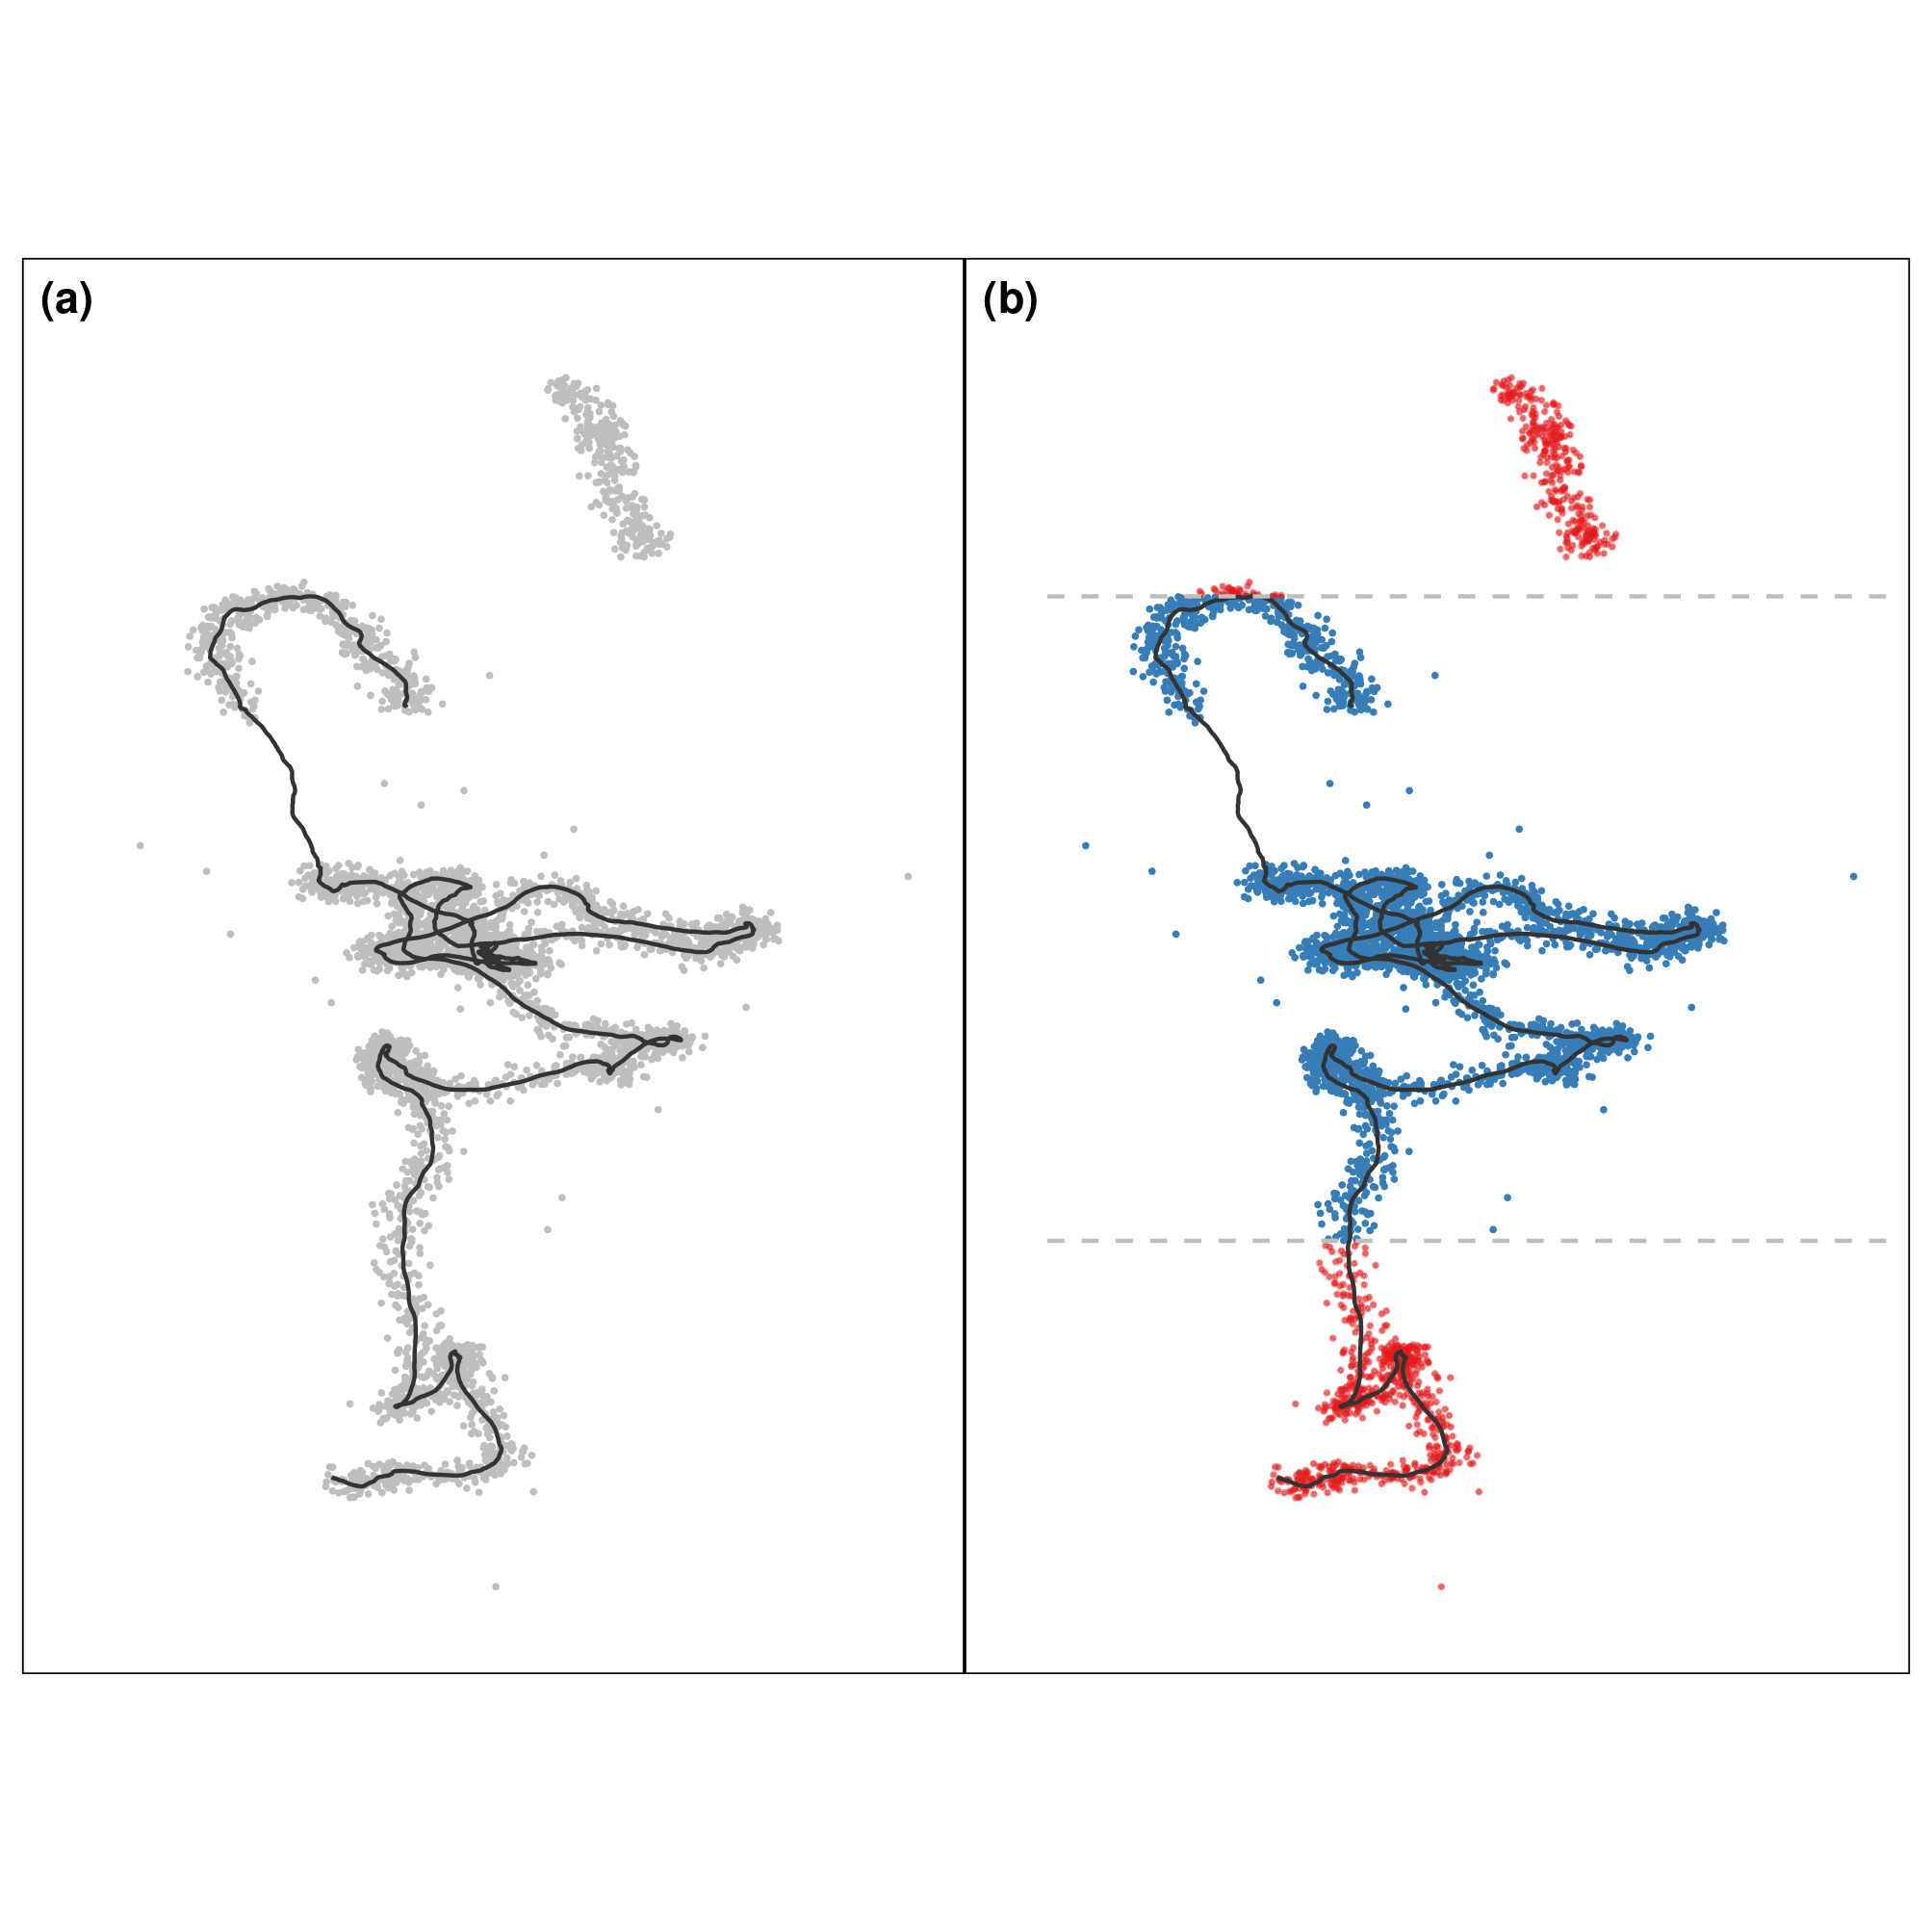
\includegraphics{figures/fig_raw_bounds.png}

\textbf{(a)} A velocity-autocorrelated movement track simulated for 5,000 positions (black line) using the \texttt{smoove} package (Gurarie et al.~2017). Three kinds of errors have been artificially added: (1) each position (grey points) is offset from the canonical track with the addition of normally distributed small-scale error, (2) large-scale error has been added to 0.5\% of positions, and (3) 300 positions (indices 500 -- 800) have been displaced to the top-right of the track to simulate a gross distortion that affects a continuous subset of the track.
The goal of pre-processing such datasets is to get the estimated positions (grey points) to match the canonical track (solid black line) as closely as possible.
\textbf{(b)} Tracks can be quickly filtered by spatial bounds (\(0.5 \leq Y \leq 1.0\); dashed grey lines) using the \texttt{atlastools} function \texttt{atl\_filter\_bounds}. Setting the function argument \texttt{remove\_inside\ =\ FALSE} retains positions within user supplied bounds (blue points), and excludes those outside (red points).

\hypertarget{a-note-on-filtering-by-bounds}{%
\subsection{A Note on Filtering by Bounds}\label{a-note-on-filtering-by-bounds}}

The filter on spatial bounds is only for demonstration, and is not applied to the data.

\hypertarget{filtering-unrealistic-movement}{%
\section{Filtering Unrealistic Movement}\label{filtering-unrealistic-movement}}

Large-scale positioning error can affect both point locations as well as entire subsets of a track, leading to a track appearing to show unrealistic movement for the study species (Bjørneraas et al. \protect\hyperlink{ref-bjorneraas2010}{2010}).

The best way to examine whether a track contains such positioning errors is to plot the data, and especially to join the dots, i.e., to connect the positions with lines rather than simply plot points.

Users with extensive experience of their study system will readily recognise segments of a track where the movement appears to be unrealistic.

Briefly, the two main kinds of errors are mentioned here, and named based on their appearance in a tack: those that affect single positions lend a spiky appearance to a track, and are referred to as \emph{point outliers} or \emph{spikes}, while errors affecting continuous subsets of a track cause it to appear as though it has been reflected along a plane, and are hence called \emph{reflections}, or \emph{prolonged spikes}.

\hypertarget{filtering-point-outliers-or-spikes}{%
\subsection{Filtering Point Outliers or Spikes}\label{filtering-point-outliers-or-spikes}}

We begin by removing unrealistic movement in the form of point outliers, or spikes.

The first step is to determine how spikes should be identified. The non-movement approach prescribes determining whether movement metrics associated with each position are realistic or not, and targeting those positions where the movement metrics are unrealistic for the study species.

In this case we shall calculate only two metrics, speed and turning angle.
These are conveniently implemented in \texttt{atlastools} using the functions \texttt{atl\_get\_speed} and \texttt{atl\_turning\_angle}.

\begin{Shaded}
\begin{Highlighting}[]
\CommentTok{\# get speed and turning angle}
\NormalTok{data\_copy[, }\StringTok{\textasciigrave{}}\DataTypeTok{:=}\StringTok{\textasciigrave{}}\NormalTok{(}\DataTypeTok{in\_speed =} \KeywordTok{atl\_get\_speed}\NormalTok{(data\_copy,}
                                          \DataTypeTok{type =} \StringTok{"in"}\NormalTok{),}
                 \DataTypeTok{out\_speed =} \KeywordTok{atl\_get\_speed}\NormalTok{(data\_copy,}
                                           \DataTypeTok{type =} \StringTok{"out"}\NormalTok{),}
                 \DataTypeTok{angle =} \KeywordTok{atl\_turning\_angle}\NormalTok{(data\_copy))]}
\end{Highlighting}
\end{Shaded}

Having calculated speed and turning angle, the next step is to remove positions with extremely high incoming and outgoing speeds. This means using the \texttt{atl\_filter\_covariates} function to remove positions with speed \(\geq\) a plausible speed threshold. The use of a turning angle filter is optional, and not necessary in this case.

One approach is to define a speed cutoff based on expert knowledge, and this is best suited to well studied species.

For simulated data, there is no plausible speed threshold from prior knowledge --- a reasonable choice here is to use the 90\^{}th or 95\^{}th percentile of speed and turning angle (when this metric is used).

This is also more general than identifying the limits of implausibility for each individual (since there may be inter-individual differences), let alone each species in a large dataset.

\begin{Shaded}
\begin{Highlighting}[]
\CommentTok{\# get 90 and 95 percentile of speed and turning angle}
\KeywordTok{sapply}\NormalTok{(data\_copy[, }\KeywordTok{c}\NormalTok{(}\StringTok{"in\_speed"}\NormalTok{, }\StringTok{"angle"}\NormalTok{)], }\ControlFlowTok{function}\NormalTok{(z) \{}
  \KeywordTok{quantile}\NormalTok{(z, }\DataTypeTok{probs =} \KeywordTok{c}\NormalTok{(}\FloatTok{0.9}\NormalTok{, }\FloatTok{0.95}\NormalTok{), }\DataTypeTok{na.rm =} \OtherTok{TRUE}\NormalTok{)}
\NormalTok{\})}
\end{Highlighting}
\end{Shaded}

Finally, we shall remove positions whose incoming and outgoing speeds are both greater than the 95th speed percentile using \texttt{atl\_filter\_covariates}.

\begin{Shaded}
\begin{Highlighting}[]
\CommentTok{\# filter the copy by the 95th percentile}
\NormalTok{data\_filtered <{-}}\StringTok{ }\KeywordTok{atl\_filter\_covariates}\NormalTok{(data\_copy,}
    \DataTypeTok{filters =} \KeywordTok{c}\NormalTok{(}\StringTok{"(in\_speed < 0.024 \& out\_speed < 0.024) | angle < 40"}\NormalTok{))}
\end{Highlighting}
\end{Shaded}

We prepare the data for plotting.

\hypertarget{filtering-reflections-or-track-subsets}{%
\subsection{Filtering Reflections or Track Subsets}\label{filtering-reflections-or-track-subsets}}

When entire track subsets are affected by positioning error, they are more difficult to remove. This is the case when positions are \emph{reflected} along a plane in the coordinate axis --- the simplest way in which this can be explained is to examine the way in which we simulated the reflection earlier in this text, by simply adding an offset to the X and Y coordinates of each of 300 consecutive positions (indices 500 -- 800).

An explanation of why these reflections occur is found in WATLAS PAPER: Bijleveld et al.~in prep. In short, they are results of an error in the ATLAS localisation algorithm, and are usually removed in the localisation step's quality control procedures. However, some reflections may remain to confront users.

Reflections and other issues affecting track subsets cannot be resolved by targeting single positions, since there are rarely any position-specific covariates that can be used to identify a position as part of a larger subset that should be removed.

However, it is often possible to identify the \emph{bounds} of problematic subsets, such as reflections, and remove positions between them. The way this is done is conceptually similar to the point outlier algorithm.

The \texttt{atl\_remove\_reflection} function implements one method remove reflected subsets of a track. The working is described:

\begin{enumerate}
\def\labelenumi{\arabic{enumi}.}
\item
  Remove point outliers,
\item
  Re-calculate speed and turning angles
\item
  Identify the first unrealistic movement position (fast speed and high turning angle)
\item
  Setting this point as an anchor, identify the next position with unrealistic movement (as above)
\item
  Remove all positions between these two points,
\item
  Search for the next unrealistic movement, and repeat the process.
\end{enumerate}

This is a minimal algorithm which can be developed further, and iterated multiple times to comprehensively remove reflections.

One important function argument is the estimated reflection length, i.e., how many positions are estimated to be reflected. This argument controls how many positions after the anchor are candidates for the reflection's end.

If the reflection does not end within this number of positions, the algorithm goes awry, and considers part of the reflection to be the valid data.
Fortunately, this can be avoided by setting the length to the number of observations in the data.

However, if the reflection does not end at all, the algorithm will simply delete all positions from the anchor point onwards.

Thus, the algorithm is less of a double-edged sword and more a sword with no hilt --- there are few safe ways to use it.

The difficulty in implementing a reasonable algorithm for dealing with this kind of track-subset wide positioning error reveals the general problem that algorithms are \textbf{not} easy to conceptualise or efficiently implement.

\begin{Shaded}
\begin{Highlighting}[]
\CommentTok{\# attempt to remove reflections}
\NormalTok{data\_no\_reflection <{-}}\StringTok{ }\KeywordTok{atl\_remove\_reflections}\NormalTok{(data\_filtered,}
                          \DataTypeTok{point\_angle\_cutoff =} \DecValTok{10}\NormalTok{,}
                          \DataTypeTok{reflection\_speed\_cutoff =} \FloatTok{0.024}\NormalTok{)}
\CommentTok{\# get reflections}
\NormalTok{reflection <{-}}\StringTok{ }\NormalTok{data\_filtered[}\OperatorTok{!}\NormalTok{data\_no\_reflection,}
\NormalTok{                                         on =}\StringTok{ }\KeywordTok{c}\NormalTok{(}\StringTok{"x"}\NormalTok{, }\StringTok{"y"}\NormalTok{)]}
\NormalTok{reflection <{-}}\StringTok{ }\KeywordTok{na.omit}\NormalTok{(reflection)}
\end{Highlighting}
\end{Shaded}

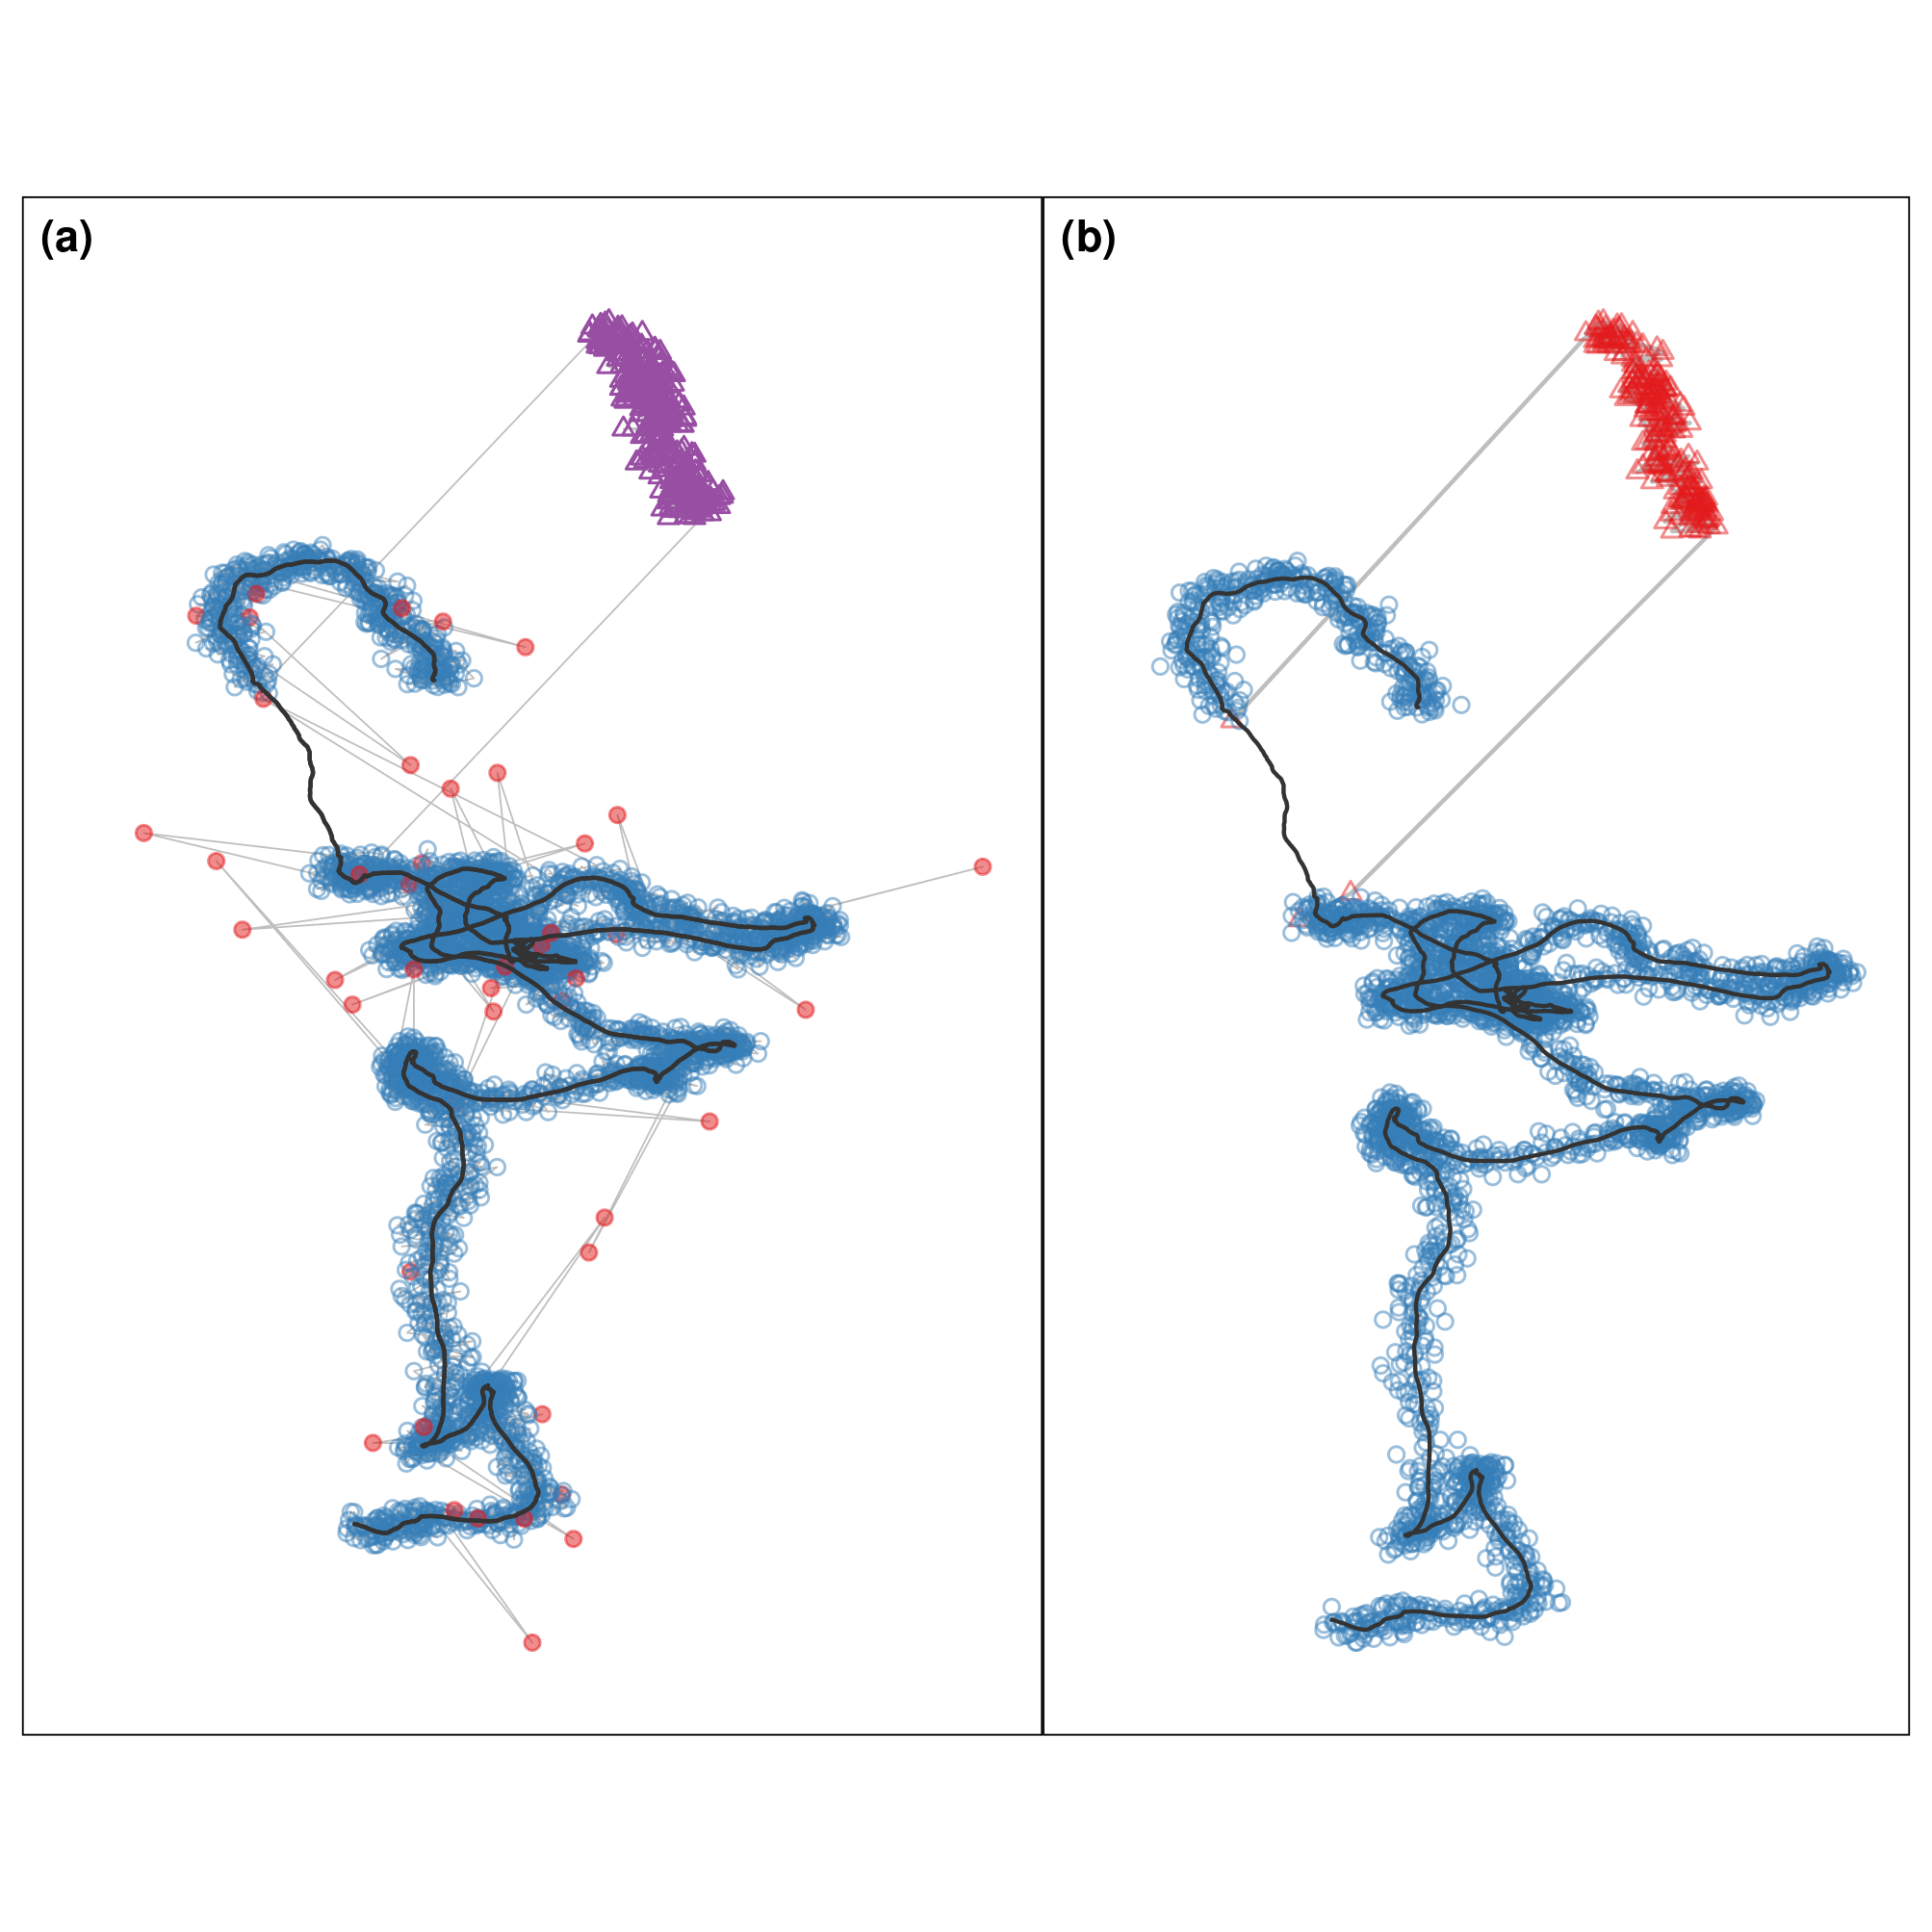
\includegraphics{figures/fig_correct_tracks.png}

Reducing large-scale positioning error in a movement track. \textbf{(a)} Positioning error may affect single observations resulting in point outliers or `spikes' (red points), but it may also affect continuous susbets of a track, which we call a \texttt{prolonged\ spike\textquotesingle{}\ (purple\ triangles).\ While\ the\ former\ may\ be\ targeted\ by\ filtering\ on\ appropriate\ covariates\ such\ as\ speed\ and\ turning\ angle\ using\ the}atlastools\texttt{function}atl\_filter\_covariates\texttt{,\ the\ latter\ cannot\ be\ effectively\ corrected\ by\ targeting\ each\ coordinate\ pair\ in\ isolation.\ **(b)**\ The}atlastools\texttt{function}atl\_remove\_reflections` to identify prolonged spikes (red triangles) in tracking data is an illustrative example of targeting positioning errors that affect track subsets. While this method returns the canonical track without the prolonged spike (blue points) in this example, users are cautioned to frequently check this and similar semi-supervised algorithms' results.

Finally, we export the data without spikes and reflections to be used later.

\begin{Shaded}
\begin{Highlighting}[]
\KeywordTok{fwrite}\NormalTok{(data\_no\_reflection, }\DataTypeTok{file =} \StringTok{"data/data\_no\_reflection.csv"}\NormalTok{)}
\end{Highlighting}
\end{Shaded}

\hypertarget{reducing-small-scale-positioning-error-and-aggregating-data}{%
\chapter{Reducing Small-Scale Positioning Error and Aggregating Data}\label{reducing-small-scale-positioning-error-and-aggregating-data}}

Once large-scale positioning errors have been removed using filters on bounds or on unrealistic movement, small-scale positioning errors may remain. Why is this the case?

The simple reason is that high-frequency tracking has a large component of error relative to the real movement of an individual, and the error / movement ratio increases with the frequency of tracking. (Noonan et al. \protect\hyperlink{ref-noonan2019}{2019}) has a better explanation, which users are strongly recommended to read.

The effect of these small-scale errors for high-frequency data is to cause overestimations of straight-line displacement (distance between two positions) and speed. If users were to apply a very strict speed filter, many of these positions would be lost. This loss of information would certainly reduce the sampling frequency, which would lead to better estimates of total distance and mean speed. However, while \emph{total} distance and \emph{mean} speed estimates would improve, the instantaneous distance and speed estimates would remain biased, which will most likely lead to erroneous inferences from the data.

However, users can turn the high-frequency of their data against itself by applying a simple smooth. The median smooth is recommended because it is robust to outliers, and is very well understood.

\hypertarget{preparing-libraries-and-data}{%
\section{Preparing Libraries and Data}\label{preparing-libraries-and-data}}

We first load some useful packages and define a colour palette.

\begin{Shaded}
\begin{Highlighting}[]
\CommentTok{\# prep libs}
\KeywordTok{library}\NormalTok{(data.table)}
\KeywordTok{library}\NormalTok{(atlastools)}
\KeywordTok{library}\NormalTok{(ggplot2)}
\KeywordTok{library}\NormalTok{(patchwork)}

\CommentTok{\# prepare a palette}
\NormalTok{pal <{-}}\StringTok{ }\NormalTok{RColorBrewer}\OperatorTok{::}\KeywordTok{brewer.pal}\NormalTok{(}\DecValTok{4}\NormalTok{, }\StringTok{"Set1"}\NormalTok{)}
\end{Highlighting}
\end{Shaded}

We load both the simulated, canonical data (which has no errors), as well as the data with errors which has been pre-processed to remove large-scale errors.

We also assign a variable, \texttt{window\_size}, which will help identify the datasets when comparing median smooth moving window (\(K\)) sizes.

\begin{Shaded}
\begin{Highlighting}[]
\CommentTok{\# read in the data and set the window size variable}
\NormalTok{data <{-}}\StringTok{ }\KeywordTok{fread}\NormalTok{(}\StringTok{"data/data\_sim.csv"}\NormalTok{)[}\DecValTok{5000}\OperatorTok{:}\DecValTok{10000}\NormalTok{, ]}
\NormalTok{data[, window\_size }\OperatorTok{:}\ErrorTok{=}\StringTok{ }\OtherTok{NA}\NormalTok{]}

\CommentTok{\# data with small scale errors but no reflections or outliers}
\NormalTok{data\_errors <{-}}\StringTok{ }\KeywordTok{fread}\NormalTok{(}\StringTok{"data/data\_no\_reflection.csv"}\NormalTok{)}
\NormalTok{data\_errors[, window\_size }\OperatorTok{:}\ErrorTok{=}\StringTok{ }\DecValTok{0}\NormalTok{]}
\end{Highlighting}
\end{Shaded}

\hypertarget{median-smoothing}{%
\section{Median Smoothing}\label{median-smoothing}}

We apply a median smooth with four different values of \(K\), the moving window size --- 3, 5, 11, and 21 positions.
\(K\) must be an odd number, but apart from that there is no correct magnitude of \(K\).
Very large \(K\) will lead to unrealistic tracks, while small \(K\) will not result in much reduction of error.
Users are encouraged to plot their data before and after smoothing to examine the effect of different window sizes.

The \texttt{atlastools} function \texttt{atl\_median\_smooth} is quite fast and users can readily try multiple \(K\) values as shown in the example below.

\begin{Shaded}
\begin{Highlighting}[]
\CommentTok{\# smooth the data over four K values}
\NormalTok{list\_of\_smooths <{-}}\StringTok{ }\KeywordTok{lapply}\NormalTok{(}\KeywordTok{c}\NormalTok{(}\DecValTok{3}\NormalTok{, }\DecValTok{5}\NormalTok{, }\DecValTok{11}\NormalTok{, }\DecValTok{21}\NormalTok{), }\ControlFlowTok{function}\NormalTok{(K) \{}
  
\NormalTok{  data\_copy <{-}}\StringTok{ }\KeywordTok{copy}\NormalTok{(data\_errors)}
  
\NormalTok{  data\_copy <{-}}\StringTok{ }\KeywordTok{atl\_median\_smooth}\NormalTok{(}\DataTypeTok{data =}\NormalTok{ data\_copy,}
                    \DataTypeTok{x =} \StringTok{"x"}\NormalTok{, }
                    \DataTypeTok{y =} \StringTok{"y"}\NormalTok{,}
                    \DataTypeTok{time =} \StringTok{"time"}\NormalTok{,}
                    \DataTypeTok{moving\_window =}\NormalTok{ K)}
  
\NormalTok{  data\_copy[, window\_size }\OperatorTok{:}\ErrorTok{=}\StringTok{ }\NormalTok{K]}
\NormalTok{\})}
\end{Highlighting}
\end{Shaded}

We save the 11 point smoothed data.

\begin{Shaded}
\begin{Highlighting}[]
\KeywordTok{fwrite}\NormalTok{(list\_of\_smooths[[}\DecValTok{3}\NormalTok{]], }\DataTypeTok{file =} \StringTok{"data/data\_smooth.csv"}\NormalTok{)}
\end{Highlighting}
\end{Shaded}

We prepare the data for plotting.

\begin{Shaded}
\begin{Highlighting}[]
\CommentTok{\# bind list after offset}
\NormalTok{data\_plot <{-}}\StringTok{ }\KeywordTok{mapply}\NormalTok{(}\ControlFlowTok{function}\NormalTok{(df, offset) \{}
\NormalTok{  df[, x }\OperatorTok{:}\ErrorTok{=}\StringTok{ }\NormalTok{x }\OperatorTok{+}\StringTok{ }\NormalTok{offset]}
\NormalTok{\}, list\_of\_smooths, }\KeywordTok{seq}\NormalTok{(}\FloatTok{0.4}\NormalTok{, }\FloatTok{1.25}\NormalTok{, }\DataTypeTok{length.out =} \DecValTok{4}\NormalTok{),}
\DataTypeTok{SIMPLIFY =}\NormalTok{ F)}

\NormalTok{data\_plot <{-}}\StringTok{ }\KeywordTok{rbindlist}\NormalTok{(data\_plot)}
\end{Highlighting}
\end{Shaded}

We prepare a plot of the smoothed data.

\hypertarget{thinning-data-by-aggregation}{%
\section{Thinning Data by Aggregation}\label{thinning-data-by-aggregation}}

Evenly thinning data is a good idea if statistical methods require even sampling, or if the volume of data is too large for statistical packages to efficiently handle it. In \texttt{R}, both may be true at once.

Here, we demonstrate thinning by aggregation on data that has been median smoothed using a \(K\) of 11.

\begin{Shaded}
\begin{Highlighting}[]
\CommentTok{\# choose the 11 point median smooth data}
\NormalTok{data\_agg <{-}}\StringTok{ }\KeywordTok{copy}\NormalTok{(list\_of\_smooths[[}\DecValTok{3}\NormalTok{]])}

\CommentTok{\# get list of aggregated data}
\NormalTok{list\_of\_agg <{-}}\StringTok{ }\KeywordTok{lapply}\NormalTok{(}\KeywordTok{c}\NormalTok{(}\DecValTok{3}\NormalTok{, }\DecValTok{10}\NormalTok{, }\DecValTok{30}\NormalTok{, }\DecValTok{120}\NormalTok{), }\ControlFlowTok{function}\NormalTok{(z) \{}
  
\NormalTok{  data\_return <{-}}\StringTok{ }\KeywordTok{atl\_thin\_data}\NormalTok{(}\DataTypeTok{data =}\NormalTok{ data\_agg,}
                            \DataTypeTok{interval =}\NormalTok{ z,}
                            \DataTypeTok{method =} \StringTok{"aggregate"}\NormalTok{)}
  
\NormalTok{  data\_return[, interval }\OperatorTok{:}\ErrorTok{=}\StringTok{ }\NormalTok{z]}
  
  \KeywordTok{return}\NormalTok{(data\_return)}
\NormalTok{\})}

\CommentTok{\# get mean speed estimate and sd}
\NormalTok{speed\_agg\_smooth <{-}}\StringTok{ }
\StringTok{  }\KeywordTok{lapply}\NormalTok{(list\_of\_agg, }\ControlFlowTok{function}\NormalTok{(df) \{}
    \KeywordTok{na.omit}\NormalTok{(df)}
\NormalTok{    df[, speed }\OperatorTok{:}\ErrorTok{=}\StringTok{ }\KeywordTok{atl\_get\_speed}\NormalTok{(df)]}
\NormalTok{    df[, }\KeywordTok{list}\NormalTok{(}\DataTypeTok{median =} \KeywordTok{median}\NormalTok{(speed, }\DataTypeTok{na.rm =}\NormalTok{ T),}
              \DataTypeTok{sd =} \KeywordTok{sd}\NormalTok{(speed, }\DataTypeTok{na.rm =}\NormalTok{ T),}
              \DataTypeTok{interval =} \KeywordTok{first}\NormalTok{(interval))]}
\NormalTok{  \})}

\CommentTok{\# bind}
\NormalTok{speed\_agg\_smooth <{-}}\StringTok{ }\KeywordTok{rbindlist}\NormalTok{(speed\_agg\_smooth)}
\end{Highlighting}
\end{Shaded}

\hypertarget{aggregation-before-reducing-positioning-errors}{%
\section{Aggregation Before Reducing Positioning Errors}\label{aggregation-before-reducing-positioning-errors}}

Users may rightly wonder whether they can get away with aggregating their data, using a median aggregation function, and reduce data volumes, correct uneven sampling frequency, and reduce large-scale errors all in one go.

The answer to most questions in ecology is, ``It depends''. Median aggregation before correcting positioning errors can indeed be advantageous; for instance for faster visualisation while preserving the broad structure of a track.

However, there are drawbacks. The main one is that information is lost in the aggregation process, lending less power to steps such as smoothing applied after aggregation.
Further, aggregation (and indeed any kind of thinning) results in significantly different estimates of speed and distance from the real speed.

We show the effect of aggregating before any error correction here.

\begin{Shaded}
\begin{Highlighting}[]
\CommentTok{\# read data with errors}
\NormalTok{data\_errors <{-}}\StringTok{ }\KeywordTok{fread}\NormalTok{(}\StringTok{"data/data\_errors.csv"}\NormalTok{)}
  
\CommentTok{\# aggregate before correction}
\NormalTok{list\_of\_agg <{-}}\StringTok{ }\KeywordTok{lapply}\NormalTok{(}\KeywordTok{c}\NormalTok{(}\DecValTok{3}\NormalTok{, }\DecValTok{10}\NormalTok{, }\DecValTok{30}\NormalTok{, }\DecValTok{120}\NormalTok{), }\ControlFlowTok{function}\NormalTok{(z) \{}
\NormalTok{  data\_return <{-}}\StringTok{ }\KeywordTok{atl\_thin\_data}\NormalTok{(}\DataTypeTok{data =}\NormalTok{ data\_errors,}
                            \DataTypeTok{interval =}\NormalTok{ z,}
                            \DataTypeTok{method =} \StringTok{"aggregate"}\NormalTok{)}
\NormalTok{  data\_return[, interval }\OperatorTok{:}\ErrorTok{=}\StringTok{ }\NormalTok{z]}
\NormalTok{  data\_return[, speed }\OperatorTok{:}\ErrorTok{=}\StringTok{ }\KeywordTok{atl\_get\_speed}\NormalTok{(data\_return)]}
  \KeywordTok{return}\NormalTok{(data\_return)}
\NormalTok{\})}

\CommentTok{\# get real speed}
\NormalTok{data[, speed }\OperatorTok{:}\ErrorTok{=}\StringTok{ }\KeywordTok{atl\_get\_speed}\NormalTok{(data)]}
\end{Highlighting}
\end{Shaded}

\hypertarget{comparing-median-aggregation-with-and-without-smoothing}{%
\subsection{Comparing median aggregation with and without smoothing}\label{comparing-median-aggregation-with-and-without-smoothing}}

\begin{Shaded}
\begin{Highlighting}[]
\CommentTok{\# now plot distribution of speed}
\NormalTok{data\_agg <{-}}\StringTok{ }\KeywordTok{rbindlist}\NormalTok{(list\_of\_agg)}
\end{Highlighting}
\end{Shaded}

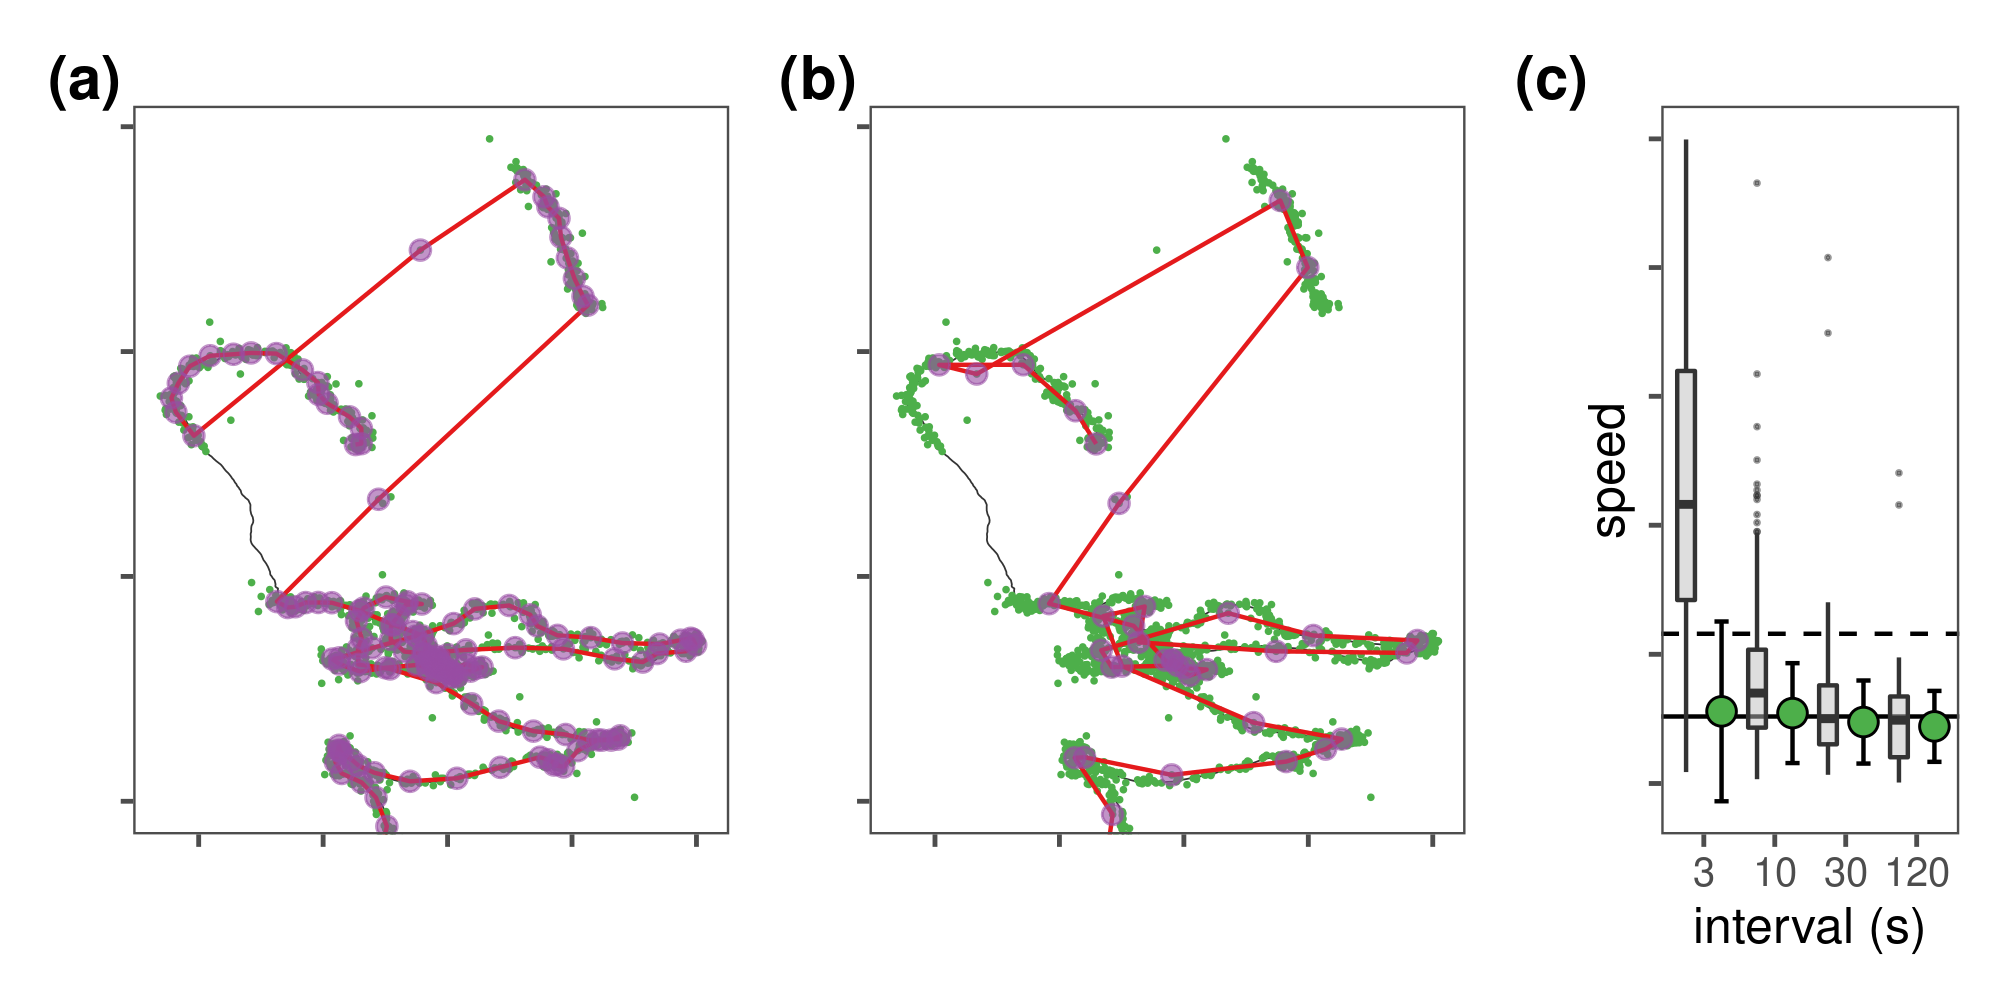
\includegraphics{figures/fig_aggregate_errors.png}

Thinning a movement track using median aggregation preserves track structure, but affects essential track metrics such as speed.
\textbf{(a, b)} Movement tracks with a canonical interval of 1s aggregated over intervals of \textbf{(a)} 10 and \textbf{(b)} 30 seconds, without removing large- or small-scale positioning errors. All symbols represent positions in the aggregated track, with the size of the symbol representing the standard deviation at each position.
Blue crosses represent positions with speed \(\leq\) the 95\^{}th percentile of canonical speeds, while red triangles represent positions with speed \(\geq\) 95\^{}th percentile of canonical speeds.
\textbf{(c)} Boxplot of instantaneous speeds after median aggregation of a 1s interval track over intervals of 3, 10, 30, and 120 seconds, but without the removal of positioning errors. The mean and 95\^{}th percentile of speed in the canonical track are shown as solid and dashed lines, respectively.
Aggregation without reducing positioning errors can result in speed estimates that are substantially different from the true speed.

\hypertarget{residence-patches-and-their-construction}{%
\chapter{Residence patches and their construction}\label{residence-patches-and-their-construction}}

\hypertarget{prepare-libraries}{%
\section*{Prepare libraries}\label{prepare-libraries}}
\addcontentsline{toc}{section}{Prepare libraries}

\begin{Shaded}
\begin{Highlighting}[]
\KeywordTok{library}\NormalTok{(data.table)}
\KeywordTok{library}\NormalTok{(atlastools)}
\KeywordTok{library}\NormalTok{(ggplot2)}
\KeywordTok{library}\NormalTok{(patchwork)}

\CommentTok{\# for residence time}
\KeywordTok{library}\NormalTok{(recurse)}

\CommentTok{\# prepare a palette}
\NormalTok{pal <{-}}\StringTok{ }\NormalTok{RColorBrewer}\OperatorTok{::}\KeywordTok{brewer.pal}\NormalTok{(}\DecValTok{4}\NormalTok{, }\StringTok{"Set1"}\NormalTok{)}
\end{Highlighting}
\end{Shaded}

\hypertarget{an-example-with-simulated-data}{%
\section{An example with simulated data}\label{an-example-with-simulated-data}}

\hypertarget{read-data-and-classify}{%
\subsection{Read data and classify}\label{read-data-and-classify}}

\begin{Shaded}
\begin{Highlighting}[]
\CommentTok{\# read patch data}
\NormalTok{data <{-}}\StringTok{ }\KeywordTok{fread}\NormalTok{(}\StringTok{"data/data\_for\_res\_patch.csv"}\NormalTok{)}

\CommentTok{\# filter}
\NormalTok{data <{-}}\StringTok{ }\NormalTok{data[y }\OperatorTok{<}\StringTok{ }\DecValTok{21}\NormalTok{, ]}

\CommentTok{\# do recurse}
\NormalTok{data\_recurse <{-}}\StringTok{ }\KeywordTok{getRecursions}\NormalTok{(data[, }\KeywordTok{list}\NormalTok{(x, y, time, id)],}
                              \DataTypeTok{radius =} \DecValTok{1}\NormalTok{)}

\CommentTok{\# assign residence time}
\NormalTok{data[, residence\_time }\OperatorTok{:}\ErrorTok{=}\StringTok{ }\NormalTok{data\_recurse}\OperatorTok{$}\NormalTok{residenceTime]}
\end{Highlighting}
\end{Shaded}

We first plot a figure of residence time per positions, and residence time per timestamp.

We construct residence patches from data where residence time is \textgreater{} 0.15.

\begin{Shaded}
\begin{Highlighting}[]
\CommentTok{\# make residence patch}
\NormalTok{patch <{-}}\StringTok{ }\KeywordTok{atl\_res\_patch}\NormalTok{(data[residence\_time }\OperatorTok{>}\StringTok{ }\FloatTok{0.04}\NormalTok{, ], }
                       \DataTypeTok{buffer\_radius =} \FloatTok{0.1}\NormalTok{, }
                       \DataTypeTok{lim\_spat\_indep =} \DecValTok{1}\NormalTok{, }
                       \DataTypeTok{lim\_time\_indep =} \DecValTok{30}\NormalTok{)}



\CommentTok{\# get spatial representation}
\NormalTok{patch\_sf <{-}}\StringTok{ }\KeywordTok{atl\_patch\_summary}\NormalTok{(}\DataTypeTok{patch\_data =}\NormalTok{ patch,}
                              \DataTypeTok{which\_data =} \StringTok{"spatial"}\NormalTok{, }
                              \DataTypeTok{buffer\_radius =} \FloatTok{0.15}\NormalTok{)}

\CommentTok{\# get summary data}
\NormalTok{patch\_summary <{-}}\StringTok{ }\KeywordTok{atl\_patch\_summary}\NormalTok{(}\DataTypeTok{patch\_data =}\NormalTok{ patch,}
                                   \DataTypeTok{which\_data =} \StringTok{"summary"}\NormalTok{)}
\end{Highlighting}
\end{Shaded}

\hypertarget{plot-classified-residence-patches}{%
\subsection{Plot classified residence patches}\label{plot-classified-residence-patches}}

We arrange the figures together.

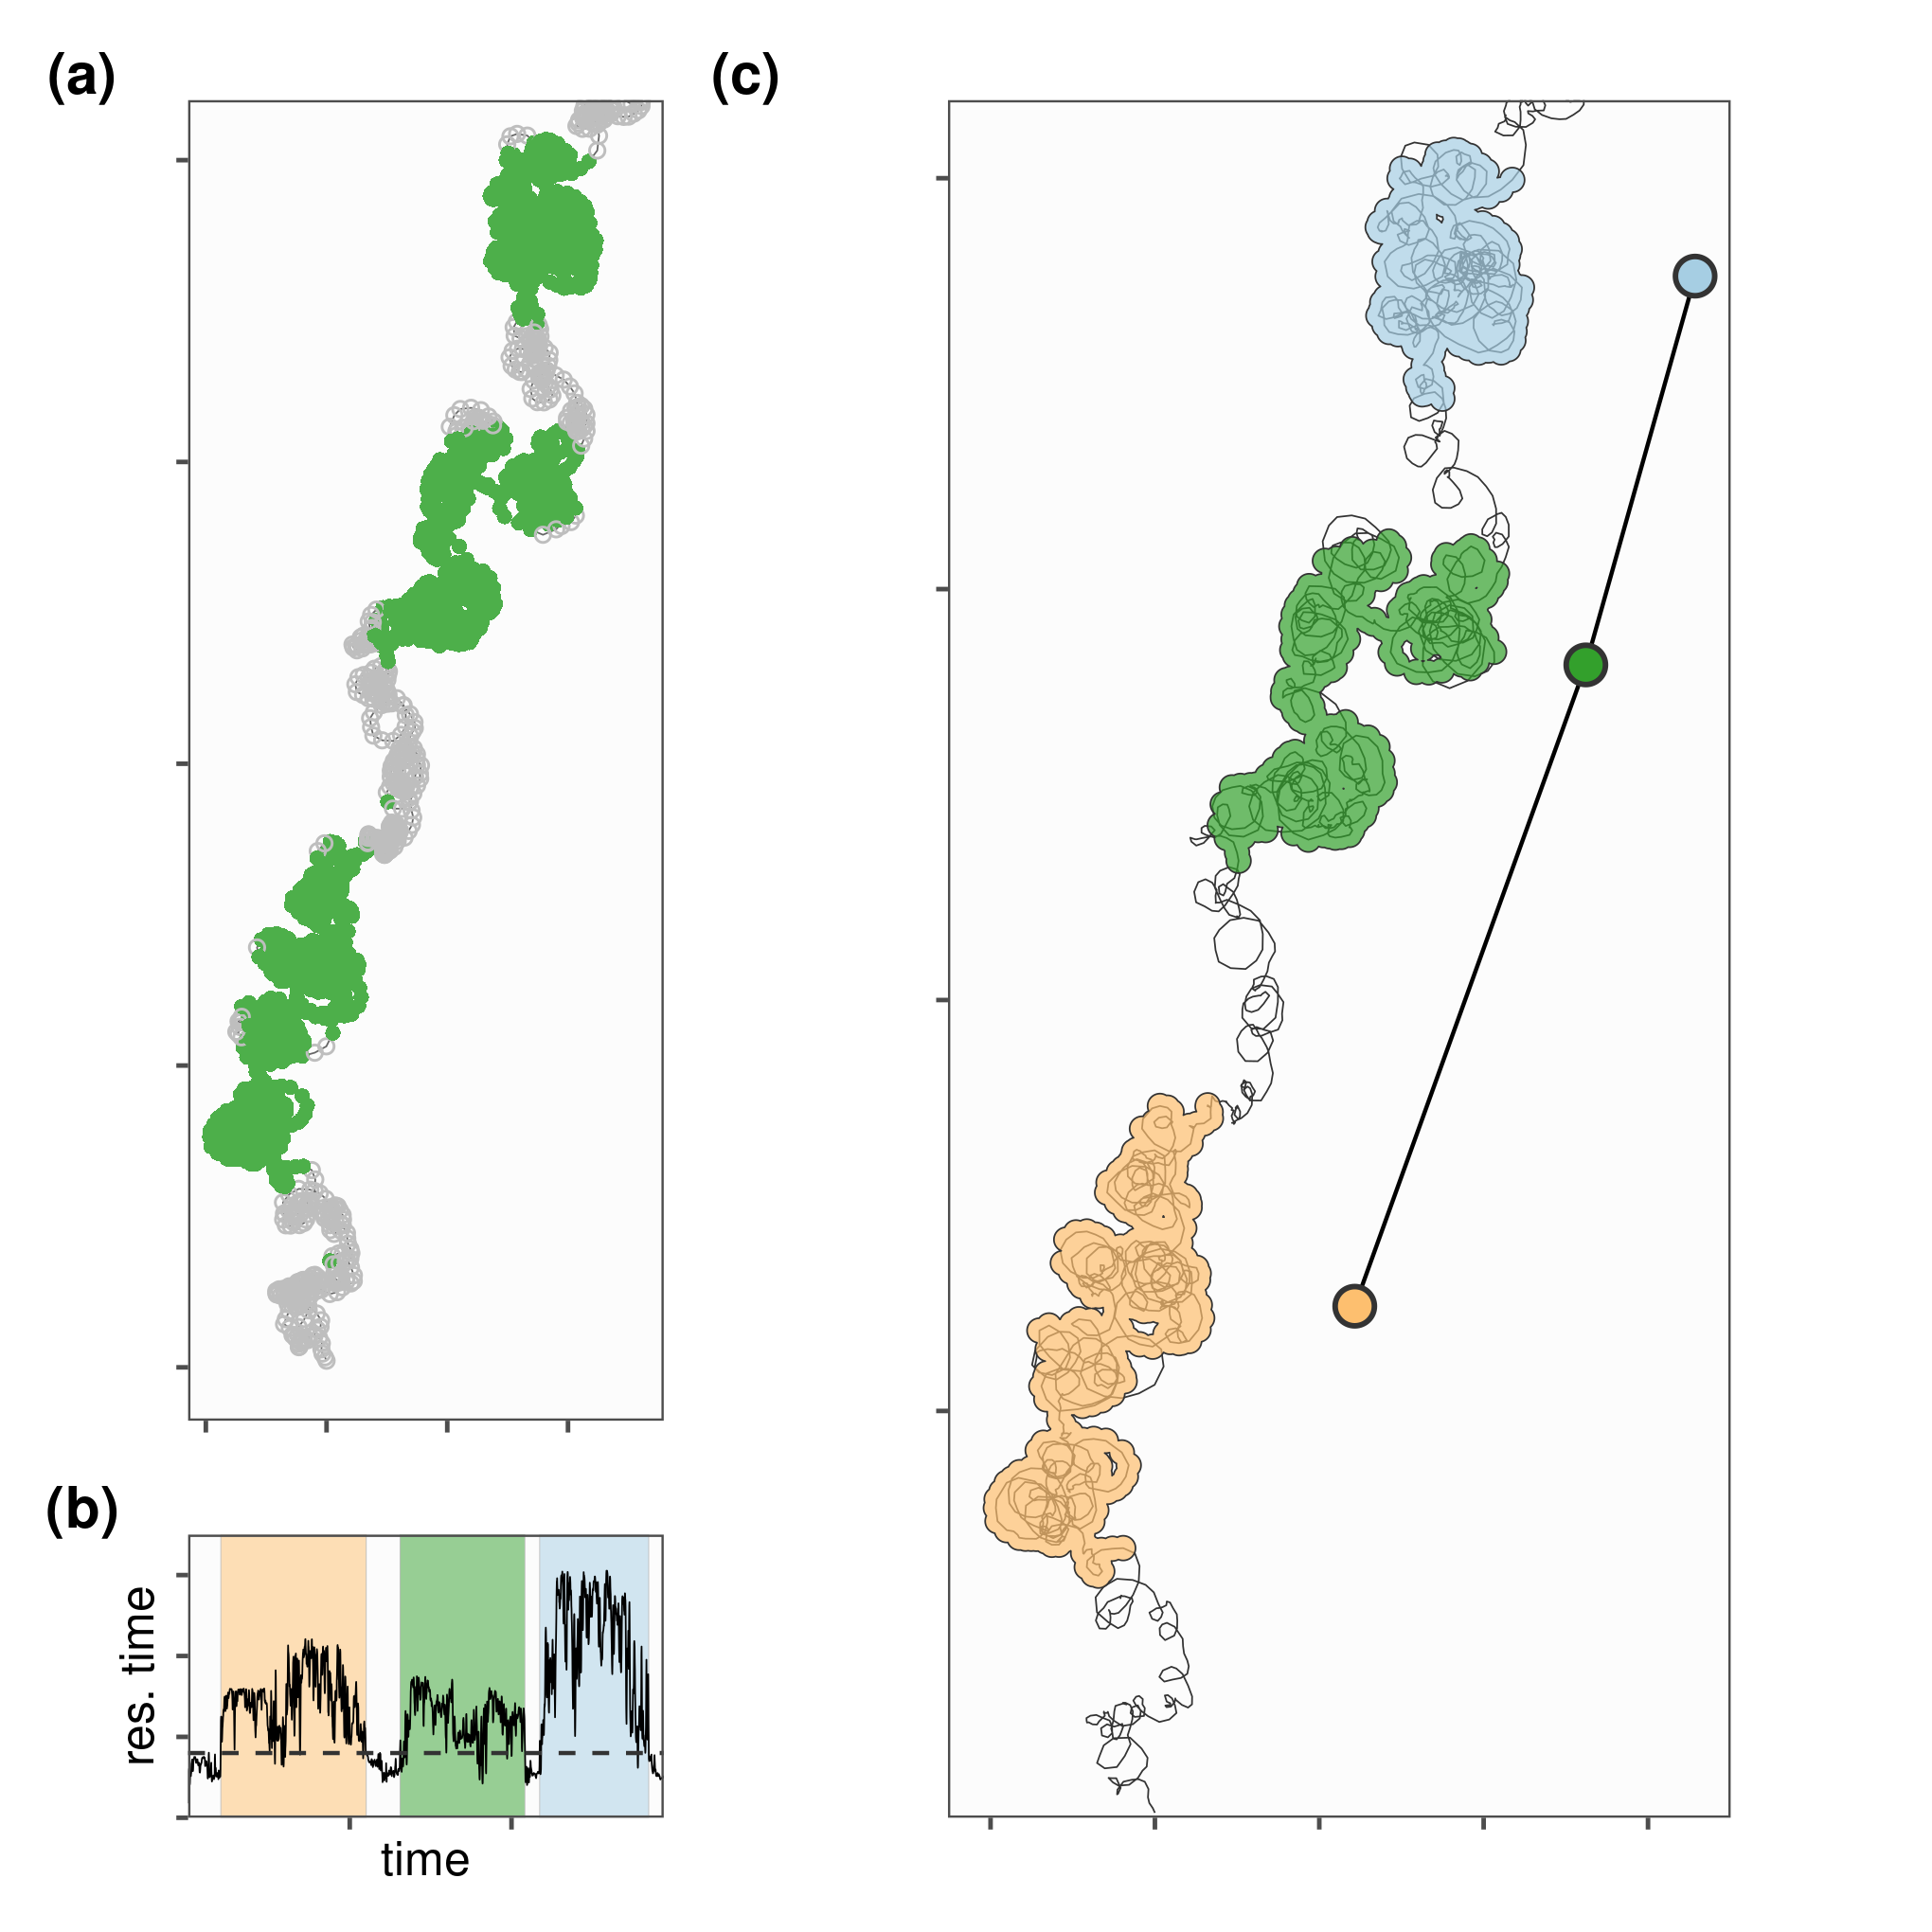
\includegraphics{figures/fig_residence.png}

\hypertarget{processing-calibration-data}{%
\chapter{Processing calibration data}\label{processing-calibration-data}}

\hypertarget{prepare-libraries}{%
\section{Prepare libraries}\label{prepare-libraries}}

\begin{Shaded}
\begin{Highlighting}[]
\CommentTok{\# load libs}
\KeywordTok{library}\NormalTok{(data.table)}
\KeywordTok{library}\NormalTok{(atlastools)}
\KeywordTok{library}\NormalTok{(ggplot2)}
\KeywordTok{library}\NormalTok{(patchwork)}

\CommentTok{\# prepare a palette}
\NormalTok{pal <{-}}\StringTok{ }\NormalTok{RColorBrewer}\OperatorTok{::}\KeywordTok{brewer.pal}\NormalTok{(}\DecValTok{4}\NormalTok{, }\StringTok{"Set1"}\NormalTok{)}
\end{Highlighting}
\end{Shaded}

\hypertarget{preliminary-visualisation}{%
\section{Preliminary visualisation}\label{preliminary-visualisation}}

\begin{Shaded}
\begin{Highlighting}[]
\CommentTok{\# read and plot example data}
\NormalTok{data <{-}}\StringTok{ }\KeywordTok{fread}\NormalTok{(}\StringTok{"data/atlas1060\_allTrials\_annotated.csv"}\NormalTok{)}
\NormalTok{data\_raw <{-}}\StringTok{ }\KeywordTok{copy}\NormalTok{(data)}
\end{Highlighting}
\end{Shaded}

\hypertarget{filter-by-bounding-box}{%
\section{Filter by bounding box}\label{filter-by-bounding-box}}

Save an unprocessed copy.

\begin{Shaded}
\begin{Highlighting}[]
\NormalTok{data\_unproc <{-}}\StringTok{ }\KeywordTok{copy}\NormalTok{(data)}
\end{Highlighting}
\end{Shaded}

Filter by a bounding box.

\begin{Shaded}
\begin{Highlighting}[]
\CommentTok{\# remove inside must be set to falses}
\NormalTok{data <{-}}\StringTok{ }\KeywordTok{atl\_filter\_bounds}\NormalTok{(}\DataTypeTok{data =}\NormalTok{ data, }
                          \DataTypeTok{x =} \StringTok{"x"}\NormalTok{, }\DataTypeTok{y =} \StringTok{"y"}\NormalTok{, }
                          \DataTypeTok{x\_range =} \KeywordTok{c}\NormalTok{(}\DecValTok{645000}\NormalTok{, }\KeywordTok{max}\NormalTok{(data}\OperatorTok{$}\NormalTok{x)), }
                          \DataTypeTok{remove\_inside =} \OtherTok{FALSE}\NormalTok{)}
\end{Highlighting}
\end{Shaded}

\hypertarget{filter-trajectories}{%
\section{Filter trajectories}\label{filter-trajectories}}

\hypertarget{handle-time}{%
\subsection{Handle time}\label{handle-time}}

Time in ATLAS tracking is counted in milliseconds and is represented by a 64-bit integer (type \texttt{long}), which is not natively supported in R; it will instead be converted to a \texttt{numeric}, or \texttt{double}.

This is not what is intended, but it works. The \texttt{bit64} package can help handle 64-bit integers if you want to keep to intended type.

A further issue is that 64-bit integers (whether represented as \texttt{bit64} or \texttt{double}) do not yield meaninful results when you try to convert them to a date-time object, such as of the class \texttt{POSIXct}.

This is because \texttt{as.POSIXct} fails when trying to work with 64-bit integers (it cannot interpret this type), and returns a date many thousands of years in the future (approx. 52,000 CE) if the time column is converted to \texttt{numeric}.

There are two possible solutions. The parsimonious one is to convert the 64-bit number to a 32-bit short integer (dividing by 1000), or to use the \texttt{nanotime} package.

The conversion method loses an imperceptible amount of precision. The \texttt{nanotime} requires installing another package. The first method is shown here.

In the spirit of not destroying data, we create a second lower-case column called \texttt{time}.

\begin{Shaded}
\begin{Highlighting}[]
\CommentTok{\# divide by 1000, convert to integer, then convert to POSIXct}
\NormalTok{data[, time }\OperatorTok{:}\ErrorTok{=}\StringTok{ }\KeywordTok{as.integer}\NormalTok{(TIME }\OperatorTok{/}\StringTok{ }\DecValTok{1000}\NormalTok{)]}
\end{Highlighting}
\end{Shaded}

\hypertarget{add-speed-and-turning-angle}{%
\subsection{Add speed and turning angle}\label{add-speed-and-turning-angle}}

\begin{Shaded}
\begin{Highlighting}[]
\CommentTok{\# add incoming and outgoing speed}
\NormalTok{data[, }\StringTok{\textasciigrave{}}\DataTypeTok{:=}\StringTok{\textasciigrave{}}\NormalTok{ (}\DataTypeTok{speed\_in =} \KeywordTok{atl\_get\_speed}\NormalTok{(data, }
                                      \DataTypeTok{x =} \StringTok{"x"}\NormalTok{, }
                                      \DataTypeTok{y =} \StringTok{"y"}\NormalTok{, }
                                      \DataTypeTok{time =} \StringTok{"time"}\NormalTok{),}
             \DataTypeTok{speed\_out =} \KeywordTok{atl\_get\_speed}\NormalTok{(data, }\DataTypeTok{type =} \StringTok{"out"}\NormalTok{))]}

\CommentTok{\# add turning angle}
\NormalTok{data[, angle }\OperatorTok{:}\ErrorTok{=}\StringTok{ }\KeywordTok{atl\_turning\_angle}\NormalTok{(}\DataTypeTok{data =}\NormalTok{ data)]}
\end{Highlighting}
\end{Shaded}

\hypertarget{get-95th-percentile-of-speed-and-angle}{%
\subsection{Get 95th percentile of speed and angle}\label{get-95th-percentile-of-speed-and-angle}}

\begin{Shaded}
\begin{Highlighting}[]
\CommentTok{\# use sapply}
\NormalTok{speed\_angle\_thresholds <{-}}\StringTok{ }
\StringTok{  }\KeywordTok{sapply}\NormalTok{(data[, }\KeywordTok{list}\NormalTok{(speed\_in, speed\_out, angle)], }
\NormalTok{       quantile, }\DataTypeTok{probs =} \FloatTok{0.9}\NormalTok{, }\DataTypeTok{na.rm =}\NormalTok{ T)}
\end{Highlighting}
\end{Shaded}

\hypertarget{plot-to-see-speeds}{%
\subsection{Plot to see speeds}\label{plot-to-see-speeds}}

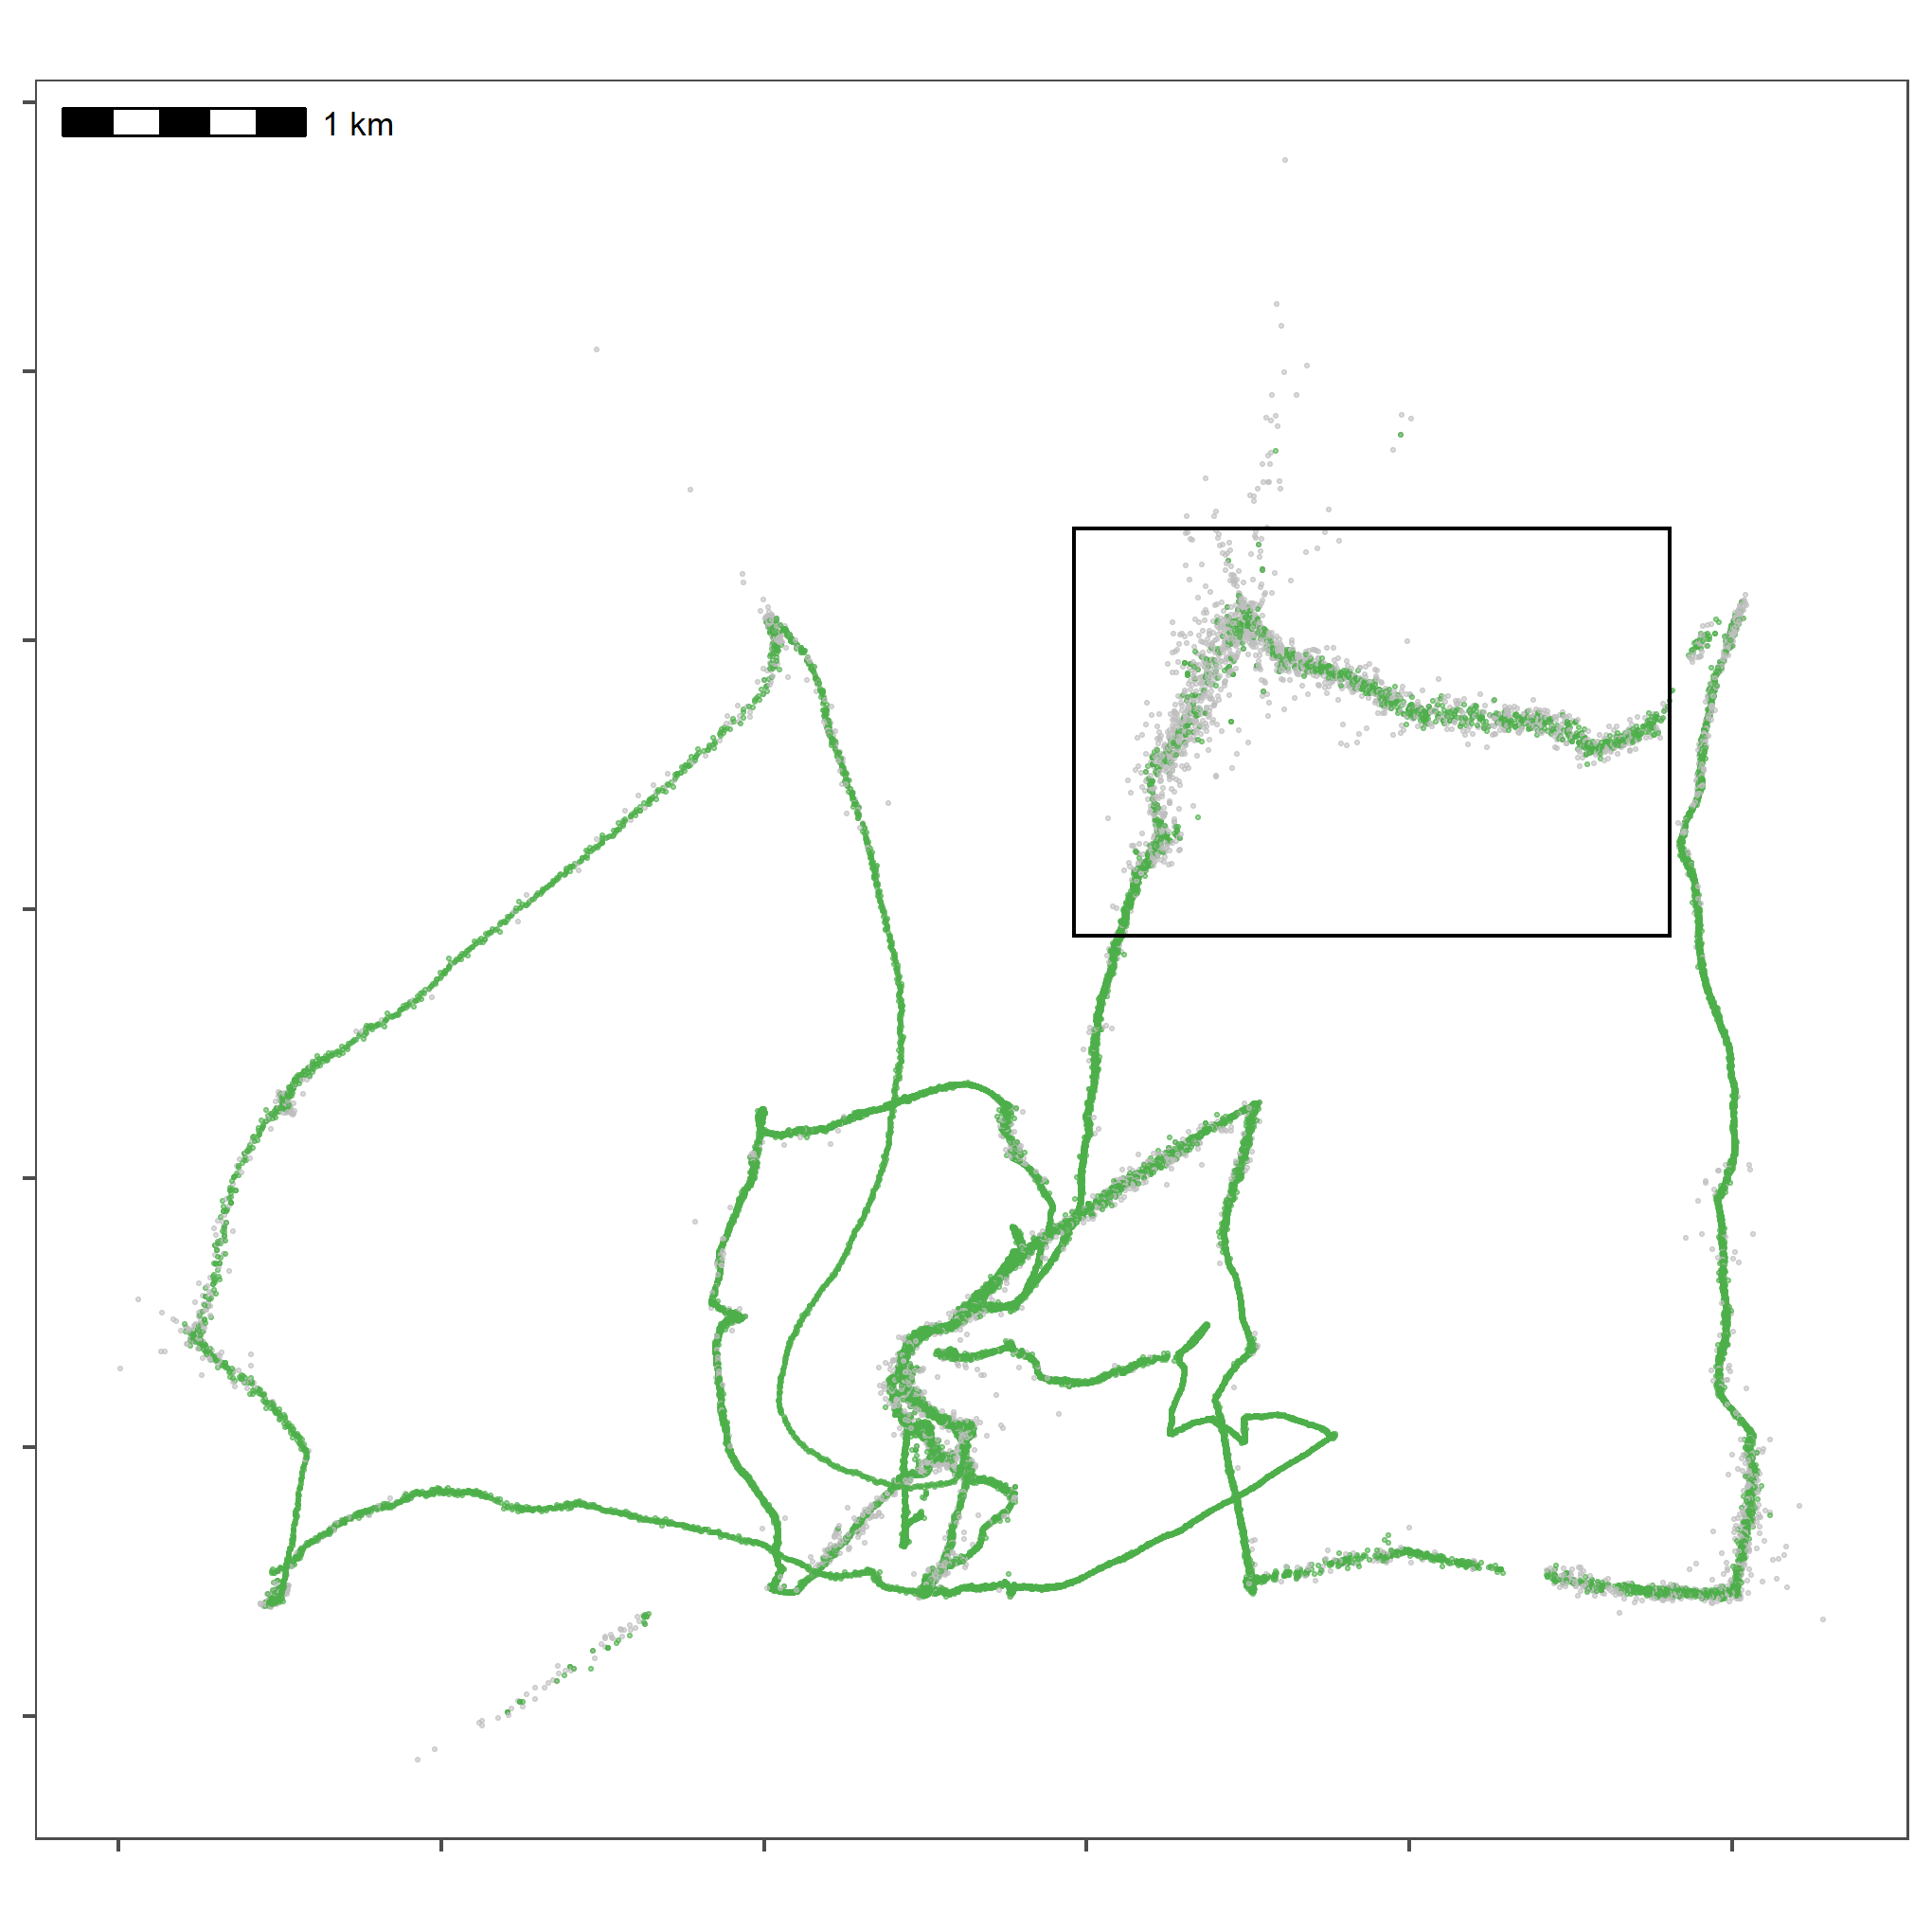
\includegraphics{figures/fig_speed_outlier.png}

\hypertarget{filter-on-speed}{%
\subsection{Filter on speed}\label{filter-on-speed}}

Here we use a speed threshold of 15 m/s, the fastest known boat speed.

\begin{Shaded}
\begin{Highlighting}[]
\CommentTok{\# make a copy}
\NormalTok{data\_unproc <{-}}\StringTok{ }\KeywordTok{copy}\NormalTok{(data)}

\CommentTok{\# remove speed outliers}
\NormalTok{data <{-}}\StringTok{ }\KeywordTok{atl\_filter\_covariates}\NormalTok{(}\DataTypeTok{data =}\NormalTok{ data,}
            \DataTypeTok{filters =} \KeywordTok{c}\NormalTok{(}\StringTok{"(speed\_in < 15 \& speed\_out < 15)"}\NormalTok{))}

\CommentTok{\# recalculate speed and angle}
\NormalTok{data[, }\StringTok{\textasciigrave{}}\DataTypeTok{:=}\StringTok{\textasciigrave{}}\NormalTok{ (}\DataTypeTok{speed\_in =} \KeywordTok{atl\_get\_speed}\NormalTok{(data, }
                                      \DataTypeTok{x =} \StringTok{"x"}\NormalTok{, }
                                      \DataTypeTok{y =} \StringTok{"y"}\NormalTok{, }
                                      \DataTypeTok{time =} \StringTok{"time"}\NormalTok{),}
             \DataTypeTok{speed\_out =} \KeywordTok{atl\_get\_speed}\NormalTok{(data, }\DataTypeTok{type =} \StringTok{"out"}\NormalTok{))]}

\CommentTok{\# add turning angle}
\NormalTok{data[, angle }\OperatorTok{:}\ErrorTok{=}\StringTok{ }\KeywordTok{atl\_turning\_angle}\NormalTok{(}\DataTypeTok{data =}\NormalTok{ data)]}
\end{Highlighting}
\end{Shaded}

\hypertarget{smoothing-the-trajectory}{%
\section{Smoothing the trajectory}\label{smoothing-the-trajectory}}

\begin{Shaded}
\begin{Highlighting}[]
\CommentTok{\# apply a 5 point median smooth, first make a copy}
\NormalTok{data\_unproc <{-}}\StringTok{ }\KeywordTok{copy}\NormalTok{(data)}

\CommentTok{\# now apply the smooth}
\NormalTok{data <{-}}\StringTok{ }\KeywordTok{atl\_median\_smooth}\NormalTok{(}\DataTypeTok{data =}\NormalTok{ data,}
                          \DataTypeTok{x =} \StringTok{"x"}\NormalTok{, }\DataTypeTok{y =} \StringTok{"y"}\NormalTok{, }\DataTypeTok{time =} \StringTok{"time"}\NormalTok{,}
                          \DataTypeTok{moving\_window =} \DecValTok{5}\NormalTok{)}
\end{Highlighting}
\end{Shaded}

\hypertarget{plot-pre-processing-steps}{%
\subsection{Plot pre-processing steps}\label{plot-pre-processing-steps}}

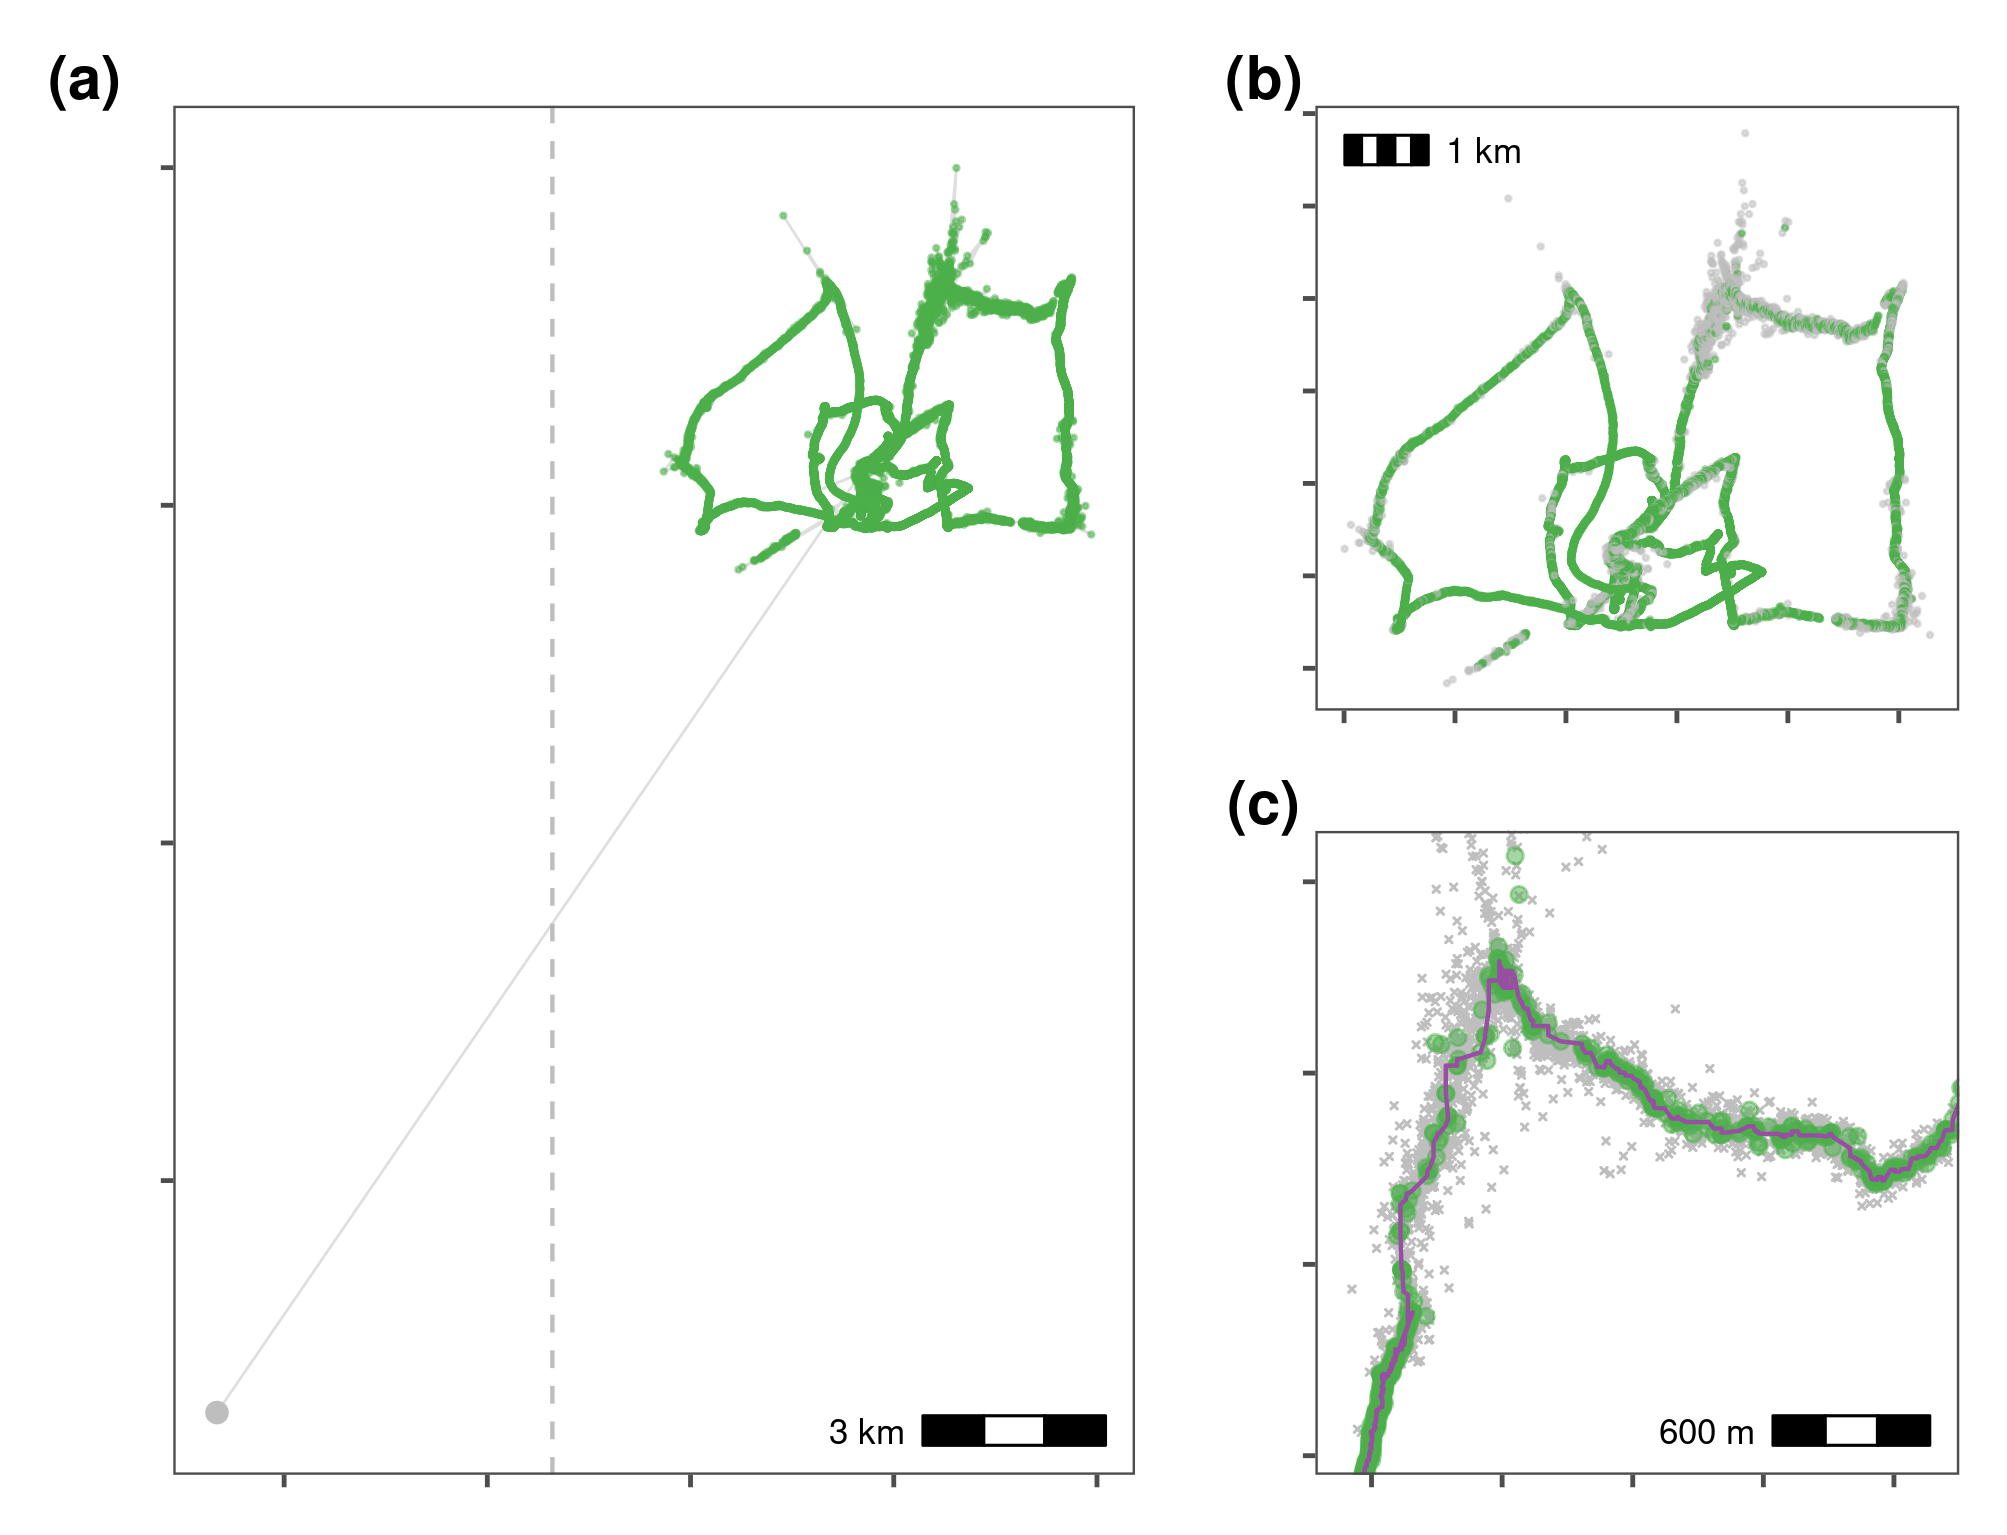
\includegraphics{figures/fig_walkthrough.png}

\hypertarget{making-residence-patches}{%
\section{Making residence patches}\label{making-residence-patches}}

\hypertarget{prepare-data}{%
\subsection{Prepare data}\label{prepare-data}}

An indicator of individual residence at or near a position can be useful when attempting to identify residence patches. Positions can be filtered on a metric such as residence time (see Bracis et al.~2018).

In this dataset, residence positions are marked in the \texttt{tID} column as beginning with \texttt{WP}. These can be extracted and converted into residence patches.

\begin{Shaded}
\begin{Highlighting}[]
\CommentTok{\# make a data copy}
\NormalTok{data\_unproc <{-}}\StringTok{ }\KeywordTok{copy}\NormalTok{(data)}
\end{Highlighting}
\end{Shaded}

\hypertarget{calculate-residence-time}{%
\subsection{Calculate residence time}\label{calculate-residence-time}}

Subset for boating segments: 2020-08-24 11:13:00 -- 2020-08-24 12:36:11.

\begin{Shaded}
\begin{Highlighting}[]
\CommentTok{\# load recurse}
\KeywordTok{library}\NormalTok{(recurse)}
\NormalTok{data\_recurse <{-}}\StringTok{ }\NormalTok{data\_unproc[, }\KeywordTok{list}\NormalTok{(x, y, time, TAG, UTCtime)]}

\CommentTok{\# thin the data}
\NormalTok{data\_recurse <{-}}\StringTok{ }\KeywordTok{atl\_thin\_data}\NormalTok{(}\DataTypeTok{data =}\NormalTok{ data\_recurse,}
                              \DataTypeTok{interval =} \DecValTok{30}\NormalTok{, }\DataTypeTok{id\_columns =} \StringTok{"TAG"}\NormalTok{,}
                              \DataTypeTok{method =} \StringTok{"resample"}\NormalTok{)}

\CommentTok{\# get 4 column data}
\NormalTok{data\_recurse <{-}}\StringTok{ }\NormalTok{data\_recurse[, }\KeywordTok{list}\NormalTok{(x, y, time, TAG)]}

\CommentTok{\# get recurse data for a 10m radius}
\NormalTok{recurse\_stats <{-}}\StringTok{ }\KeywordTok{getRecursions}\NormalTok{(data\_recurse,}
                               \DataTypeTok{radius =} \DecValTok{50}\NormalTok{, }\DataTypeTok{timeunits =} \StringTok{"mins"}\NormalTok{)}

\CommentTok{\# assign to recurse data}
\NormalTok{data\_recurse[, res\_time }\OperatorTok{:}\ErrorTok{=}\StringTok{ }\NormalTok{recurse\_stats}\OperatorTok{$}\NormalTok{residenceTime]}

\CommentTok{\# save recurse data}
\KeywordTok{fwrite}\NormalTok{(data\_recurse, }\DataTypeTok{file =} \StringTok{"data/data\_calib\_recurse.csv"}\NormalTok{)}
\end{Highlighting}
\end{Shaded}

Read in the data.

\begin{Shaded}
\begin{Highlighting}[]
\NormalTok{data\_recurse <{-}}\StringTok{ }\KeywordTok{fread}\NormalTok{(}\StringTok{"data/data\_calib\_recurse.csv"}\NormalTok{)}
\end{Highlighting}
\end{Shaded}

Subset waypoint data.

\begin{Shaded}
\begin{Highlighting}[]
\KeywordTok{library}\NormalTok{(stringi)}
\NormalTok{data\_res <{-}}\StringTok{ }\NormalTok{data\_unproc[}\KeywordTok{stri\_detect}\NormalTok{(tID, }\DataTypeTok{regex =} \StringTok{"(WP)"}\NormalTok{)]}
\end{Highlighting}
\end{Shaded}

\hypertarget{plot-residence-time}{%
\subsection{Plot residence time}\label{plot-residence-time}}

\hypertarget{run-residence-patch-method}{%
\subsection{Run residence patch method}\label{run-residence-patch-method}}

\begin{Shaded}
\begin{Highlighting}[]
\CommentTok{\# assign id as tag}
\NormalTok{data\_recurse[, id }\OperatorTok{:}\ErrorTok{=}\StringTok{ }\KeywordTok{as.character}\NormalTok{(TAG)]}

\CommentTok{\# subset on 5 minute residence time}
\NormalTok{data\_recurse\_subset <{-}}\StringTok{ }\NormalTok{data\_recurse[res\_time }\OperatorTok{>=}\StringTok{ }\DecValTok{5}\NormalTok{, ]}

\CommentTok{\# on known residence points}
\NormalTok{patch\_res\_known <{-}}\StringTok{ }\KeywordTok{atl\_res\_patch}\NormalTok{(data\_recurse\_subset, }
                                \DataTypeTok{buffer\_radius =} \DecValTok{10}\NormalTok{,}
                                \DataTypeTok{lim\_spat\_indep =} \DecValTok{100}\NormalTok{,}
                                \DataTypeTok{lim\_time\_indep =} \DecValTok{5}\NormalTok{,}
                                \DataTypeTok{min\_fixes =} \DecValTok{3}\NormalTok{)}
\end{Highlighting}
\end{Shaded}

\hypertarget{get-spatial-and-summary-objects}{%
\subsection{Get spatial and summary objects}\label{get-spatial-and-summary-objects}}

\begin{Shaded}
\begin{Highlighting}[]
\CommentTok{\# for the known and unkniwn patches}
\NormalTok{patch\_sf\_data <{-}}\StringTok{ }\KeywordTok{atl\_patch\_summary}\NormalTok{(patch\_res\_known, }\DataTypeTok{which\_data =} \StringTok{"spatial"}\NormalTok{,}
                                   \DataTypeTok{buffer\_radius =} \DecValTok{20}\NormalTok{)}

\CommentTok{\# assign crs}
\NormalTok{sf}\OperatorTok{::}\KeywordTok{st\_crs}\NormalTok{(patch\_sf\_data) <{-}}\StringTok{ }\DecValTok{32631}

\CommentTok{\# get summary data}
\NormalTok{patch\_summary\_data <{-}}\StringTok{ }\KeywordTok{atl\_patch\_summary}\NormalTok{(patch\_res\_known, }\DataTypeTok{which\_data =} \StringTok{"summary"}\NormalTok{)}
\end{Highlighting}
\end{Shaded}

\hypertarget{get-waypoint-centroids}{%
\subsection{Get waypoint centroids}\label{get-waypoint-centroids}}

\begin{Shaded}
\begin{Highlighting}[]
\CommentTok{\# get centroid}
\NormalTok{data\_res\_summary <{-}}\StringTok{ }\NormalTok{data\_res[, }\KeywordTok{list}\NormalTok{(}\DataTypeTok{x\_median =} \KeywordTok{median}\NormalTok{(x),}
                                    \DataTypeTok{y\_median =} \KeywordTok{median}\NormalTok{(y),}
                                    \DataTypeTok{t\_median =} \KeywordTok{median}\NormalTok{(time)),}
\NormalTok{                             by =}\StringTok{ "tID"}\NormalTok{]}

\CommentTok{\# now get times 10 mins before and after}
\NormalTok{data\_res\_summary[, }\StringTok{\textasciigrave{}}\DataTypeTok{:=}\StringTok{\textasciigrave{}}\NormalTok{(}\DataTypeTok{t\_min =}\NormalTok{ t\_median }\OperatorTok{{-}}\StringTok{ }\NormalTok{(}\DecValTok{10} \OperatorTok{*}\StringTok{ }\DecValTok{60}\NormalTok{),}
                        \DataTypeTok{t\_max =}\NormalTok{ t\_median }\OperatorTok{+}\StringTok{ }\NormalTok{(}\DecValTok{10} \OperatorTok{*}\StringTok{ }\DecValTok{60}\NormalTok{))]}

\CommentTok{\# make a list of positions 10min before and after}
\NormalTok{wp\_data <{-}}\StringTok{ }\KeywordTok{mapply}\NormalTok{(}\ControlFlowTok{function}\NormalTok{(l, u, mx, my) \{}
\NormalTok{  tmp\_data <{-}}\StringTok{ }\NormalTok{data\_unproc[}\KeywordTok{inrange}\NormalTok{(time, l, u)]}
\NormalTok{  tmp\_data[, distance }\OperatorTok{:}\ErrorTok{=}\StringTok{ }\KeywordTok{sqrt}\NormalTok{((mx }\OperatorTok{{-}}\StringTok{ }\NormalTok{x)}\OperatorTok{\^{}}\DecValTok{2} \OperatorTok{+}\StringTok{ }\NormalTok{(my }\OperatorTok{{-}}\StringTok{ }\NormalTok{y)}\OperatorTok{\^{}}\DecValTok{2}\NormalTok{)]}
  \CommentTok{\# keep within 50}
\NormalTok{  tmp\_data <{-}}\StringTok{ }\NormalTok{tmp\_data[distance }\OperatorTok{<=}\StringTok{ }\DecValTok{50}\NormalTok{, ]}
  \CommentTok{\# get duration}
  \KeywordTok{return}\NormalTok{(}\KeywordTok{diff}\NormalTok{(}\KeywordTok{range}\NormalTok{(tmp\_data}\OperatorTok{$}\NormalTok{time)))}
\NormalTok{\}, data\_res\_summary}\OperatorTok{$}\NormalTok{t\_min, data\_res\_summary}\OperatorTok{$}\NormalTok{t\_max,}
\NormalTok{   data\_res\_summary}\OperatorTok{$}\NormalTok{x\_median, data\_res\_summary}\OperatorTok{$}\NormalTok{y\_median,}
\DataTypeTok{SIMPLIFY =} \OtherTok{FALSE}\NormalTok{)}
\end{Highlighting}
\end{Shaded}

\hypertarget{read-griend}{%
\subsection{Read Griend}\label{read-griend}}

\begin{Shaded}
\begin{Highlighting}[]
\CommentTok{\# read griend}
\NormalTok{griend <{-}}\StringTok{ }\NormalTok{sf}\OperatorTok{::}\KeywordTok{st\_read}\NormalTok{(}\StringTok{"data/griend\_polygon/griend\_polygon.shp"}\NormalTok{)}
\end{Highlighting}
\end{Shaded}

We prepare a plot of the residence patches.

\hypertarget{compare-patch-metrics}{%
\section{Compare patch metrics}\label{compare-patch-metrics}}

\hypertarget{compare-known-patches}{%
\subsection{Compare known patches}\label{compare-known-patches}}

\begin{Shaded}
\begin{Highlighting}[]
\CommentTok{\# get known patch summary}
\NormalTok{data\_res <{-}}\StringTok{ }\NormalTok{data\_unproc[stringi}\OperatorTok{::}\KeywordTok{stri\_detect}\NormalTok{(tID, }\DataTypeTok{regex =} \StringTok{"(WP)"}\NormalTok{), ]}

\CommentTok{\# get waypoint summary}
\NormalTok{patch\_summary\_real <{-}}\StringTok{ }\NormalTok{data\_res[, }\KeywordTok{list}\NormalTok{(}\DataTypeTok{nfixes\_real =}\NormalTok{ .N,}
                                      \DataTypeTok{x\_median =} \KeywordTok{round}\NormalTok{(}\KeywordTok{median}\NormalTok{(x), }\DataTypeTok{digits =} \DecValTok{{-}2}\NormalTok{),}
                                      \DataTypeTok{y\_median =} \KeywordTok{round}\NormalTok{(}\KeywordTok{median}\NormalTok{(y), }\DataTypeTok{digits =} \DecValTok{{-}2}\NormalTok{)), }
\NormalTok{                               by =}\StringTok{ "tID"}\NormalTok{]}

\CommentTok{\# add real duration}
\NormalTok{patch\_summary\_real[, duration\_real }\OperatorTok{:}\ErrorTok{=}\StringTok{ }\KeywordTok{unlist}\NormalTok{(wp\_data)]}
\CommentTok{\# round median coordinate for inferred patches}
\NormalTok{patch\_summary\_inferred <{-}}\StringTok{ }
\StringTok{  }\NormalTok{patch\_summary\_data[, }
                     \KeywordTok{c}\NormalTok{(}\StringTok{"x\_median"}\NormalTok{, }\StringTok{"y\_median"}\NormalTok{, }
                       \StringTok{"nfixes"}\NormalTok{, }\StringTok{"duration"}\NormalTok{, }\StringTok{"patch"}\NormalTok{)}
\NormalTok{                     ][, }\StringTok{\textasciigrave{}}\DataTypeTok{:=}\StringTok{\textasciigrave{}}\NormalTok{(}\DataTypeTok{x\_median =} \KeywordTok{round}\NormalTok{(x\_median, }\DataTypeTok{digits =} \DecValTok{{-}2}\NormalTok{),}
                              \DataTypeTok{y\_median =} \KeywordTok{round}\NormalTok{(y\_median, }\DataTypeTok{digits =} \DecValTok{{-}2}\NormalTok{))]}

\CommentTok{\# join with respatch summary}
\NormalTok{patch\_summary\_compare <{-}}\StringTok{ }
\StringTok{  }\KeywordTok{merge}\NormalTok{(patch\_summary\_real,}
\NormalTok{        patch\_summary\_inferred, }
        \DataTypeTok{on =} \KeywordTok{c}\NormalTok{(}\StringTok{"x\_median"}\NormalTok{, }\StringTok{"y\_median"}\NormalTok{),}
        \DataTypeTok{all.x =} \OtherTok{TRUE}\NormalTok{, }\DataTypeTok{all.y =} \OtherTok{TRUE}\NormalTok{)}

\NormalTok{patch\_summary\_compare[}\OperatorTok{!}\KeywordTok{is.na}\NormalTok{(tID)]}

\CommentTok{\# drop nas}
\NormalTok{patch\_summary\_compare <{-}}\StringTok{ }\KeywordTok{na.omit}\NormalTok{(patch\_summary\_compare)}

\CommentTok{\# drop patch around WP080}
\NormalTok{patch\_summary\_compare <{-}}\StringTok{ }\NormalTok{patch\_summary\_compare[tID }\OperatorTok{!=}\StringTok{ "WP080"}\NormalTok{, ]}
\end{Highlighting}
\end{Shaded}

12 patches are identified where there are no waypoints, while 2 waypoints are not identified as patches. These waypoints consisted of 6 and 15 (WP098 and WP092) positions respectively, and were lost when the data were aggregated to 30 second intervals.

\hypertarget{plot-durations-comparisons}{%
\subsection{Plot durations comparisons}\label{plot-durations-comparisons}}

\begin{Shaded}
\begin{Highlighting}[]
\CommentTok{\# get linear model}
\NormalTok{model\_duration <{-}}\StringTok{ }\KeywordTok{lm}\NormalTok{(duration\_real }\OperatorTok{\textasciitilde{}}\StringTok{ }\NormalTok{duration,}
                     \DataTypeTok{data =}\NormalTok{ patch\_summary\_compare)}

\CommentTok{\# get R2}
\KeywordTok{summary}\NormalTok{(model\_duration)}
\end{Highlighting}
\end{Shaded}

\hypertarget{join-patch-map-and-duration-comparison-figure}{%
\subsection{Join patch map and duration comparison figure}\label{join-patch-map-and-duration-comparison-figure}}

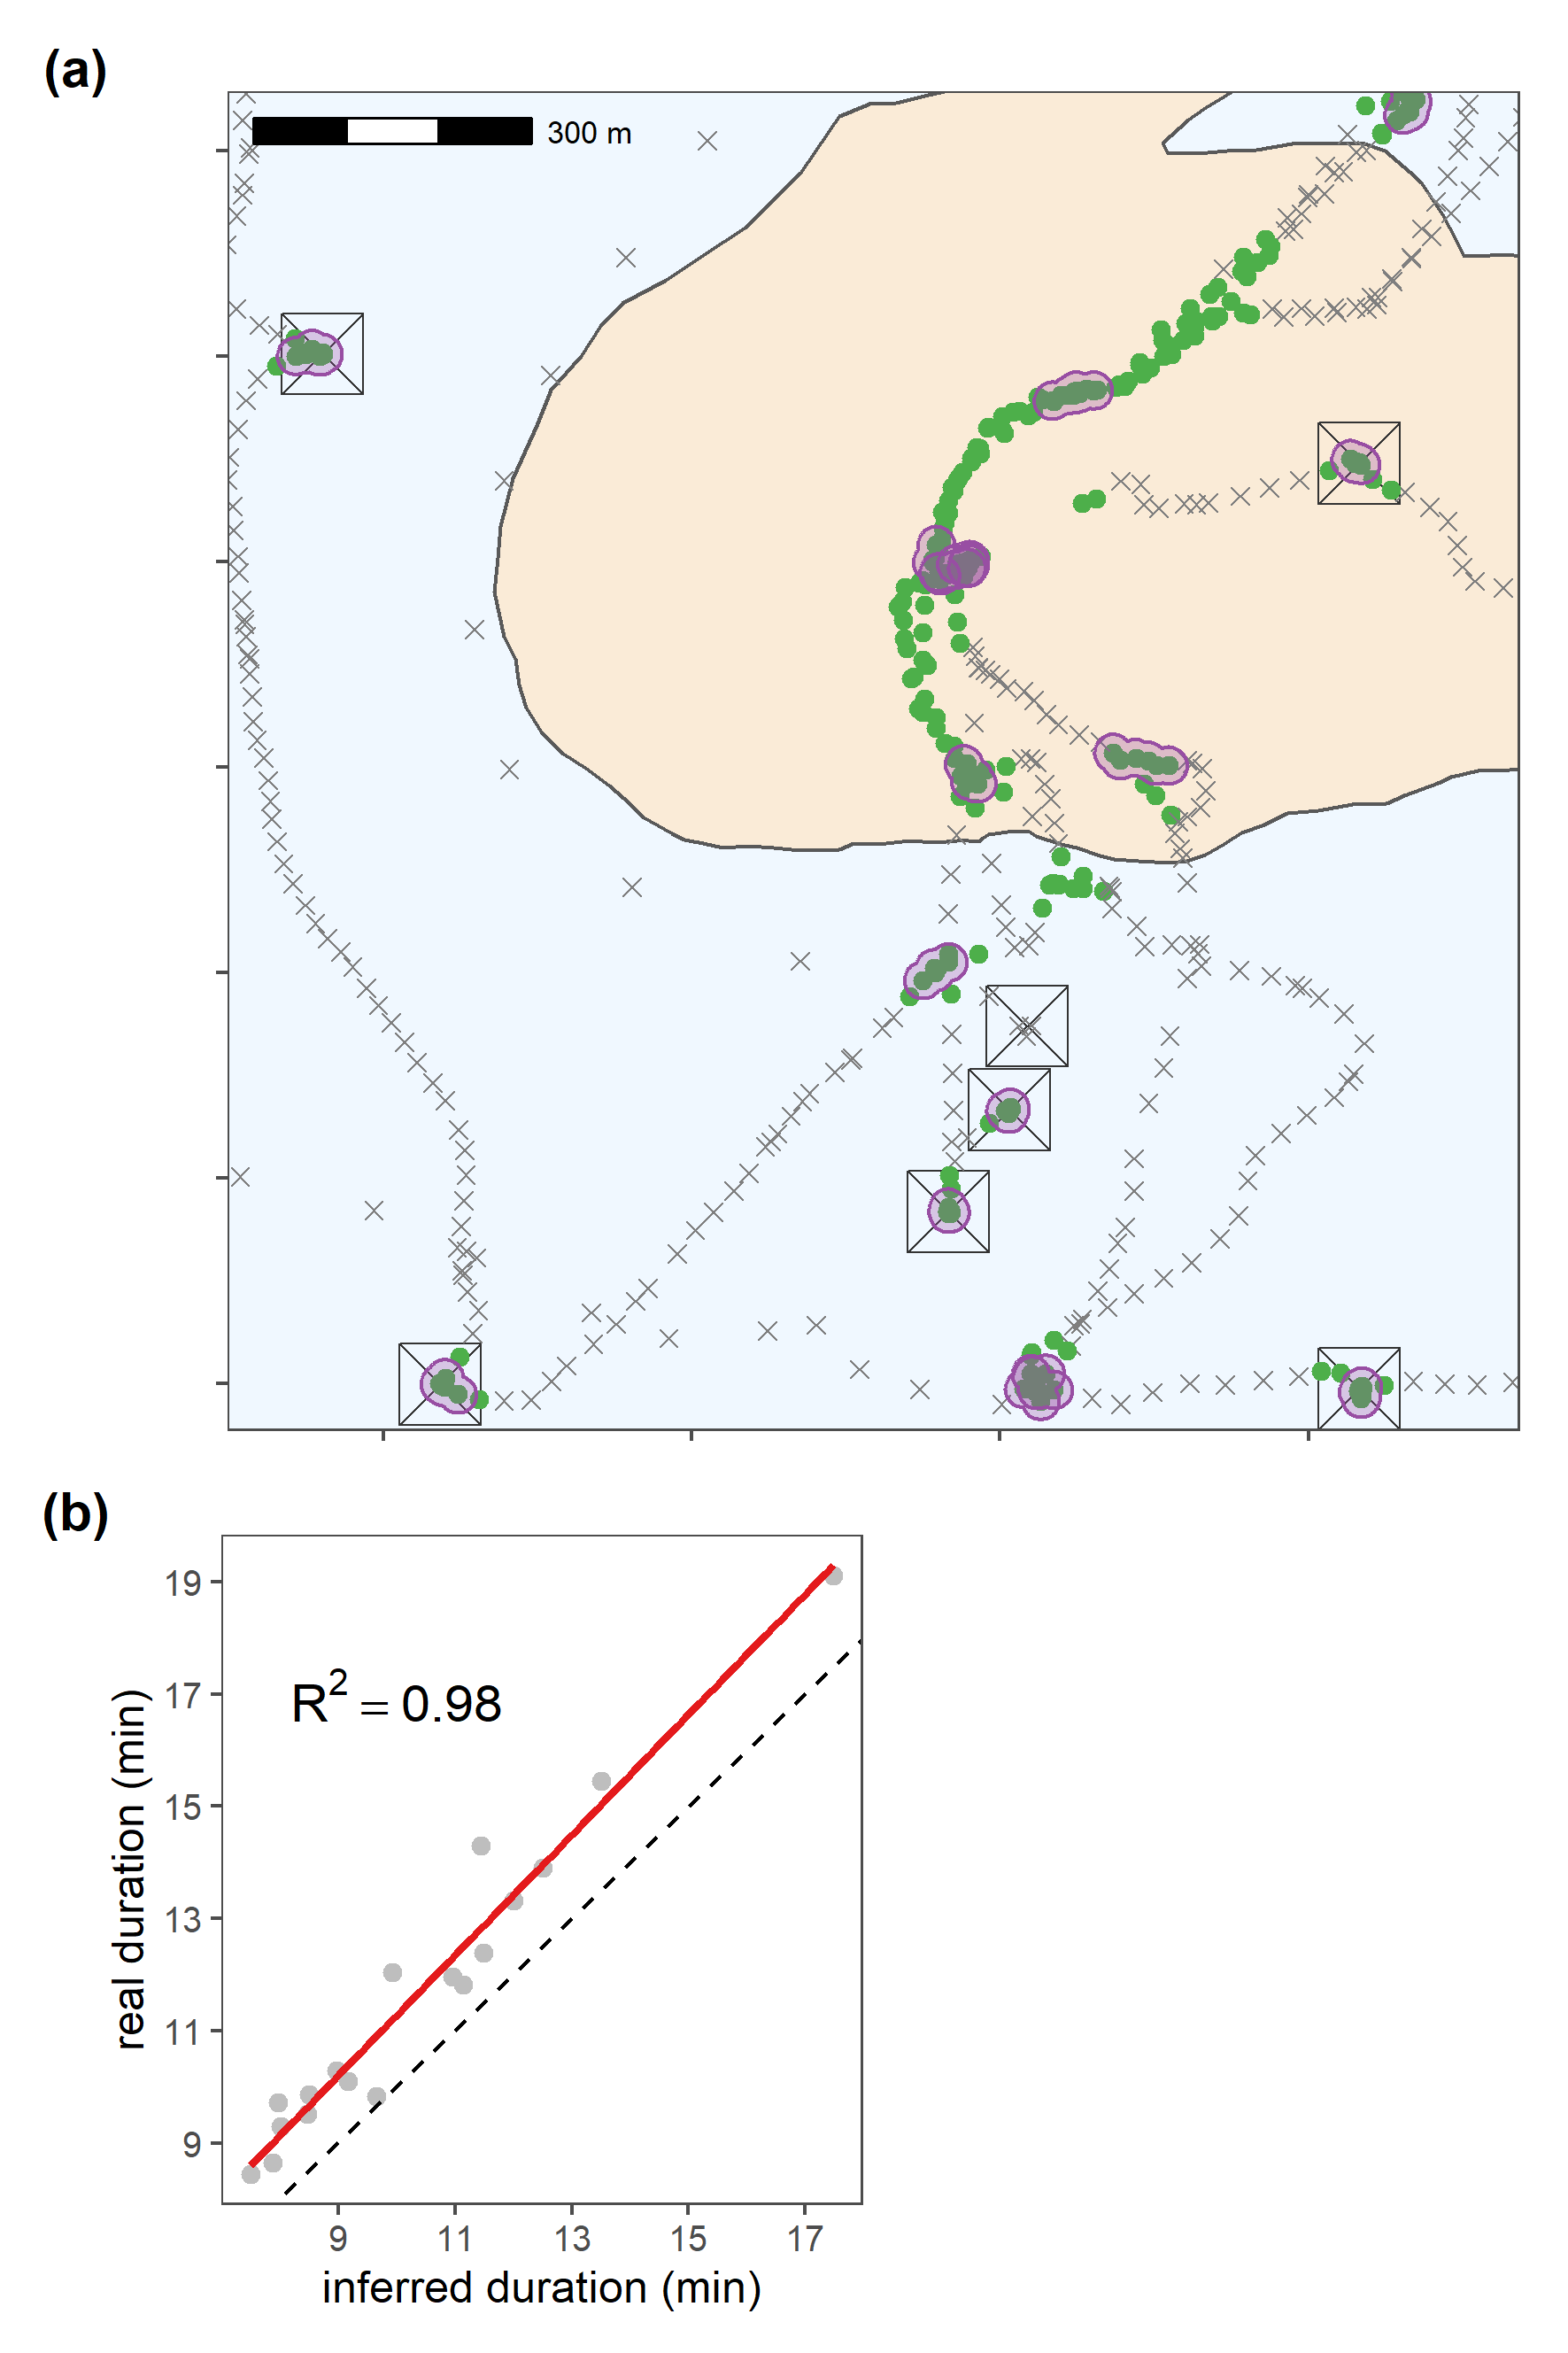
\includegraphics{figures/fig_calib_residence_patch.png}

\hypertarget{processing-egyptian-fruit-bat-tracks}{%
\chapter{Processing Egyptian fruit bat tracks}\label{processing-egyptian-fruit-bat-tracks}}

We show the pre-processing pipeline at work on the tracks of three Egyptian fruit bats (\emph{Rousettus aegyptiacus}), and construct residence patches.

\hypertarget{prepare-libraries}{%
\section{Prepare libraries}\label{prepare-libraries}}

\begin{Shaded}
\begin{Highlighting}[]
\CommentTok{\# load libs}
\KeywordTok{library}\NormalTok{(data.table)}
\KeywordTok{library}\NormalTok{(RSQLite)}
\KeywordTok{library}\NormalTok{(atlastools)}
\KeywordTok{library}\NormalTok{(ggplot2)}
\KeywordTok{library}\NormalTok{(patchwork)}

\CommentTok{\# prepare a palette}
\NormalTok{pal <{-}}\StringTok{ }\NormalTok{RColorBrewer}\OperatorTok{::}\KeywordTok{brewer.pal}\NormalTok{(}\DecValTok{4}\NormalTok{, }\StringTok{"Set1"}\NormalTok{)}
\end{Highlighting}
\end{Shaded}

\hypertarget{read-bat-data}{%
\section{Read bat data}\label{read-bat-data}}

Read the bat data and convert to a csv file.

\begin{Shaded}
\begin{Highlighting}[]
\CommentTok{\# prepare the connection}
\NormalTok{con <{-}}\StringTok{ }\KeywordTok{dbConnect}\NormalTok{(}\DataTypeTok{drv =} \KeywordTok{SQLite}\NormalTok{(), }\DataTypeTok{dbname =} \StringTok{"data/Three\_example\_bats.sql"}\NormalTok{)}

\CommentTok{\# list the tables}
\NormalTok{table\_name <{-}}\StringTok{ }\KeywordTok{dbListTables}\NormalTok{(con)}

\CommentTok{\# prepare to query all tables}
\NormalTok{query <{-}}\StringTok{ }\KeywordTok{sprintf}\NormalTok{(}\StringTok{\textquotesingle{}select * from }\CharTok{\textbackslash{}"}\StringTok{\%s}\CharTok{\textbackslash{}"}\StringTok{\textquotesingle{}}\NormalTok{, table\_name)}

\CommentTok{\# query the database}
\NormalTok{data <{-}}\StringTok{ }\KeywordTok{dbGetQuery}\NormalTok{(}\DataTypeTok{conn =}\NormalTok{ con, }\DataTypeTok{statement =}\NormalTok{ query)}

\CommentTok{\# disconnect from database}
\KeywordTok{dbDisconnect}\NormalTok{(con)}
\end{Highlighting}
\end{Shaded}

Convert data to csv.

\begin{Shaded}
\begin{Highlighting}[]
\CommentTok{\# convert data to datatable}
\KeywordTok{setDT}\NormalTok{(data)}

\CommentTok{\# write data for QGIS}
\KeywordTok{fwrite}\NormalTok{(data, }\DataTypeTok{file =} \StringTok{"data/bat\_data.csv"}\NormalTok{)}
\end{Highlighting}
\end{Shaded}

\hypertarget{sanity-check-plot-bat-data}{%
\section{Sanity check: Plot bat data}\label{sanity-check-plot-bat-data}}

Save the raw data plot.

Show the plot.

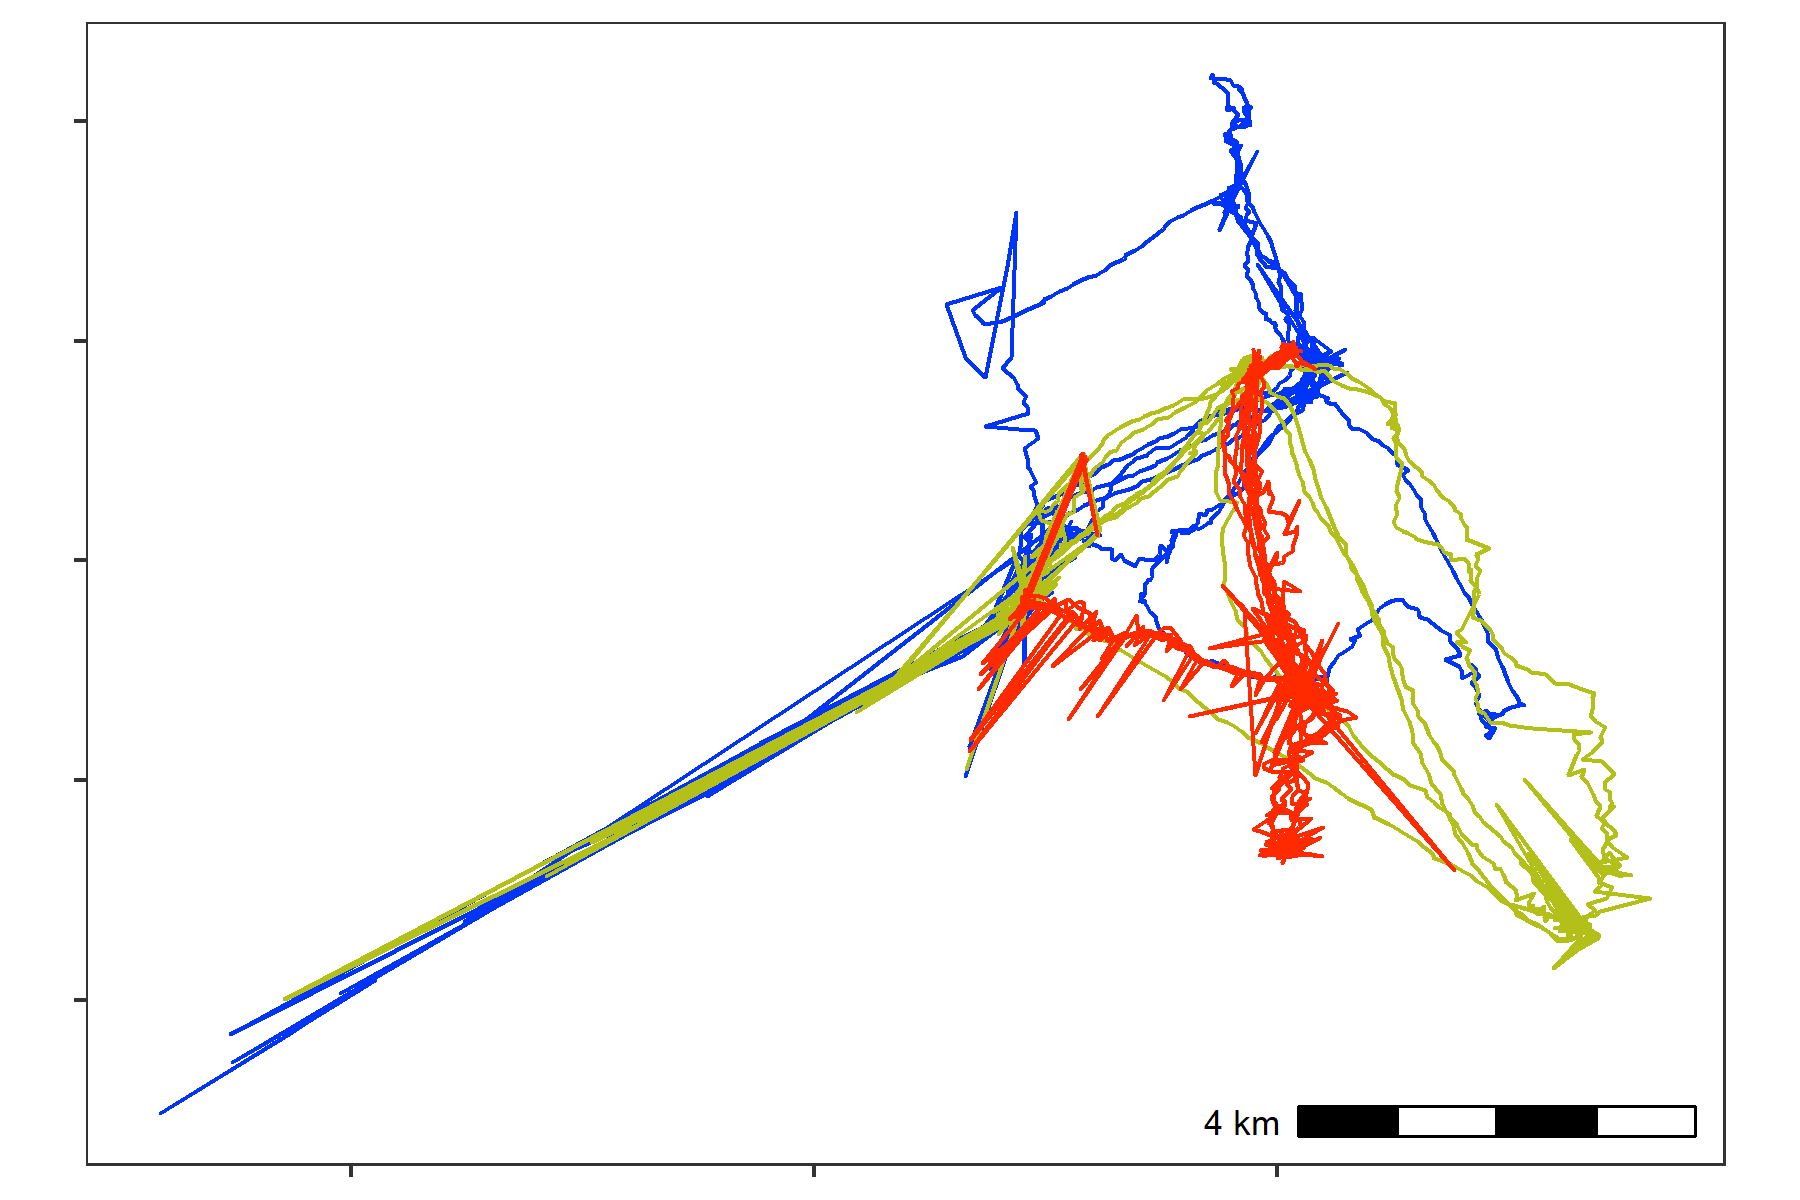
\includegraphics{figures/fig_bat_raw.png}

\hypertarget{prepare-data-for-filtering}{%
\section{Prepare data for filtering}\label{prepare-data-for-filtering}}

\hypertarget{prepare-data-per-individual}{%
\subsection{Prepare data per individual}\label{prepare-data-per-individual}}

\begin{Shaded}
\begin{Highlighting}[]
\CommentTok{\# split bat data by tag}
\CommentTok{\# first make a copy using the data.table function copy}
\CommentTok{\# this prevents the orignal data from being modified by atlastools}
\CommentTok{\# functions which DO MODIFY BY REFERENCE!}
\NormalTok{data\_split <{-}}\StringTok{ }\KeywordTok{copy}\NormalTok{(data)}

\CommentTok{\# now split}
\NormalTok{data\_split <{-}}\StringTok{ }\KeywordTok{split}\NormalTok{(data\_split, data}\OperatorTok{$}\NormalTok{TAG)}
\end{Highlighting}
\end{Shaded}

\hypertarget{filter-by-covariates}{%
\section{Filter by covariates}\label{filter-by-covariates}}

No natural bounds suggest themselves, and we proceed to filter by covariates, since point outliers are obviously visible.

We use filter out positions with \texttt{SD\ \textgreater{}\ 20} and positions calculated using only 3 base stations.

We use the function \texttt{atl\_filter\_covariates}.

\begin{Shaded}
\begin{Highlighting}[]
\CommentTok{\# get SD.}
\CommentTok{\# since the data are data.tables, no assignment is necessary}
\KeywordTok{invisible}\NormalTok{(}
  \KeywordTok{lapply}\NormalTok{(data\_split, }\ControlFlowTok{function}\NormalTok{(dt) \{}
\NormalTok{    dt[, SD }\OperatorTok{:}\ErrorTok{=}\StringTok{ }\KeywordTok{sqrt}\NormalTok{(VARX }\OperatorTok{+}\StringTok{ }\NormalTok{VARY }\OperatorTok{+}\StringTok{ }\NormalTok{(}\DecValTok{2} \OperatorTok{*}\StringTok{ }\NormalTok{COVXY))]}
\NormalTok{  \})}
\NormalTok{)}

\CommentTok{\# filter for SD <= 20}
\CommentTok{\# here, reassignment is necessary as rows are being removed}
\CommentTok{\# the atl\_filter\_covariates function could have been used here}
\NormalTok{data\_split <{-}}\StringTok{ }\KeywordTok{lapply}\NormalTok{(data\_split, }\ControlFlowTok{function}\NormalTok{(dt) \{}
\NormalTok{  dt <{-}}\StringTok{ }\KeywordTok{atl\_filter\_covariates}\NormalTok{(}
    \DataTypeTok{data =}\NormalTok{ dt,}
    \DataTypeTok{filters =} \KeywordTok{c}\NormalTok{(}\StringTok{"SD <= 20"}\NormalTok{,}
                \StringTok{"NBS > 3"}\NormalTok{)}
\NormalTok{  )}
\NormalTok{\})}

\CommentTok{\# check whether the filter has worked}
\KeywordTok{invisible}\NormalTok{(}
  \KeywordTok{lapply}\NormalTok{(data\_split, }\ControlFlowTok{function}\NormalTok{(dt) \{}
\NormalTok{    assertthat}\OperatorTok{::}\KeywordTok{assert\_that}\NormalTok{(}\KeywordTok{min}\NormalTok{(dt}\OperatorTok{$}\NormalTok{SD) }\OperatorTok{<=}\StringTok{ }\DecValTok{20}\NormalTok{,}
                            \DataTypeTok{msg =} \StringTok{"some SDs above 20 remain"}\NormalTok{)}
\NormalTok{    assertthat}\OperatorTok{::}\KeywordTok{assert\_that}\NormalTok{(}\KeywordTok{min}\NormalTok{(dt}\OperatorTok{$}\NormalTok{NBS) }\OperatorTok{>}\StringTok{ }\DecValTok{3}\NormalTok{,}
                            \DataTypeTok{msg =} \StringTok{"some NBS below 3 remain"}\NormalTok{)}
\NormalTok{  \})}
\NormalTok{)}
\end{Highlighting}
\end{Shaded}

\hypertarget{sanity-check-plot-filtered-data}{%
\subsection{Sanity check: Plot filtered data}\label{sanity-check-plot-filtered-data}}

\begin{Shaded}
\begin{Highlighting}[]
\CommentTok{\# bind all individuals together}
\NormalTok{data\_split <{-}}\StringTok{ }\KeywordTok{rbindlist}\NormalTok{(data\_split)}
\end{Highlighting}
\end{Shaded}

Save the filtered data plot.

Show the plot.

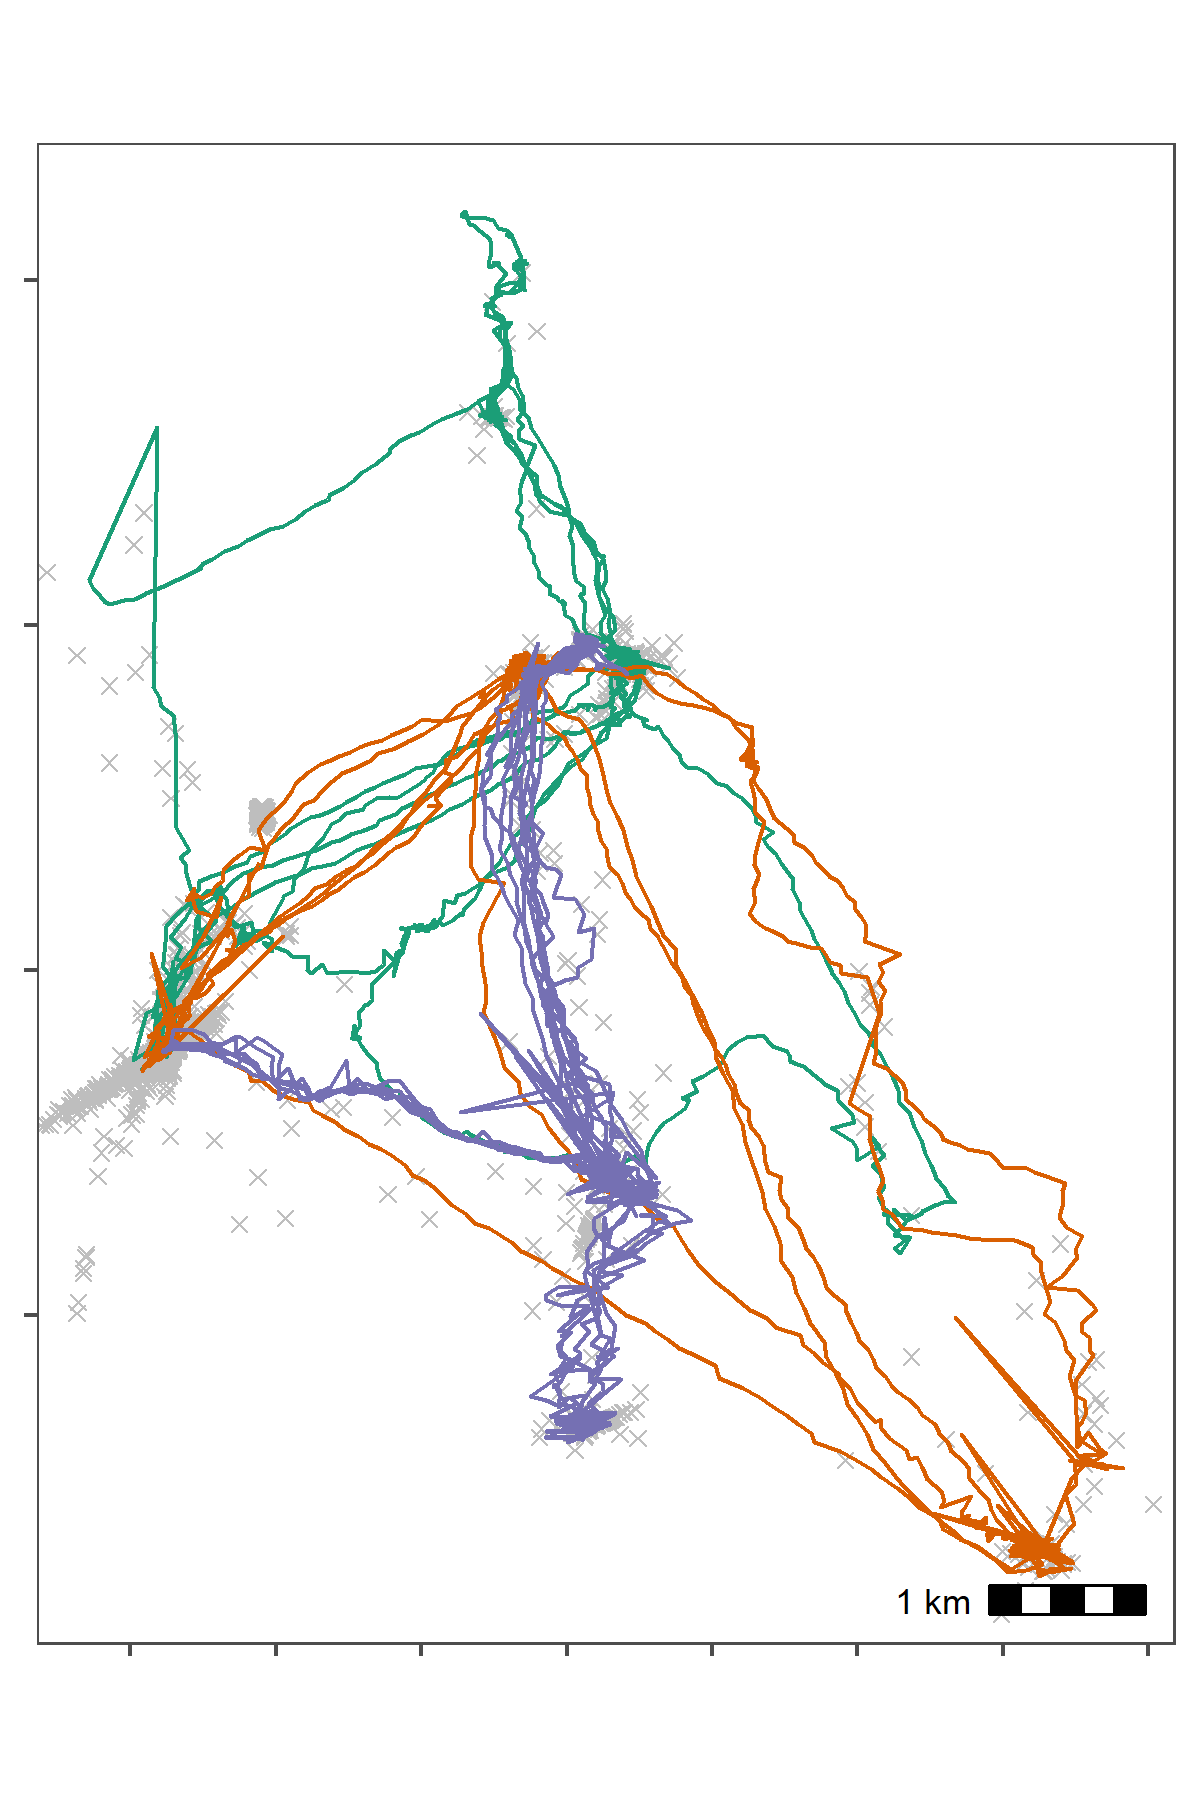
\includegraphics{figures/fig_bat_filter_cov.png}

\hypertarget{filter-by-speed}{%
\section{Filter by speed}\label{filter-by-speed}}

Some point outliers remain, and should be removed using a speed filter.

First we calculate speeds.

\begin{Shaded}
\begin{Highlighting}[]
\CommentTok{\# calculate speed on split data once more}
\NormalTok{data\_split <{-}}\StringTok{ }\KeywordTok{split}\NormalTok{(data\_split, data\_split}\OperatorTok{$}\NormalTok{TAG)}

\CommentTok{\# get speeds as with SD, no reassignment required for columns}
\KeywordTok{invisible}\NormalTok{(}
  \KeywordTok{lapply}\NormalTok{(data\_split, }\ControlFlowTok{function}\NormalTok{(dt) \{}
    
    \CommentTok{\# first process time to seconds}
    \CommentTok{\# assign to a new column}
\NormalTok{    dt[, time }\OperatorTok{:}\ErrorTok{=}\StringTok{ }\KeywordTok{floor}\NormalTok{(TIME }\OperatorTok{/}\StringTok{ }\DecValTok{1000}\NormalTok{)]}
    
\NormalTok{    dt[, }\StringTok{\textasciigrave{}}\DataTypeTok{:=}\StringTok{\textasciigrave{}}\NormalTok{(}\DataTypeTok{speed\_in =} \KeywordTok{atl\_get\_speed}\NormalTok{(dt, }
                                       \DataTypeTok{x =} \StringTok{"X"}\NormalTok{, }\DataTypeTok{y =} \StringTok{"Y"}\NormalTok{, }
                                       \DataTypeTok{time =} \StringTok{"time"}\NormalTok{,}
                                       \DataTypeTok{type =} \StringTok{"in"}\NormalTok{),}
              \DataTypeTok{speed\_out =} \KeywordTok{atl\_get\_speed}\NormalTok{(dt, }
                                       \DataTypeTok{x =} \StringTok{"X"}\NormalTok{, }\DataTypeTok{y =} \StringTok{"Y"}\NormalTok{, }
                                       \DataTypeTok{time =} \StringTok{"time"}\NormalTok{,}
                                       \DataTypeTok{type =} \StringTok{"out"}\NormalTok{))]}
\NormalTok{  \})}
\NormalTok{)}
\end{Highlighting}
\end{Shaded}

Now filter for speeds \textgreater{} 20 m/s (around 70 km/h).

\begin{Shaded}
\begin{Highlighting}[]
\CommentTok{\# filter speeds}
\CommentTok{\# reassignment is required here}
\NormalTok{data\_split <{-}}\StringTok{ }\KeywordTok{lapply}\NormalTok{(data\_split, }\ControlFlowTok{function}\NormalTok{(dt) \{}
\NormalTok{  dt <{-}}\StringTok{ }\KeywordTok{na.omit}\NormalTok{(dt, }\DataTypeTok{cols =} \KeywordTok{c}\NormalTok{(}\StringTok{"speed\_in"}\NormalTok{, }\StringTok{"speed\_out"}\NormalTok{))}
  
\NormalTok{  dt <{-}}\StringTok{ }\KeywordTok{atl\_filter\_covariates}\NormalTok{(}\DataTypeTok{data =}\NormalTok{ dt,}
                              \DataTypeTok{filters =} \KeywordTok{c}\NormalTok{(}\StringTok{"speed\_in <= 20"}\NormalTok{,}
                                          \StringTok{"speed\_out <= 20"}\NormalTok{))}
\NormalTok{\})}
\end{Highlighting}
\end{Shaded}

\hypertarget{sanity-check-plot-speed-filtered-data}{%
\subsection{Sanity check: Plot speed filtered data}\label{sanity-check-plot-speed-filtered-data}}

\begin{Shaded}
\begin{Highlighting}[]
\CommentTok{\# bind all individuals together}
\NormalTok{data\_split <{-}}\StringTok{ }\KeywordTok{rbindlist}\NormalTok{(data\_split)}
\end{Highlighting}
\end{Shaded}

Save the speed filtered data plot.

Show the plot.

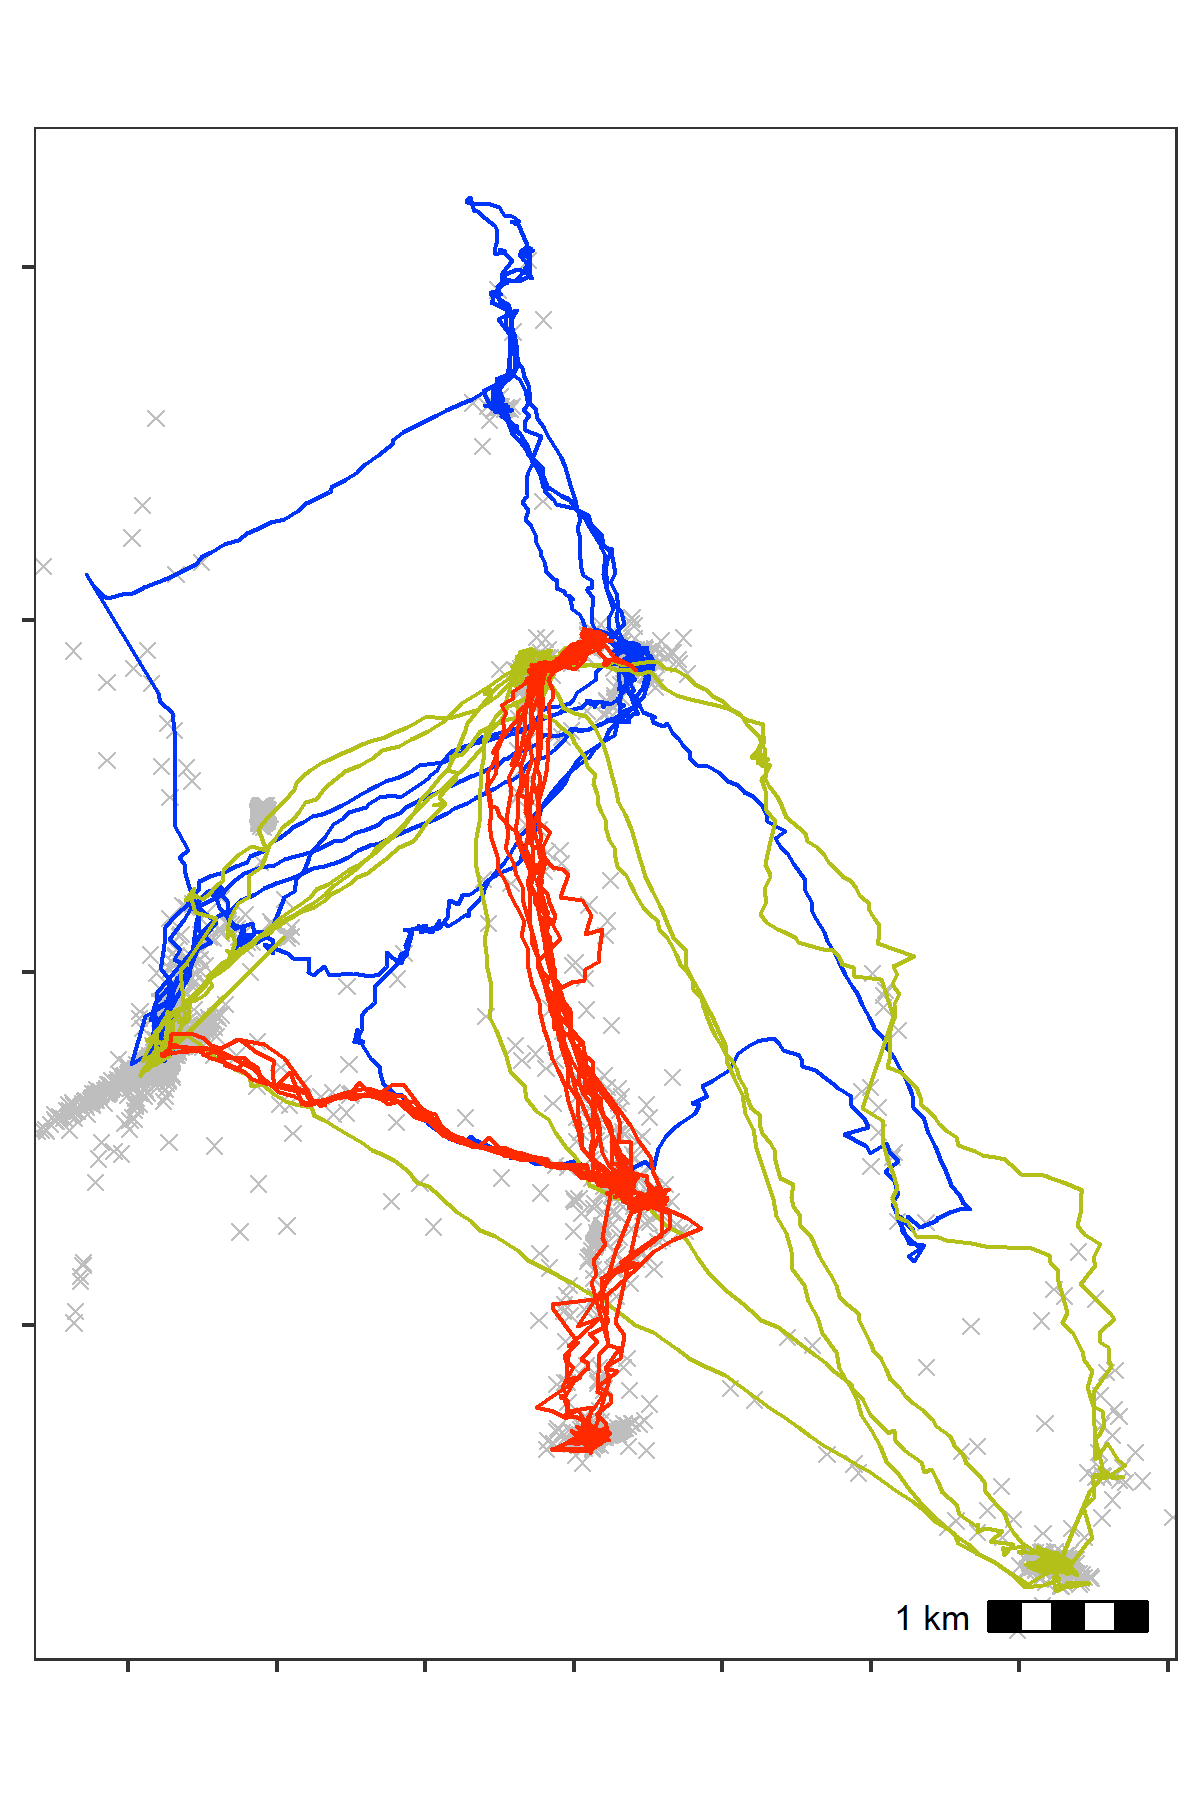
\includegraphics{figures/fig_bat_filter_speed.png}

\hypertarget{median-smoothing}{%
\section{Median smoothing}\label{median-smoothing}}

Apply a 5 point median smooth to the data.

\begin{Shaded}
\begin{Highlighting}[]
\CommentTok{\# since the function modifies in place, we shall make a copy}
\NormalTok{data\_smooth <{-}}\StringTok{ }\KeywordTok{copy}\NormalTok{(data\_split)}

\CommentTok{\# split the data again}
\NormalTok{data\_smooth <{-}}\StringTok{ }\KeywordTok{split}\NormalTok{(data\_smooth, data\_smooth}\OperatorTok{$}\NormalTok{TAG)}
\end{Highlighting}
\end{Shaded}

Remember, \textbf{\texttt{atl\_median\_smooth} MODIFIES IN PLACE}.

\begin{Shaded}
\begin{Highlighting}[]
\CommentTok{\# apply the median smooth to each list element}
\CommentTok{\# no reassignment is required as THE FUNCTION MODIFIES IN PLACE!}
\KeywordTok{invisible}\NormalTok{(}
  \CommentTok{\# the function arguments to atl\_median\_smooth}
  \CommentTok{\# can be passed directly in lapply}
  \KeywordTok{lapply}\NormalTok{(data\_smooth, atl\_median\_smooth,}
         \DataTypeTok{time =} \StringTok{"time"}\NormalTok{, }\DataTypeTok{moving\_window =} \DecValTok{5}\NormalTok{)}
\NormalTok{)}
\end{Highlighting}
\end{Shaded}

\hypertarget{sanity-check-plot-smoothed-data}{%
\subsection{Sanity check: Plot smoothed data}\label{sanity-check-plot-smoothed-data}}

\begin{Shaded}
\begin{Highlighting}[]
\CommentTok{\# recombine split up data that has been smoothed}
\NormalTok{data\_smooth <{-}}\StringTok{ }\KeywordTok{rbindlist}\NormalTok{(data\_smooth)}
\end{Highlighting}
\end{Shaded}

Save the smoothed data plot.

Show the plot.

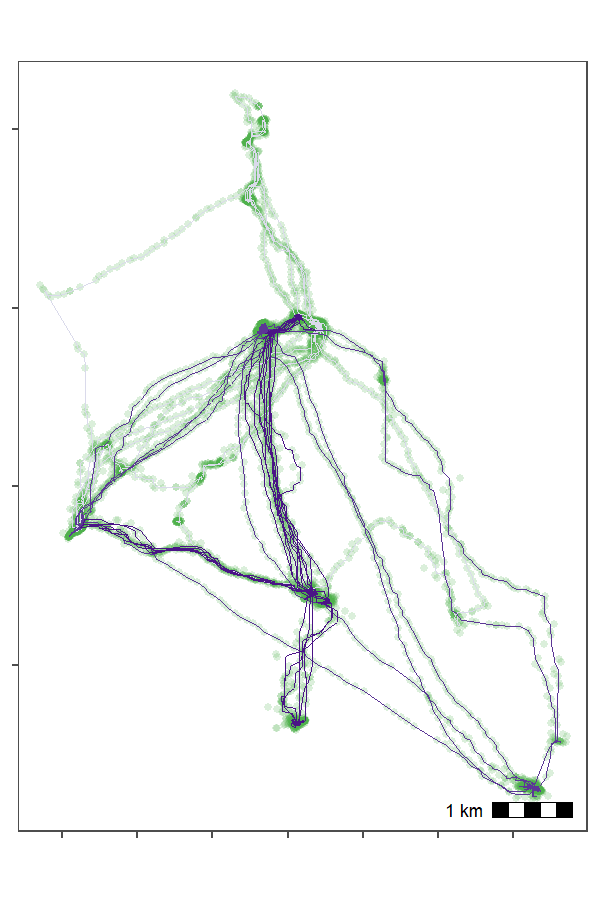
\includegraphics{figures/fig_bat_smooth.png}

\hypertarget{making-residence-patches}{%
\section{Making residence patches}\label{making-residence-patches}}

\hypertarget{calculating-residence-time}{%
\subsection{Calculating residence time}\label{calculating-residence-time}}

First, the data is put through the \texttt{recurse} package to get residence time.

\begin{Shaded}
\begin{Highlighting}[]
\CommentTok{\# load recurse}
\KeywordTok{library}\NormalTok{(recurse)}

\CommentTok{\# split the data}
\NormalTok{data\_smooth <{-}}\StringTok{ }\KeywordTok{split}\NormalTok{(data\_smooth, data\_smooth}\OperatorTok{$}\NormalTok{TAG)}
\end{Highlighting}
\end{Shaded}

Get residence time. Since bats may revisit the same features, we want to prevent confusion between frequent revisits and prolonged residence.

For this, we stop summing residence times within Z metres of a location if the animal exited the area for one hour or more.

\begin{Shaded}
\begin{Highlighting}[]
\CommentTok{\# get residence times}

\NormalTok{data\_residence <{-}}\StringTok{ }\KeywordTok{lapply}\NormalTok{(data\_smooth, }\ControlFlowTok{function}\NormalTok{(dt) \{}
  \CommentTok{\# do basic recurse}
\NormalTok{  dt\_recurse <{-}}\StringTok{ }\KeywordTok{getRecursions}\NormalTok{(}
    \DataTypeTok{x =}\NormalTok{ dt[, }\KeywordTok{c}\NormalTok{(}\StringTok{"X"}\NormalTok{, }\StringTok{"Y"}\NormalTok{, }\StringTok{"time"}\NormalTok{, }\StringTok{"TAG"}\NormalTok{)],}
    \DataTypeTok{radius =} \DecValTok{50}\NormalTok{,}
    \DataTypeTok{timeunits =} \StringTok{"mins"}
\NormalTok{  )}
  
  \CommentTok{\# get revisit stats}
\NormalTok{  dt\_recurse <{-}}\StringTok{ }\KeywordTok{setDT}\NormalTok{(}
\NormalTok{    dt\_recurse[[}\StringTok{"revisitStats"}\NormalTok{]]}
\NormalTok{  )}
  
  \CommentTok{\# count long absences from the area}
\NormalTok{  dt\_recurse[, timeSinceLastVisit }\OperatorTok{:}\ErrorTok{=}
\StringTok{          }\KeywordTok{ifelse}\NormalTok{(}\KeywordTok{is.na}\NormalTok{(timeSinceLastVisit), }\OperatorTok{{-}}\OtherTok{Inf}\NormalTok{, timeSinceLastVisit)]}
\NormalTok{  dt\_recurse[, longAbsenceCounter }\OperatorTok{:}\ErrorTok{=}\StringTok{ }\KeywordTok{cumsum}\NormalTok{(timeSinceLastVisit }\OperatorTok{>}\StringTok{ }\DecValTok{60}\NormalTok{),}
\NormalTok{             by =}\StringTok{ }\NormalTok{.(coordIdx)}
\NormalTok{             ]}
  \CommentTok{\# get data before the first long absence of 60 mins}
\NormalTok{  dt\_recurse <{-}}\StringTok{ }\NormalTok{dt\_recurse[longAbsenceCounter }\OperatorTok{<}\StringTok{ }\DecValTok{1}\NormalTok{, ]}
  
\NormalTok{  dt\_recurse <{-}}\StringTok{ }\NormalTok{dt\_recurse[, }\KeywordTok{list}\NormalTok{(}
    \DataTypeTok{resTime =} \KeywordTok{sum}\NormalTok{(timeInside),}
    \DataTypeTok{fpt =} \KeywordTok{first}\NormalTok{(timeInside),}
    \DataTypeTok{revisits =} \KeywordTok{max}\NormalTok{(visitIdx)}
\NormalTok{  ),}
\NormalTok{  by =}\StringTok{ }\NormalTok{.(coordIdx, x, y)}
\NormalTok{  ]}
  
  \CommentTok{\# prepare and merge existing data with recursion data}
\NormalTok{  dt[, coordIdx }\OperatorTok{:}\ErrorTok{=}\StringTok{ }\KeywordTok{seq}\NormalTok{(}\KeywordTok{nrow}\NormalTok{(dt))]}
  
\NormalTok{  dt <{-}}\StringTok{ }\KeywordTok{merge}\NormalTok{(dt, }
\NormalTok{              dt\_recurse[, }\KeywordTok{c}\NormalTok{(}\StringTok{"coordIdx"}\NormalTok{, }\StringTok{"resTime"}\NormalTok{)], }
              \DataTypeTok{by =} \KeywordTok{c}\NormalTok{(}\StringTok{"coordIdx"}\NormalTok{))}
  
  \KeywordTok{setorderv}\NormalTok{(dt, }\StringTok{"time"}\NormalTok{)}
\NormalTok{\})}
\end{Highlighting}
\end{Shaded}

\hypertarget{sanity-check-residence-time-time-series}{%
\subsection{Sanity check: Residence-time time-series}\label{sanity-check-residence-time-time-series}}

\begin{Shaded}
\begin{Highlighting}[]
\CommentTok{\# bind the list}
\NormalTok{data\_residence <{-}}\StringTok{ }\KeywordTok{rbindlist}\NormalTok{(data\_residence)}

\CommentTok{\# get time as human readable}
\NormalTok{data\_residence[, ts }\OperatorTok{:}\ErrorTok{=}\StringTok{ }\KeywordTok{as.POSIXct}\NormalTok{(time, }\DataTypeTok{origin =} \StringTok{"1970{-}01{-}01"}\NormalTok{)]}
\end{Highlighting}
\end{Shaded}

Save the speed filtered data plot.

Show the plot.

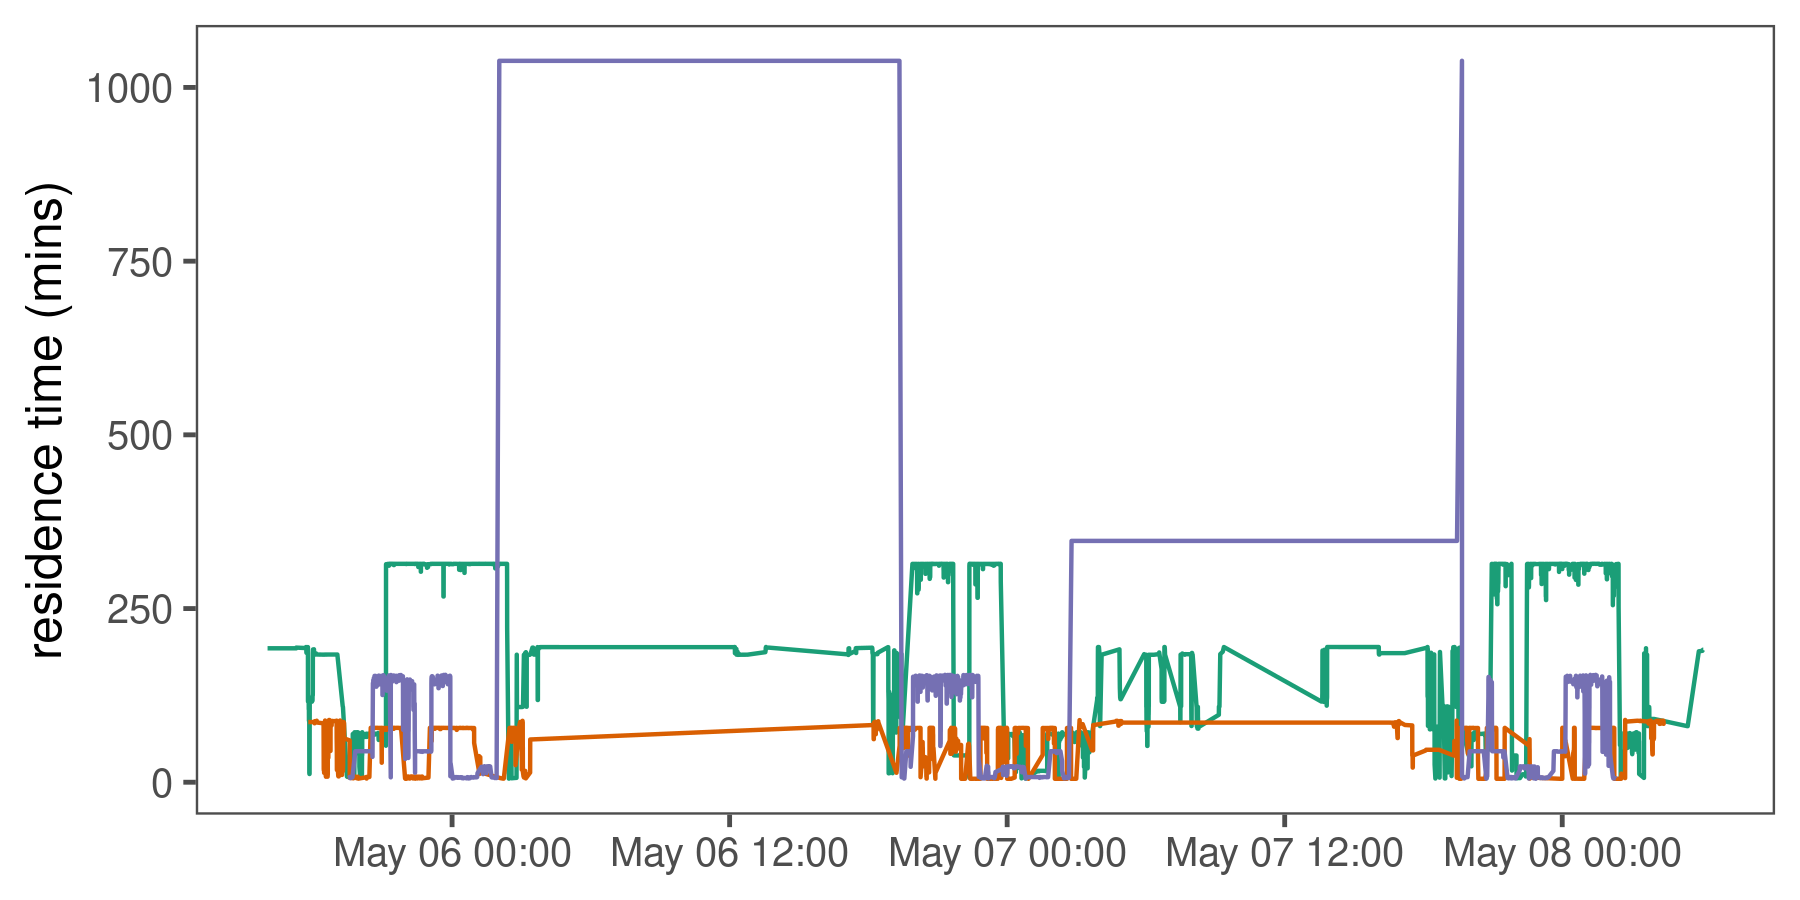
\includegraphics{figures/fig_bat_res_timeseries.png}

\hypertarget{constructing-residence-patches}{%
\subsection{Constructing residence patches}\label{constructing-residence-patches}}

Split the data and construct residence patches.

Some preparation is required. First, the function requires columns \texttt{x}, \texttt{y},
\texttt{time}, and \texttt{id}.

\begin{Shaded}
\begin{Highlighting}[]
\CommentTok{\# add an id column}
\NormalTok{data\_residence[, }\StringTok{\textasciigrave{}}\DataTypeTok{:=}\StringTok{\textasciigrave{}}\NormalTok{(}\DataTypeTok{id =}\NormalTok{ TAG,}
                      \DataTypeTok{x =}\NormalTok{ X, }\DataTypeTok{y =}\NormalTok{ Y)]}

\CommentTok{\# filter for residence time > 5 minutes}
\NormalTok{data\_residence <{-}}\StringTok{ }\NormalTok{data\_residence[resTime }\OperatorTok{>}\StringTok{ }\DecValTok{5}\NormalTok{, ]}

\CommentTok{\# split the data}
\NormalTok{data\_residence <{-}}\StringTok{ }\KeywordTok{split}\NormalTok{(data\_residence, data\_residence}\OperatorTok{$}\NormalTok{TAG)}
\end{Highlighting}
\end{Shaded}

Now segment-cluster into residence patches.

\begin{Shaded}
\begin{Highlighting}[]
\CommentTok{\# segment into residence patches}
\NormalTok{data\_patches <{-}}\StringTok{ }\KeywordTok{lapply}\NormalTok{(data\_residence, atl\_res\_patch,}
                       \DataTypeTok{buffer\_radius =} \DecValTok{25}\NormalTok{)}
\end{Highlighting}
\end{Shaded}

\hypertarget{getting-residence-patch-data}{%
\subsection{Getting residence patch data}\label{getting-residence-patch-data}}

We get the residence patch data as spatial \texttt{sf-MULTIPOLYGON} objects.

\begin{Shaded}
\begin{Highlighting}[]
\CommentTok{\# get data spatials}
\NormalTok{data\_spatials <{-}}\StringTok{ }\KeywordTok{lapply}\NormalTok{(data\_patches, atl\_patch\_summary,}
                        \DataTypeTok{which\_data =} \StringTok{"spatial"}\NormalTok{,}
                        \DataTypeTok{buffer\_radius =} \DecValTok{25}\NormalTok{)}

\CommentTok{\# bind list}
\NormalTok{data\_spatials <{-}}\StringTok{ }\KeywordTok{rbindlist}\NormalTok{(data\_spatials)}

\CommentTok{\# convert to sf}
\KeywordTok{library}\NormalTok{(sf)}
\NormalTok{data\_spatials <{-}}\StringTok{ }\KeywordTok{st\_sf}\NormalTok{(data\_spatials, }\DataTypeTok{sf\_column\_name =} \StringTok{"polygons"}\NormalTok{)}

\CommentTok{\# assign a crs}
\KeywordTok{st\_crs}\NormalTok{(data\_spatials) <{-}}\StringTok{ }\KeywordTok{st\_crs}\NormalTok{(}\DecValTok{2039}\NormalTok{)}
\end{Highlighting}
\end{Shaded}

\hypertarget{write-patch-spatial-representations}{%
\subsection{Write patch spatial representations}\label{write-patch-spatial-representations}}

\begin{Shaded}
\begin{Highlighting}[]
\KeywordTok{st\_write}\NormalTok{(data\_spatials,}
         \DataTypeTok{dsn =} \StringTok{"data/data\_bat\_residence\_patches.gpkg"}\NormalTok{)}
\end{Highlighting}
\end{Shaded}

Write cleaned bat data.

\begin{Shaded}
\begin{Highlighting}[]
\NormalTok{data\_clean <{-}}\StringTok{ }\KeywordTok{fwrite}\NormalTok{(}\KeywordTok{rbindlist}\NormalTok{(data\_smooth),}
                     \DataTypeTok{file =} \StringTok{"data/data\_bat\_smooth.csv"}\NormalTok{)}
\end{Highlighting}
\end{Shaded}

Write patch summary.

\begin{Shaded}
\begin{Highlighting}[]
\CommentTok{\# get summary}
\NormalTok{patch\_summary <{-}}\StringTok{ }\KeywordTok{lapply}\NormalTok{(data\_patches, atl\_patch\_summary)}

\CommentTok{\# bind summary}
\NormalTok{patch\_summary <{-}}\StringTok{ }\KeywordTok{rbindlist}\NormalTok{(patch\_summary)}

\CommentTok{\# write}
\KeywordTok{fwrite}\NormalTok{(patch\_summary,}
       \StringTok{"data/data\_bat\_patch\_summary.csv"}\NormalTok{)}
\end{Highlighting}
\end{Shaded}

\hypertarget{processed-bat-patches}{%
\section{Processed bat patches}\label{processed-bat-patches}}

This figure made in QGIS.

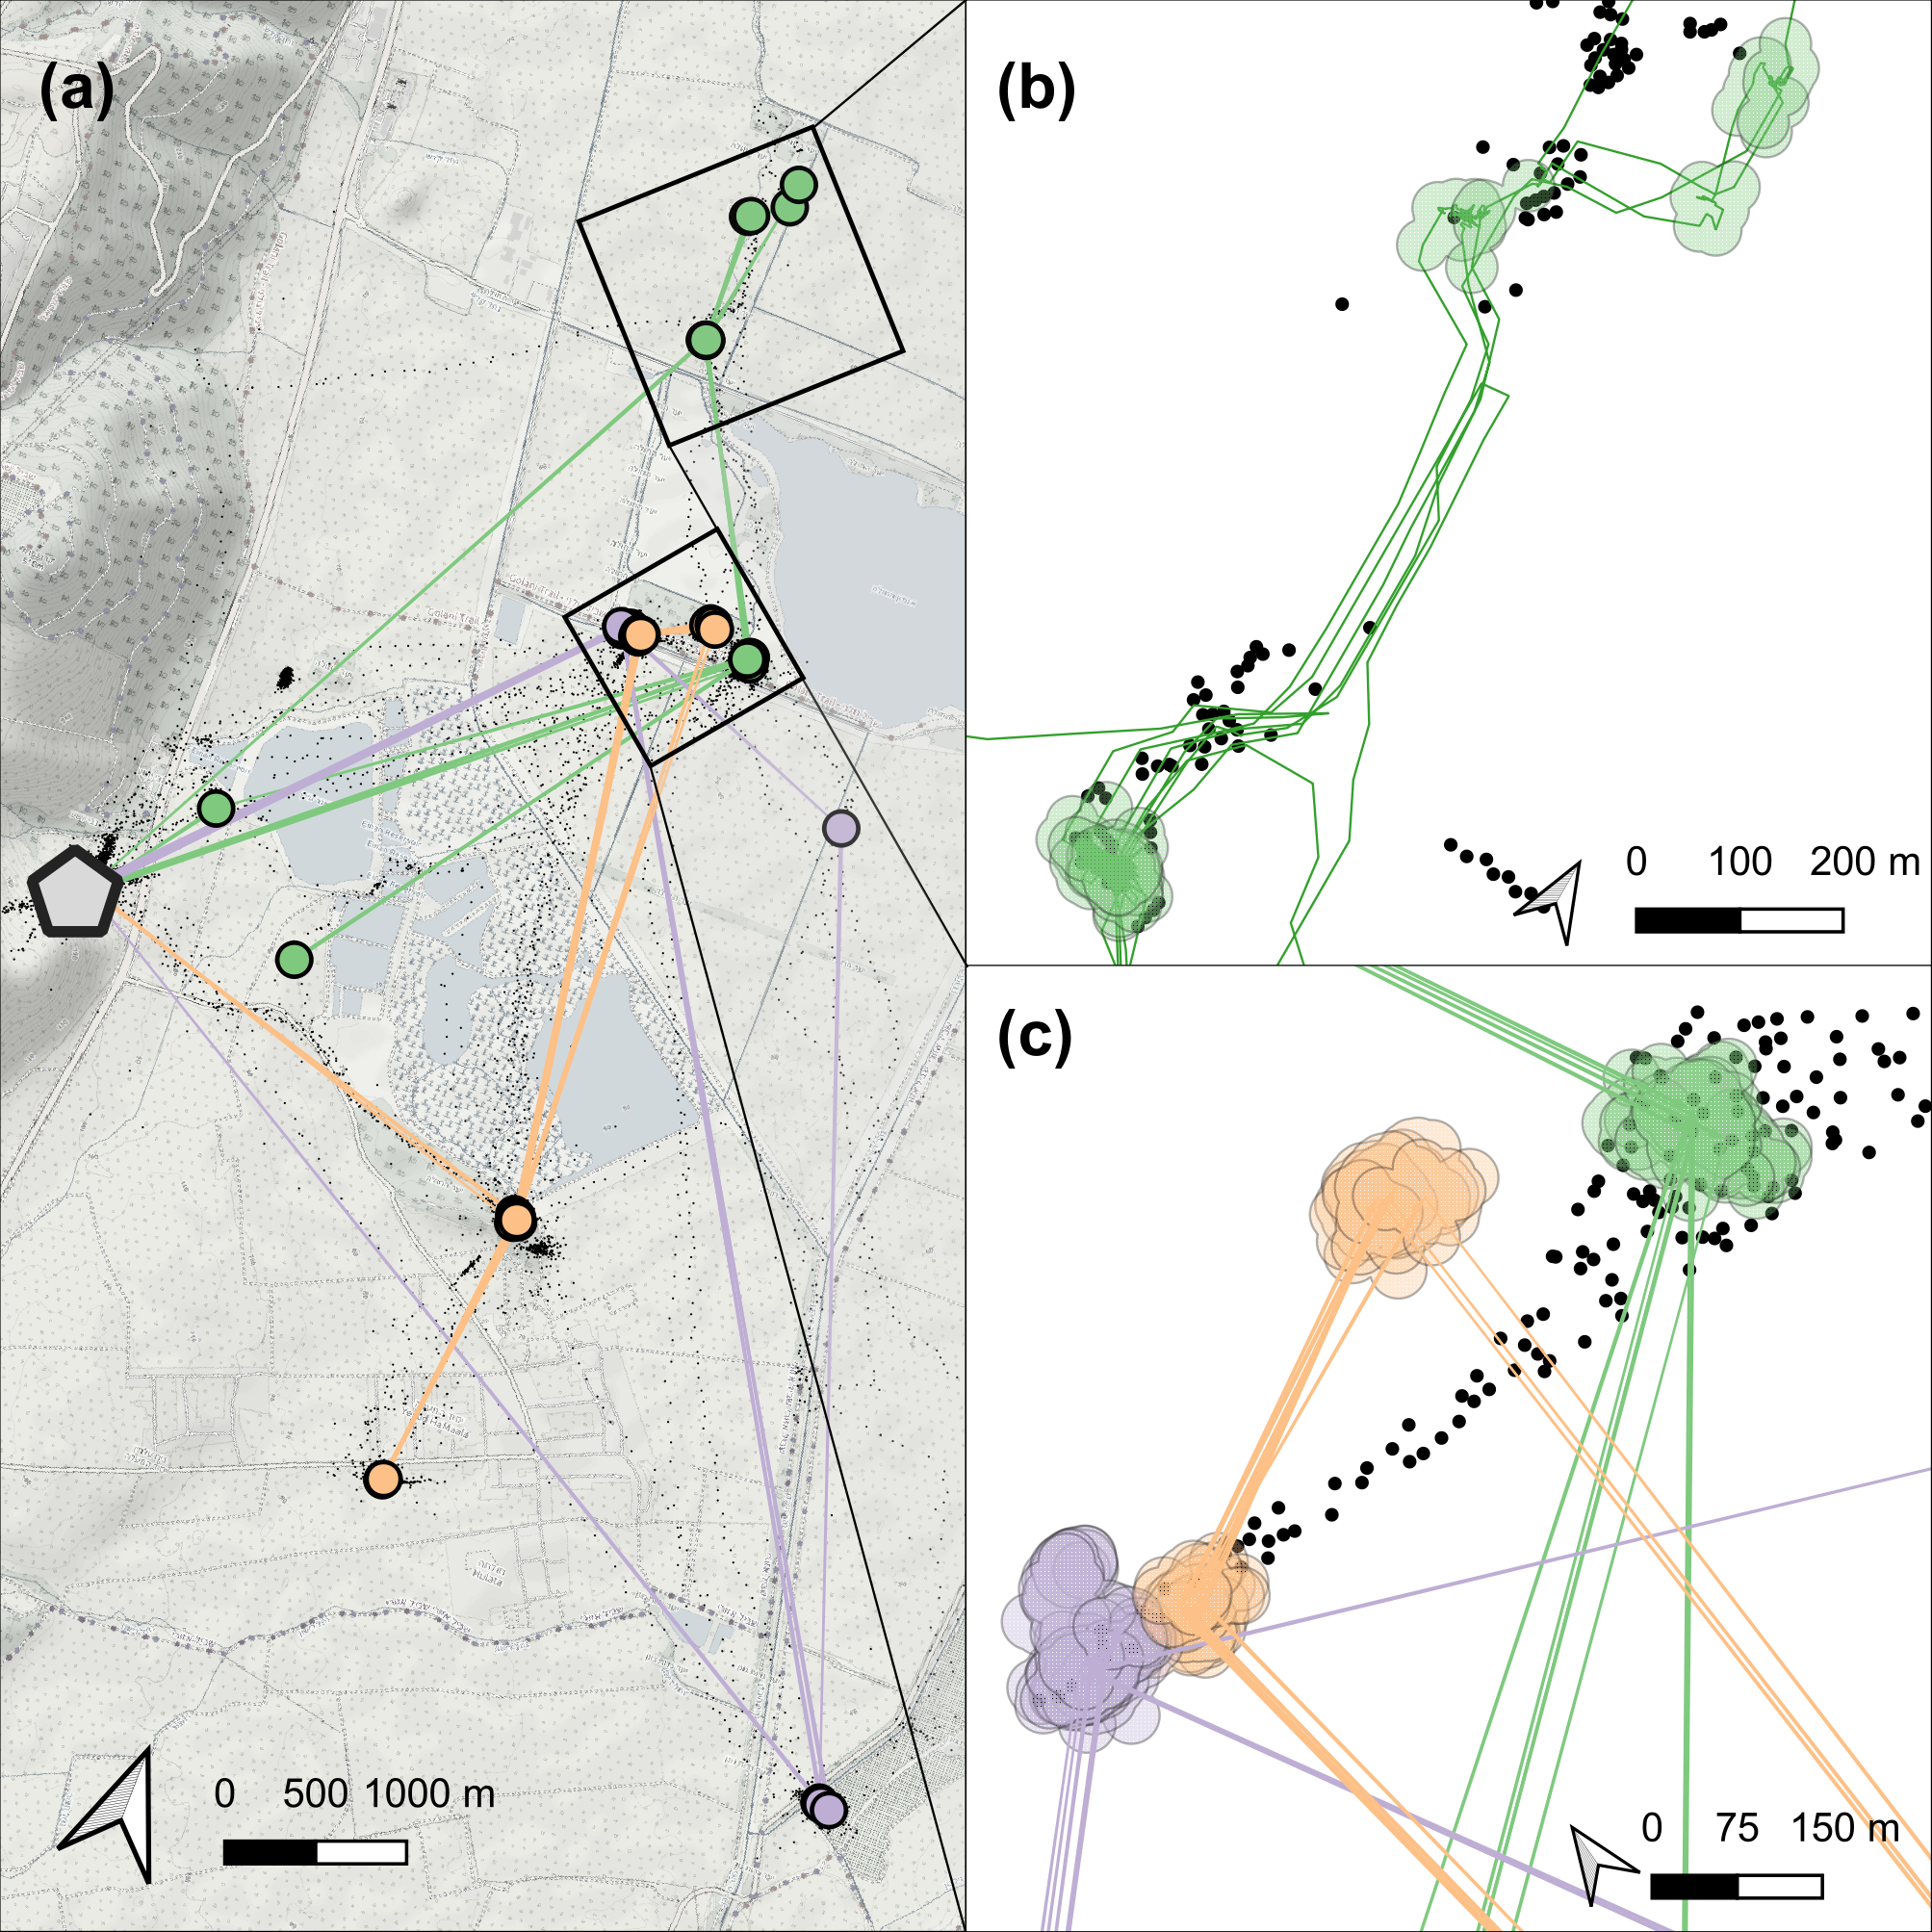
\includegraphics{figures/fig_bat_patches.png}

\hypertarget{references}{%
\chapter{References}\label{references}}

\hypertarget{refs}{}
\begin{cslreferences}
\leavevmode\hypertarget{ref-bjorneraas2010}{}%
Bjørneraas, Kari, Bram Van Moorter, Christer Moe Rolandsen, and Ivar Herfindal. 2010. ``Screening Global Positioning System Location Data for Errors Using Animal Movement Characteristics.'' \emph{The Journal of Wildlife Management} 74 (6): 1361--6. \url{https://doi.org/10.1111/j.1937-2817.2010.tb01258.x}.

\leavevmode\hypertarget{ref-gurarie2017}{}%
Gurarie, Eliezer, Christen H. Fleming, William F. Fagan, Kristin L. Laidre, Jesús Hernández-Pliego, and Otso Ovaskainen. 2017. ``Correlated Velocity Models as a Fundamental Unit of Animal Movement: Synthesis and Applications.'' \emph{Movement Ecology} 5 (1): 13. \url{https://doi.org/10.1186/s40462-017-0103-3}.

\leavevmode\hypertarget{ref-noonan2019}{}%
Noonan, Michael J., Christen H. Fleming, Thomas S. Akre, Jonathan Drescher-Lehman, Eliezer Gurarie, Autumn-Lynn Harrison, Roland Kays, and Justin M. Calabrese. 2019. ``Scale-Insensitive Estimation of Speed and Distance Traveled from Animal Tracking Data.'' \emph{Movement Ecology} 7 (1): 35. \url{https://doi.org/10.1186/s40462-019-0177-1}.
\end{cslreferences}

\end{document}
